% Template for PLoS
%DIF LATEXDIFF DIFFERENCE FILE
%DIF DEL Journal-manuscriptV0.tex   Thu Nov  9 20:02:10 2023
%DIF ADD Journal-manuscript.tex     Thu Nov  9 19:45:08 2023
% Version 3.5 March 2018
%
% % % % % % % % % % % % % % % % % % % % % %
%
% -- IMPORTANT NOTE
%
% This template contains comments intended
% to minimize problems and delays during our production
% process. Please follow the template instructions
% whenever possible.
%
% % % % % % % % % % % % % % % % % % % % % % %
%
% Once your paper is accepted for publication,
% PLEASE REMOVE ALL TRACKED CHANGES in this file
% and leave only the final text of your manuscript.
% PLOS recommends the use of latexdiff to track changes during review, as this will help to maintain a clean tex file.
% Visit https://www.ctan.org/pkg/latexdiff?lang=en for info or contact us at latex@plos.org.
%
%
% There are no restrictions on package use within the LaTeX files except that
% no packages listed in the template may be deleted.
%
% Please do not include colors or graphics in the text.
%
% The manuscript LaTeX source should be contained within a single file (do not use \input, \externaldocument, or similar commands).
%
% % % % % % % % % % % % % % % % % % % % % % %
%
% -- FIGURES AND TABLES
%
% Please include tables/figure captions directly after the paragraph where they are first cited in the text.
%
% DO NOT INCLUDE GRAPHICS IN YOUR MANUSCRIPT
% - Figures should be uploaded separately from your manuscript file.
% - Figures generated using LaTeX should be extracted and removed from the PDF before submission.
% - Figures containing multiple panels/subfigures must be combined into one image file before submission.
% For figure citations, please use "Fig" instead of "Figure".
% See http://journals.plos.org/plosone/s/figures for PLOS figure guidelines.
%
% Tables should be cell-based and may not contain:
% - spacing/line breaks within cells to alter layout or alignment
% - do not nest tabular environments (no tabular environments within tabular environments)
% - no graphics or colored text (cell background color/shading OK)
% See http://journals.plos.org/plosone/s/tables for table guidelines.
%
% For tables that exceed the width of the text column, use the adjustwidth environment as illustrated in the example table in text below.
%
% % % % % % % % % % % % % % % % % % % % % % % %
%
% -- EQUATIONS, MATH SYMBOLS, SUBSCRIPTS, AND SUPERSCRIPTS
%
% IMPORTANT
% Below are a few tips to help format your equations and other special characters according to our specifications. For more tips to help reduce the possibility of formatting errors during conversion, please see our LaTeX guidelines at http://journals.plos.org/plosone/s/latex
%
% For inline equations, please be sure to include all portions of an equation in the math environment.
%
% Do not include text that is not math in the math environment.
%
% Please add line breaks to long display equations when possible in order to fit size of the column.
%
% For inline equations, please do not include punctuation (commas, etc) within the math environment unless this is part of the equation.
%
% When adding superscript or subscripts outside of brackets/braces, please group using {}.
%
% Do not use \cal for caligraphic font.  Instead, use \mathcal{}
%
% % % % % % % % % % % % % % % % % % % % % % % %
%
% Please contact latex@plos.org with any questions.
%
% % % % % % % % % % % % % % % % % % % % % % % %

\documentclass[10pt,letterpaper]{article}
\usepackage[top=0.85in,left=2.75in,footskip=0.75in]{geometry}

% amsmath and amssymb packages, useful for mathematical formulas and symbols
\usepackage{amsmath,amssymb}

% Use adjustwidth environment to exceed column width (see example table in text)
\usepackage{changepage}

%DIF 84a84-85
% Use Unicode characters when possible %DIF > 
\usepackage[utf8x]{inputenc} %DIF > 
%DIF -------

% textcomp package and marvosym package for additional characters
\usepackage{textcomp,marvosym}

% cite package, to clean up citations in the main text. Do not remove.
% \usepackage{cite}

% Use nameref to cite supporting information files (see Supporting Information section for more info)
\usepackage{nameref,hyperref}

% line numbers
\usepackage[right]{lineno}

% ligatures disabled
\usepackage{microtype}
\DisableLigatures[f]{encoding = *, family = * }

% color can be used to apply background shading to table cells only
\usepackage[table]{xcolor}

% array package and thick rules for tables
\usepackage{array}

% create "+" rule type for thick vertical lines
\newcolumntype{+}{!{\vrule width 2pt}}

% create \thickcline for thick horizontal lines of variable length
\newlength\savedwidth
\newcommand\thickcline[1]{%
  \noalign{\global\savedwidth\arrayrulewidth\global\arrayrulewidth 2pt}%
  \cline{#1}%
  \noalign{\vskip\arrayrulewidth}%
  \noalign{\global\arrayrulewidth\savedwidth}%
}

% \thickhline command for thick horizontal lines that span the table
\newcommand\thickhline{\noalign{\global\savedwidth\arrayrulewidth\global\arrayrulewidth 2pt}%
\hline
\noalign{\global\arrayrulewidth\savedwidth}}


% Remove comment for double spacing
%\usepackage{setspace}
%\doublespacing

% Text layout
\raggedright
\setlength{\parindent}{0.5cm}
\textwidth 5.25in
\textheight 8.75in

% Bold the 'Figure #' in the caption and separate it from the title/caption with a period
% Captions will be left justified
\usepackage[aboveskip=1pt,labelfont=bf,labelsep=period,justification=raggedright,singlelinecheck=off]{caption}
\renewcommand{\figurename}{Fig}

% Use the PLoS provided BiBTeX style
% \bibliographystyle{plos2015}

% Remove brackets from numbering in List of References
\makeatletter
\renewcommand{\@biblabel}[1]{\quad#1.}
\makeatother



% Header and Footer with logo
\usepackage{lastpage,fancyhdr,graphicx}
\usepackage{epstopdf}
%\pagestyle{myheadings}
\pagestyle{fancy}
\fancyhf{}
%\setlength{\headheight}{27.023pt}
%\lhead{
\includegraphics[width=2.0in]{PLOS-submission.eps}}
\rfoot{\thepage/\pageref{LastPage}}
\renewcommand{\headrulewidth}{0pt}
\renewcommand{\footrule}{\hrule height 2pt \vspace{2mm}}
\fancyheadoffset[L]{2.25in}
\fancyfootoffset[L]{2.25in}
\lfoot{\today}

%% Include all macros below

\newcommand{\lorem}{{\bf LOREM}}
\newcommand{\ipsum}{{\bf IPSUM}}


% tightlist command for lists without linebreak
\providecommand{\tightlist}{%
  \setlength{\itemsep}{0pt}\setlength{\parskip}{0pt}}


% Pandoc citation processing
\newlength{\cslhangindent}
\setlength{\cslhangindent}{1.5em}
\newlength{\csllabelwidth}
\setlength{\csllabelwidth}{3em}
\newlength{\cslentryspacingunit} % times entry-spacing
\setlength{\cslentryspacingunit}{\parskip}
% for Pandoc 2.8 to 2.10.1
\newenvironment{cslreferences}%
  {}%
  {\par}
% For Pandoc 2.11+
\newenvironment{CSLReferences}[2] % #1 hanging-ident, #2 entry spacing
 {% don't indent paragraphs
  \setlength{\parindent}{0pt}
  % turn on hanging indent if param 1 is 1
  \ifodd #1
  \let\oldpar\par
  \def\par{\hangindent=\cslhangindent\oldpar}
  \fi
  % set entry spacing
  \setlength{\parskip}{#2\cslentryspacingunit}
 }%
 {}
\usepackage{calc}
\newcommand{\CSLBlock}[1]{#1\hfill\break}
\newcommand{\CSLLeftMargin}[1]{\parbox[t]{\csllabelwidth}{#1}}
\newcommand{\CSLRightInline}[1]{\parbox[t]{\linewidth - \csllabelwidth}{#1}\break}
\newcommand{\CSLIndent}[1]{\hspace{\cslhangindent}#1}

\usepackage{multirow}
\usepackage{multicol}
\usepackage{colortbl}
\usepackage{hhline}
\newlength\Oldarrayrulewidth
\newlength\Oldtabcolsep
\usepackage{longtable}
\usepackage{array}
\usepackage{hyperref}
\usepackage{float}
\usepackage{wrapfig}


\usepackage{forarray}
\usepackage{xstring}
\newcommand{\getIndex}[2]{
  \ForEach{,}{\IfEq{#1}{\thislevelitem}{\number\thislevelcount\ExitForEach}{}}{#2}
}

\setcounter{secnumdepth}{0}

\newcommand{\getAff}[1]{
  \getIndex{#1}{McMaster,Madrid}
}
%DIF PREAMBLE EXTENSION ADDED BY LATEXDIFF
%DIF UNDERLINE PREAMBLE %DIF PREAMBLE
\RequirePackage[normalem]{ulem} %DIF PREAMBLE
\RequirePackage{color}\definecolor{RED}{rgb}{1,0,0}\definecolor{BLUE}{rgb}{0,0,1} %DIF PREAMBLE
\providecommand{\DIFaddtex}[1]{{\protect\color{blue}\uwave{#1}}} %DIF PREAMBLE
\providecommand{\DIFdeltex}[1]{{\protect\color{red}\sout{#1}}}                      %DIF PREAMBLE
%DIF SAFE PREAMBLE %DIF PREAMBLE
\providecommand{\DIFaddbegin}{} %DIF PREAMBLE
\providecommand{\DIFaddend}{} %DIF PREAMBLE
\providecommand{\DIFdelbegin}{} %DIF PREAMBLE
\providecommand{\DIFdelend}{} %DIF PREAMBLE
\providecommand{\DIFmodbegin}{} %DIF PREAMBLE
\providecommand{\DIFmodend}{} %DIF PREAMBLE
%DIF FLOATSAFE PREAMBLE %DIF PREAMBLE
\providecommand{\DIFaddFL}[1]{\DIFadd{#1}} %DIF PREAMBLE
\providecommand{\DIFdelFL}[1]{\DIFdel{#1}} %DIF PREAMBLE
\providecommand{\DIFaddbeginFL}{} %DIF PREAMBLE
\providecommand{\DIFaddendFL}{} %DIF PREAMBLE
\providecommand{\DIFdelbeginFL}{} %DIF PREAMBLE
\providecommand{\DIFdelendFL}{} %DIF PREAMBLE
%DIF HYPERREF PREAMBLE %DIF PREAMBLE
\providecommand{\DIFadd}[1]{\texorpdfstring{\DIFaddtex{#1}}{#1}} %DIF PREAMBLE
\providecommand{\DIFdel}[1]{\texorpdfstring{\DIFdeltex{#1}}{}} %DIF PREAMBLE
\newcommand{\DIFscaledelfig}{0.5}
%DIF HIGHLIGHTGRAPHICS PREAMBLE %DIF PREAMBLE
\RequirePackage{settobox} %DIF PREAMBLE
\RequirePackage{letltxmacro} %DIF PREAMBLE
\newsavebox{\DIFdelgraphicsbox} %DIF PREAMBLE
\newlength{\DIFdelgraphicswidth} %DIF PREAMBLE
\newlength{\DIFdelgraphicsheight} %DIF PREAMBLE
% store original definition of \includegraphics %DIF PREAMBLE
\LetLtxMacro{\DIFOincludegraphics}{\includegraphics} %DIF PREAMBLE
\newcommand{\DIFaddincludegraphics}[2][]{{\color{blue}\fbox{\DIFOincludegraphics[#1]{#2}}}} %DIF PREAMBLE
\newcommand{\DIFdelincludegraphics}[2][]{% %DIF PREAMBLE
\sbox{\DIFdelgraphicsbox}{\DIFOincludegraphics[#1]{#2}}% %DIF PREAMBLE
\settoboxwidth{\DIFdelgraphicswidth}{\DIFdelgraphicsbox} %DIF PREAMBLE
\settoboxtotalheight{\DIFdelgraphicsheight}{\DIFdelgraphicsbox} %DIF PREAMBLE
\scalebox{\DIFscaledelfig}{% %DIF PREAMBLE
\parbox[b]{\DIFdelgraphicswidth}{\usebox{\DIFdelgraphicsbox}\\[-\baselineskip] \rule{\DIFdelgraphicswidth}{0em}}\llap{\resizebox{\DIFdelgraphicswidth}{\DIFdelgraphicsheight}{% %DIF PREAMBLE
\setlength{\unitlength}{\DIFdelgraphicswidth}% %DIF PREAMBLE
\begin{picture}(1,1)% %DIF PREAMBLE
\thicklines\linethickness{2pt} %DIF PREAMBLE
{\color[rgb]{1,0,0}\put(0,0){\framebox(1,1){}}}% %DIF PREAMBLE
{\color[rgb]{1,0,0}\put(0,0){\line( 1,1){1}}}% %DIF PREAMBLE
{\color[rgb]{1,0,0}\put(0,1){\line(1,-1){1}}}% %DIF PREAMBLE
\end{picture}% %DIF PREAMBLE
}\hspace*{3pt}}} %DIF PREAMBLE
} %DIF PREAMBLE
\LetLtxMacro{\DIFOaddbegin}{\DIFaddbegin} %DIF PREAMBLE
\LetLtxMacro{\DIFOaddend}{\DIFaddend} %DIF PREAMBLE
\LetLtxMacro{\DIFOdelbegin}{\DIFdelbegin} %DIF PREAMBLE
\LetLtxMacro{\DIFOdelend}{\DIFdelend} %DIF PREAMBLE
\DeclareRobustCommand{\DIFaddbegin}{\DIFOaddbegin \let\includegraphics\DIFaddincludegraphics} %DIF PREAMBLE
\DeclareRobustCommand{\DIFaddend}{\DIFOaddend \let\includegraphics\DIFOincludegraphics} %DIF PREAMBLE
\DeclareRobustCommand{\DIFdelbegin}{\DIFOdelbegin \let\includegraphics\DIFdelincludegraphics} %DIF PREAMBLE
\DeclareRobustCommand{\DIFdelend}{\DIFOaddend \let\includegraphics\DIFOincludegraphics} %DIF PREAMBLE
\LetLtxMacro{\DIFOaddbeginFL}{\DIFaddbeginFL} %DIF PREAMBLE
\LetLtxMacro{\DIFOaddendFL}{\DIFaddendFL} %DIF PREAMBLE
\LetLtxMacro{\DIFOdelbeginFL}{\DIFdelbeginFL} %DIF PREAMBLE
\LetLtxMacro{\DIFOdelendFL}{\DIFdelendFL} %DIF PREAMBLE
\DeclareRobustCommand{\DIFaddbeginFL}{\DIFOaddbeginFL \let\includegraphics\DIFaddincludegraphics} %DIF PREAMBLE
\DeclareRobustCommand{\DIFaddendFL}{\DIFOaddendFL \let\includegraphics\DIFOincludegraphics} %DIF PREAMBLE
\DeclareRobustCommand{\DIFdelbeginFL}{\DIFOdelbeginFL \let\includegraphics\DIFdelincludegraphics} %DIF PREAMBLE
\DeclareRobustCommand{\DIFdelendFL}{\DIFOaddendFL \let\includegraphics\DIFOincludegraphics} %DIF PREAMBLE
%DIF END PREAMBLE EXTENSION ADDED BY LATEXDIFF

\begin{document}
\vspace*{0.2in}


% Title must be 250 characters or less.
\begin{flushleft}
{\Large
\textbf\DIFdelbegin %DIFDELCMD < \newline{Multimodal spatial availability: a singly-constrained
%DIFDELCMD < measure of competitive accessibility considering multiple
%DIFDELCMD < modes} %%%
\DIFdelend \DIFaddbegin \newline{Multimodal spatial availability: a singly-constrained
measure of accessibility considering multiple
modes} \DIFaddend % Please use "sentence case" for title and headings (capitalize only the first word in a title (or heading), the first word in a subtitle (or subheading), and any proper nouns).
}
\newline
% Insert author names, affiliations and corresponding author email (do not include titles, positions, or degrees).
\\
Anastasia Soukhov\textsuperscript{\getAff{McMaster}}\textsuperscript{*},
Javier Tarriño-Ortiz\textsuperscript{\getAff{Madrid}},
Julio A. Soria-Lara\textsuperscript{\getAff{Madrid}},
Antonio Páez\textsuperscript{\getAff{McMaster}}\\
\bigskip
\textbf{\getAff{McMaster}}Department of Earth, Environment and Society,
McMaster University, Hamilton, Canada\\
\textbf{\getAff{Madrid}}Centro de Investigación del Transporte
(TRANSyT), Universidad Politécnica de Madrid, Madrid, Spain\\
\bigskip
* Corresponding author: soukhoa@mcmaster.ca (AS)\\
\end{flushleft}
% Please keep the abstract below 300 words
\section*{Abstract}
\DIFdelbegin \DIFdel{An increasing number of studies within the domain of transportation
planning are concerned with the inequities in accessibility to
opportunities. A dimension of these inequities arises from differences
in access by mode type (e.g.,
commuting using a car as opposed to
transit). However, methods implemented in current accessibility literature are lacking within the
context of
multimodal analysis. This
paper presents an extension of }\DIFdelend \DIFaddbegin \DIFadd{Recent research has aimed to address the way opportunities are counted
in accessibility analysis. In conventional accessibility measures,
opportunities are often multiply counted, which leads to values of
accessibility that are difficult to interpret. Constraining the
calculations to match a known quantity ensures that the measurements sum
up to a predetermined quantity (i.e., the total number of
opportunities), and so each value can be meaningfully related to this
total. A recent effort is }\DIFaddend spatial availability, a singly-constrained
\DIFdelbegin \DIFdel{competitive accessibility measure, for the context of
multimodal accessibility analysis. We first illustrate the features of
spatial availability that lend itself to multimodal analysis. We then
demonstrate its use on the case study of Low Emission Zones in Madrid
(Spain) and highlight how this policy intervention changes the
accessibility of populations using different modes . In summary, spatial
availability can be used to create and interpret multimodal policy
intervention scenarios unlike previous methods: this creation and
interpretation can help regions envision a more sustainable and
equitable access-to-opportunity landscape. }\DIFdelend \DIFaddbegin \DIFadd{accessibility measure. In this paper we extend spatial availability for
use in the case of multiple modes or, more generally, heterogeneous
population segments with distinct travel behaviors. After deriving a
multimodal version of spatial availability, we proceed to illustrate its
features using a synthetic example. Next, we apply it to an empirical
example in Madrid, Spain. We conclude the paper with suggestions for
future research.
}\DIFaddend 

% Please keep the Author Summary between 150 and 200 words
% Use first person. PLOS ONE authors please skip this step.
% Author Summary not valid for PLOS ONE submissions.

\linenumbers

% Use "Eq" instead of "Equation" for equation citations.
\hypertarget{introduction}{%
\section{Introduction}\label{introduction}}

\DIFdelbegin \DIFdel{Implementing urban policies that re-shape cities through accessibility
gains (i.e., the }\emph{\DIFdel{potential to interact}} %DIFAUXCMD
\DIFdel{with opportunities as a result of land-use mix and
transport systems as originally defined by
}\DIFdelend \DIFaddbegin \DIFadd{Accessibility is a key concept in the analysis of land use and
transportation systems }\DIFaddend {[}\DIFaddbegin \DIFadd{e.g., }\DIFaddend 1\DIFaddbegin \DIFadd{,2,3}\DIFaddend {]}\DIFdelbegin \DIFdel{) have been widely applied within the transportation literature
and is increasingly discussed by planners }\DIFdelend \DIFaddbegin \DIFadd{, and too is coming of age from
the perspective of planning }\DIFaddend {[}\DIFdelbegin \DIFdel{2--5}\DIFdelend \DIFaddbegin \DIFadd{see }\emph{\DIFadd{inter alia}}\DIFadd{, 4,5--8}\DIFaddend {]}.
\DIFdelbegin \DIFdel{An important
challenge in the identification of interventions that equitably
transform cities is the effective evaluation of }\emph{\DIFdel{trade-offs}}%DIFAUXCMD
\DIFdel{:
cities are complex and dynamic ecologies, and advantaging one component
of the city can disadvantage another area, population, or sub-component
In this way, policy evaluation should take a }\emph{\DIFdel{systems}} %DIFAUXCMD
\DIFdel{approach
}\DIFdelend \DIFaddbegin \DIFadd{Beginning with the work of Hansen }\DIFaddend {[}\DIFdelbegin \DIFdel{6}\DIFdelend \DIFaddbegin \DIFadd{1}\DIFaddend {]}\DIFdelbegin \DIFdel{. One way of considering systems is from the perspective of the
}\emph{\DIFdel{finite}}%DIFAUXCMD
\DIFdel{. As an illustration, consider the amount of transport
space within a city: the amount is typically finite so re-allocating
road space away from one mode directly impacts the performance of the
others (see the literature on road space reallocation e.g., }\DIFdelend \DIFaddbegin \DIFadd{, accessibility measures have
been widely used to evaluate the efficiency of transportation systems
when combined with the distribution of opportunities in space }\DIFaddend {[}\DIFdelbegin \DIFdel{7}\DIFdelend \DIFaddbegin \DIFadd{9}\DIFaddend {]}\DIFdelbegin \DIFdel{).
Evaluating policy impacts in the context of }\emph{\DIFdel{finity}} %DIFAUXCMD
\DIFdel{provides a way
to contextualize the balance of trade-offs that the citizens of a city
should tolerate.
}\DIFdelend \DIFaddbegin \DIFadd{.
As such, it is a holistic measure of spatial systems that measures the
ease of reaching destinations }{[}\DIFadd{10,11}{]}\DIFadd{.
}\DIFaddend 

\DIFdelbegin \DIFdel{From the perspective of urban transport systems }\DIFdelend \DIFaddbegin \DIFadd{In practice, the most common form of accessibility measure is based on
the gravity model. These measures are sums of weighted opportunities
around a focal point (i.e., a potential origin), based on how expensive
it is to reach them. Recent research in accessibility analysis has paid
attention to the way opportunities are counted in the pertinent
calculations. Conventionally, the sums are not constrained, which means
that the same opportunity can enter the sum for different origins.
Counting the same opportunity multiple times treats it as if it was
inexhaustible. But opportunities in general are not inexhaustible, and
in fact some of them are by definition exclusive: for example, once a
job is taken up by someone in the population, the same job is no longer
available for any other person to take. More generally, opportunities
are subject to congestion: for example, multiple people can obtain
services from the same family doctor, but the more people who do}\DIFaddend , \DIFdelbegin \DIFdel{location-based
accessibility measures have been used in the
context of policy
evaluation. For instance, }\DIFdelend \DIFaddbegin \DIFadd{the
more congested the service will be.
}

\DIFadd{The issue of congestion in accessibility measures was the motivation for
the development of floating catchment area approaches }\DIFaddend {[}\DIFdelbegin \DIFdel{8}\DIFdelend \DIFaddbegin \DIFadd{12,13}\DIFaddend {]}\DIFdelbegin \DIFdel{assesses the transit accessibility gains to healthcare and employment opportunities for disadvantaged
neighbourhood in Columbus, Ohio, USA after the transit system's
re-design and
introduction of a rapid bus system. However, a limitation
of this study, like others that implement accessibility measures, is
they donot calculate results under a }\emph{\DIFdel{constrained}} %DIFAUXCMD
\DIFdel{framework i.e., one of }\emph{\DIFdel{finity}}%DIFAUXCMD
\DIFdel{.
The citizens of Columbus should experience
quantitative accessibility gains - but is it at the expense of access
using other modes? As another example,}\DIFdelend \DIFaddbegin \DIFadd{. While
these approaches purport to account for congestion, Paez et al. }\DIFaddend {[}\DIFdelbegin \DIFdel{9}\DIFdelend \DIFaddbegin \DIFadd{14}\DIFaddend {]}
\DIFdelbegin \DIFdel{implements a modified
cumulative opportunity measure to assess differences between private
vehicle and transit system accessibility to jobs in Melbourne, but a
similar question remains: does the accessibility afforded to
the private
vehicle using population come at the expense of accessibility losses to
transit users?
}%DIFDELCMD < 

%DIFDELCMD < %%%
\DIFdelend \DIFaddbegin \DIFadd{demonstrate that in general they do not solve the issue of multiple
counting of opportunities, thus leading to biases in the calculation of
total demand and supply, sometimes inflating them, other times deflating
them. In response to this, recent research has paid closer attention to
the way opportunities are counted in accessibility analysis. Paez et al.
}\DIFaddend {[}\DIFdelbegin \DIFdel{8}\DIFdelend \DIFaddbegin \DIFadd{14}\DIFaddend {]}\DIFdelbegin \DIFdel{and }\DIFdelend \DIFaddbegin \DIFadd{, for example, tackle floating catchment area methods and
introduce a normalization of the impedance matrix to allocate the
population and then the level of service proportionally. More recently,
Soukhov et al. }\DIFaddend {[}\DIFdelbegin \DIFdel{9}\DIFdelend \DIFaddbegin \DIFadd{15}\DIFaddend {]} \DIFdelbegin \DIFdel{both use }\emph{\DIFdel{non-competitive}} %DIFAUXCMD
\DIFdel{accessibility
measures. There is a branch of
location-based accessibilitymeasures
that do incorporate the effect of competition for opportunities by the
population in the region. However, we argue that these existing methods
fall short in acknowledging the
}\emph{\DIFdel{finity}} %DIFAUXCMD
\DIFdel{of opportunities. For
instance, }\DIFdelend \DIFaddbegin \DIFadd{introduced a singly-constrained measure of
accessibility, called spatial availability, that employs a similar, but
more sophisticated proportional allocation mechanism. The work of these
authors show that floating catchment area methods can be seen as
singly-constrained accessibility measures, and improve on existing
approaches by guaranteeing that each opportunity is counted only once -
in other words, treating opportunities as }\emph{\DIFadd{finite}}\DIFadd{. The
proportional allocation of spatial availability constrains the
calculations to match a known quantity, therefore ensuring that the
measurements sum up to a predetermined quantity (i.e., the total number
of opportunities), and so each value can be meaningfully related to this
total.
}

\DIFadd{A limitation of spatial availability as introduced by Soukhov et al.
}\DIFaddend {[}\DIFdelbegin \DIFdel{10}\DIFdelend \DIFaddbegin \DIFadd{15}\DIFaddend {]} \DIFdelbegin \DIFdel{applies a competitive measure, two-step floating
catchment approach (2SFCA), for }\DIFdelend \DIFaddbegin \DIFadd{is that it was developed for the case of a homogeneous
population, for example for }\DIFaddend the case of \DIFdelbegin \DIFdel{access to healthcare
services in Florida for both a multimodal network and a single modal
network.
While the differences in modal access are discussed, the question of how the advantage in access afforded by one mode over
another impacts access for different mode users is unanswered. }%DIFDELCMD < 

%DIFDELCMD < %%%
\DIFdel{This
question of how much one mode-using population can access at the
expense of another mode-using population is a pertinent equity question
in the evaluation of policy scenarios that are multimodal . For instance, consider the impact of a low emission zone (LEZ). LEZ is a policy of spatial and modal discrimination: the circulation of vehicles that are
excessively polluting are restricted in specific regions. In the
recognition that opportunities are finite, the implementation of a LEZ
explicitly reduces the access that the population using polluting
vehicles has to opportunities. This restriction allows the population
using other more sustainable modes to potentially have a higher level of access than before the LEZ implementation. This evaluation is especially
urgent as LEZ are currently in effect in cities globally; their
reception has been mixed }\DIFdelend \DIFaddbegin \DIFadd{a single mode of transportation.
However, the finite nature of opportunities makes the analysis of
heterogeneous populations very relevant. In the case of multiple modes
of transportation, people who travel by slower modes (e.g., active
modes) can usually reach fewer opportunities than people who travel by
faster modes and whose range is typically far wider (e.g., car). This
implies that slower travelers will often face increased competition for
local opportunities from travelers who can reach said opportunities from
farther afield.
}

\DIFadd{The objective of this paper is to address this limitation of spatial
availability. Our primary motivation is to extend spatial availability
for the case of multimodal accessibility, but it is worthwhile noting
that this is in fact just one case of heterogeneous populations (i.e.,
travel by different modes). The method itself can easily accommodate
other forms of heterogeneity, for example variations in travel behavior
between older and younger adults }\DIFaddend {[}\DIFdelbegin \DIFdel{11}\DIFdelend \DIFaddbegin \DIFadd{e.g., 16}\DIFaddend {]}\DIFdelbegin \DIFdel{and may be having negative impacts on
disadvantaged populations who have become mobility-restricted
}\DIFdelend \DIFaddbegin \DIFadd{, the propensity of older
adults to use different modes of transportation }\DIFaddend {[}\DIFdelbegin \DIFdel{12,
13}\DIFdelend \DIFaddbegin \DIFadd{e.g., 17}\DIFaddend {]}\DIFdelbegin \DIFdel{. Measures that evaluate the accessibility of modes given
both }\emph{\DIFdel{constrained}} %DIFAUXCMD
\DIFdel{and }\emph{\DIFdel{competitive}} %DIFAUXCMD
\DIFdel{considerations are
lacking in the literature, but are needed, to evaluate such policy
interventions impact on accessibility.
}%DIFDELCMD < 

%DIFDELCMD < %%%
\DIFdel{In }\DIFdelend \DIFaddbegin \DIFadd{, the
usually shorter trip lengths of children compared to grown-ups }\DIFaddend {[}\DIFdelbegin \DIFdel{14}\DIFdelend \DIFaddbegin \DIFadd{e.g.,
18}\DIFaddend {]}\DIFdelbegin \DIFdel{, we
introduce spatial availability, a type of location-based
accessibilitymeasure that is both }\emph{\DIFdel{constrained}} %DIFAUXCMD
\DIFdel{and
}\emph{\DIFdel{competitive}}%DIFAUXCMD
\DIFdel{. In this paper, we extend the spatial availability
measure into a multimodal framework and explore its use in answering the
question outlined: }\emph{\DIFdel{``given opportunities are finite, how many are
available to a given location depending on the mode used?''.}} %DIFAUXCMD
\DIFdel{The answer
to this question quantifies how many opportunities can be accessed,
considering competition, for different modes. To foreground this
exploration, in Section 2, we discuss short falls of a few existing
location-based measures in comparison to spatial availability }\DIFdelend \DIFaddbegin \DIFadd{, or the more limited travel ranges of single parents }{[}\DIFadd{e.g.,
19}{]}\DIFadd{.
}

\DIFadd{The paper rest of this paper is organized as follows. In Section 2 we
provide a brief review of multimodal accessibility. In the following
Section 3 we demonstrate the derivation of the new spatial availability
expression for multiple modes. In Section 4 we illustrate relevant
issues }\DIFaddend through a synthetic example. \DIFdelbegin \DIFdel{In Section 3, the spatial availability of }\DIFdelend \DIFaddbegin \DIFadd{This is followed in Section 5 by }\DIFaddend an
empirical example \DIFdelbegin \DIFdel{of the LEZ in the }\DIFdelend \DIFaddbegin \DIFadd{using data from the }\DIFaddend city of Madrid \DIFdelbegin \DIFdel{, Spain is calculated.
We demonstrate how the
restriction of car circulation could have
impacted the spatial availability of opportunities for
each
sub-population using }\DIFdelend \DIFaddbegin \DIFadd{after the
implementation of its Low Emission Zones (LEZ). Data for this example
comes from the city's 2018 travel survey. The example shows the
differences in spatial availability within and outside the LEZ for
travelers using different modes, namely car, }\DIFaddend transit, cycling and
walking\DIFdelbegin \DIFdel{modes}\DIFdelend . In Section \DIFdelbegin \DIFdel{4}\DIFdelend \DIFaddbegin \DIFadd{6}\DIFaddend , we provide concluding remarks on the strengths of
the use of spatial availability as a multimodal accessibility measure\DIFdelbegin \DIFdel{and }\DIFdelend \DIFaddbegin \DIFadd{,
and discuss }\DIFaddend potential future uses in policy planning scenarios \DIFaddbegin \DIFadd{as well
as directions for future research}\DIFaddend .

\DIFdelbegin %DIFDELCMD < \hypertarget{a-review-of-multimodal-accessibility-measures}{%
%DIFDELCMD < \section{A review of multimodal accessibility
%DIFDELCMD < measures}\label{a-review-of-multimodal-accessibility-measures}}
%DIFDELCMD < %%%
\DIFdelend \DIFaddbegin \hypertarget{a-brief-review-of-multimodal-accessibility}{%
\section{A brief review of multimodal
accessibility}\label{a-brief-review-of-multimodal-accessibility}}
\DIFaddend 

Location-based accessibility indicators are quantitative measures of
\emph{potential} interaction with opportunities for locations within a
given region: they are \DIFdelbegin \DIFdel{a product }\DIFdelend \DIFaddbegin \DIFadd{summary measures }\DIFaddend of the relationship between
land-use and transport systems. Arguably\DIFaddbegin \DIFadd{, }\DIFaddend the most commonly used \DIFdelbegin \DIFdel{location-based
measured are
}\DIFdelend \DIFaddbegin \DIFadd{are
measures based on the gravity model }{[}\DIFadd{20}{]}\DIFadd{, of which }\DIFaddend cumulative
opportunity measures and weighted cumulative opportunity measures \DIFaddbegin \DIFadd{are
particular forms }\DIFaddend {[}\DIFdelbegin \DIFdel{2}\DIFdelend \DIFaddbegin \DIFadd{5}\DIFaddend {]}. These measures \DIFdelbegin \DIFdel{weight the opportunities that can be potentially interacted with from origin
}\DIFdelend \DIFaddbegin \DIFadd{assign a weight to
opportunities based on how easy it is to reach them. Given an origin
(}\DIFaddend \(i\)\DIFdelbegin \DIFdel{to destination }\DIFdelend \DIFaddbegin \DIFadd{) and a destination (}\DIFaddend \(j\)\DIFdelbegin \DIFdel{based on some sort of travel cost function }\DIFdelend \DIFaddbegin \DIFadd{), an impedance function
\(f^{m}(c^m_{ij})\) converts the cost of travel }\DIFaddend (e.g., \DIFdelbegin \DIFdel{travel time, fare,
travel distance) otherwise known as a travel impedance function
\(f^{m}(c^m_{ij})\). Many weighted cumulative opportunities (often
referred to as the gravity-based measure) originate from the measure
proposed by }\DIFdelend \DIFaddbegin \DIFadd{time, money,
generalized cost) into a score that represents the propensity for
interaction. These measures originate from that proposed by Hansen
}\DIFaddend {[}1{]}, which can take the following \DIFdelbegin \DIFdel{multimodal form }\DIFdelend \DIFaddbegin \DIFadd{form in the multimodal case}\DIFaddend :
\(S_i^m = \sum_j O_j f^m(c_{ij}^m)\) where \(m\) is a set of modes which
have mode-specific travel costs \DIFdelbegin \DIFdel{\((c_{ij}^m)\) and}\DIFdelend \DIFaddbegin \DIFadd{(\(c_{ij}^m\)) and/or }\DIFaddend travel impedance
functions \DIFaddbegin \DIFadd{(}\DIFaddend \(f^m(\cdot)\)\DIFaddbegin \DIFadd{)}\DIFaddend .

\DIFdelbegin \DIFdel{The }\DIFdelend Hansen-type \DIFdelbegin \DIFdel{measure does not consider competition between modes nor
is it constrained. As }\DIFdelend \DIFaddbegin \DIFadd{accessibility is not constrained, which is to say it does
not consider the opportunities as finite. To cite }\DIFaddend an example, \DIFdelbegin \DIFdel{the work of }\DIFdelend \DIFaddbegin \DIFadd{Tahmasbi
et al. }\DIFaddend {[}\DIFdelbegin \DIFdel{15}\DIFdelend \DIFaddbegin \DIFadd{21}\DIFaddend {]} \DIFdelbegin \DIFdel{uses the
}\DIFdelend \DIFaddbegin \DIFadd{use }\DIFaddend Hansen-type \DIFdelbegin \DIFdel{measure to measure }\DIFdelend \DIFaddbegin \DIFadd{accessibility to assess }\DIFaddend the potential
interaction with retail locations \DIFdelbegin \DIFdel{using }\DIFdelend \DIFaddbegin \DIFadd{by three modes: }\DIFaddend walking, public
transit, and car \DIFdelbegin \DIFdel{modes \(m\)}\DIFdelend \DIFaddbegin \DIFadd{(i.e., \(m = w, p, c\))}\DIFaddend . \(S_i^m\) is the sum of retail
locations \(j\) that can potentially be \DIFdelbegin \DIFdel{interacted
with }\DIFdelend \DIFaddbegin \DIFadd{reached }\DIFaddend under the travel
impedance as calculated for each \(i\) and \(m\). In other words, \DIFdelbegin \DIFdel{each }\DIFdelend \DIFaddbegin \DIFadd{for
each origin }\DIFaddend \(i\) \DIFdelbegin \DIFdel{has three \(S_i\) values, one per \(m\)}\DIFdelend \DIFaddbegin \DIFadd{three accessibility scores are calculated}\DIFaddend . In this
work, \DIFdelbegin \DIFdel{they demonstrate that the car mode has the highest
\(S_i^{m=car}\) }\DIFdelend \DIFaddbegin \DIFadd{Tahmasbi et al. }{[}\DIFadd{21}{]} \DIFadd{show that car travel affords the highest
\(S_i^{m}\) }\DIFaddend values in the majority of \(i\), i.e., \DIFdelbegin \DIFdel{populations using
}\DIFdelend \DIFaddbegin \DIFadd{travelers who use }\DIFaddend a
car can potentially \DIFdelbegin \DIFdel{interact with the most }\DIFdelend \DIFaddbegin \DIFadd{reach more }\DIFaddend retail opportunities than populations
using other modes. However, \DIFdelbegin \DIFdel{the higher \(S_i^{m=car}\)
values are not
a result of lower }\DIFdelend \DIFaddbegin \DIFadd{higher \(S_i^{m}\) values for car do not
affect the values of }\DIFaddend \(S_i^{m}\) \DIFdelbegin \DIFdel{values }\DIFdelend for other modes: \DIFdelbegin \DIFdel{it
is not assumed that car-using populations potentially accessing more
opportunitiestake away potential opportunities for other populations
within the measure (no consideration for competition). This measure is also not constrained: there is
no global maximum for \(S_i\) or
\(S_i^m\) values,they are presented as a population normalized
accessibilityindex. This makes the }\DIFdelend \DIFaddbegin \DIFadd{in effect, each mode
is analyzed as if the others did not exist. Since the measure is not
constrained, each opportunity is typically counted multiple times within
and between modes, and as a result the sum of accessibility is not
necessarily a meaningful quantity. The accessibility scores for the
modes are often values that are difficult to interpret beyond making
statements about relative size. For example, Lunke }{[}\DIFadd{22}{]}\DIFadd{, researching
the region of Oslo, reports accessibility scores for car in the order of
tens of thousands of employment opportunities. The corresponding scores
for transit are lower, but still often in the thousands or tens of
thousands. As reported, the ratio of the transit to the car score can be
lower than 0.2 (meaning transit gives access to less than 20\% of the
opportunities than car). But despite the discussion about ``sufficient
accessibility'', it is unclear what the unconstrained scores mean: is
having access to but 10,000 jobs by transit insufficient? After all,
10,000 employment opportunities are still plenty of opportunities. These
ratios can be found elsewhere in the literature }{[}\DIFadd{e.g., 23, and
9,16,19, and 8}{]}\DIFadd{, and they are useful as relative assessment of when
some members of the public are better or worse off than others, but they
do not say much about how bad is ``worse off''.
}

\DIFadd{Besides ratios of accessibility, another way to improve interpretability
of scores sometimes seen in the literature is to standardize them to lie
in the range }{[}\DIFadd{0-1}{]}\DIFadd{. This adjustment is only helpful insofar as it
facilitates relative comparisons, but }\DIFaddend interpretation of the \DIFdelbegin \DIFdel{`potentially
interacted opportunities' relative to the region, making comparisons of the results across different regions challenging. }\DIFdelend \DIFaddbegin \DIFadd{scores
remains challenging because the values are specific to a region and
convey no meaning about the magnitude of the scores. In this approach,
zones always have values between 0 and 1, but how remarkable is a zone
with a low score for pedestrians and a high value for car? And if
remarkable, what does the difference in these standardized values mean
for planners? By how much should transport systems and land-use
configurations be changed to improve conditions? And in what way can
these scores be used to track differences over time? Or between regions?
These questions lack straightforward answers since certain values will
always be relatively `low' or `high', but do not track to a quantity
that can be intuitively understood. Presentation or discussion of
Hansen-type accessibility that has been standardized in this way is not
uncommon in the literature }{[}\DIFadd{e.g., 24,25}{]}\DIFadd{.
}\DIFaddend 

\DIFdelbegin \DIFdel{However,
opportunities in a region can be considered finite}\DIFdelend \DIFaddbegin \DIFadd{Once we understand opportunities to be finite, it is possible for an
accessibility measure to take on a crisper meaning. As considered in the
long tradition of accessibility research, capacity of opportunities is
limited and thus is subject to competition by population
}{[}\DIFadd{12,15,26--30}{]}\DIFaddend . There are only so many school-seats, hospital
capacity, \DIFdelbegin \DIFdel{jobs}\DIFdelend \DIFaddbegin \DIFadd{employment opportunities}\DIFaddend , etc., in a region and if one person
\DIFdelbegin \DIFdel{interacts with an opportunityat a given time}\DIFdelend \DIFaddbegin \DIFadd{reaches an opportunity}\DIFaddend , it is taken\DIFaddbegin \DIFadd{: the supply of an opportunity and
the demand for that opportunity are two components of accessibility.
These are clear examples of opportunities that are unambiguously
competitive. But we would go as far as to argue that every type of
opportunity is subject to congestion or capacity constraint, even when
the opportunities are conventionally seen as non-competitive}\DIFaddend .
\DIFdelbegin \DIFdel{As such }\DIFdelend \DIFaddbegin 

\DIFadd{Amenities are a good example of this. For instance, standards for
providing green spaces are often stated in the form of }\emph{\DIFadd{exclusive
access}}\DIFadd{, in units of amenity per capita. A case in point is a the
Ile-de-France region, a jurisdiction that suggested in a 2013 planning
document that at the municipal level at least \(10m^2\) of public green
space should be supplied }\emph{\DIFadd{per inhabitant}} {[}\DIFadd{31}{]}\DIFadd{. Green spaces
are not evenly distributed, which means that who has access to them
hinges on where they are and how easy is to reach them. This formulation
of provision of amenities is not unusual. For example, Natural England,
an organization that recommends an Accessible Natural Greenspace
Standard such that the minimum supply of space is one ha of statutory
Local Nature Reserves per thousand population}\footnote{\DIFadd{see
  https://redfrogforum.org/wp-content/uploads/2019/11/67-Nature-Nearby\%E2\%80\%99-Accessible-Natural-Greenspace-Guidance.pdf}}\DIFadd{.
Similarly, the World Health Organization }{[}\DIFadd{cited in 32}{]} \DIFadd{recommends
that cities provide a minimum of 9\(m^2\) of green area per inhabitant.
For our purposes, standards of this type translate into ``how much of
this resource is available to one individual that has not been claimed
by anyone else?''. Green spaces often have large capacities, but they
still have a capacity, and it is not the same for a person to have
access to \(5m^2\) of }\emph{\DIFadd{uncongested}} \DIFadd{green space as \(15m^2\). This
difference is in fact a matter of justice }{[}\DIFadd{31}\DIFaddend ,\DIFdelbegin \DIFdel{if one person is advantaged and has the ability to reach
more opportunities through a lower travel-cost mode, than they have more
opportunitiesto potentially interact with}\DIFdelend \DIFaddbegin \DIFadd{33}{]}\DIFadd{. Constraining
accessibility is in this way a useful way to evaluate the congested
availability of any type of opportunity. As development of sound
standards is emphasized in the planning literature, in particular in
regards to fairness in transportation }{[}\DIFadd{see 34}{]}\DIFadd{, spatial availability
analysis is a useful way to develop and assess standards.
}

\DIFadd{The relevance of the considerations above is put in sharper relief when
we think about the use of multiple modes (or heterogeneous populations).
If we return to Oslo for a moment }{[}\DIFadd{22}{]}\DIFadd{, we notice that the places
that have high accessibility by transit are also the places that have
}\emph{\DIFadd{very high}} \DIFadd{accessibility by car (in their Figure 2). Those two
populations are going for the same opportunities, and those travelling
by transit have fewer to choose from to begin with. More generally,
people in a zone who are advantaged with relatively low cost of travel
will have the ability to potentially reach }\DIFaddend more opportunities than other
people. \DIFdelbegin \DIFdel{From the other perspective , their }\DIFdelend \DIFaddbegin \DIFadd{Due to this advantage, through the perspective of finite
opportunities, there }\DIFaddend are fewer opportunities left \DIFdelbegin \DIFdel{to be potentially interacted with for populations using higher
travel-cost modes. In this way,
populations using modes with a higher
travel impedance are at a higher access disadvantage than populations
using lower travel impedance modes.
This recognition is the motivation
behind integrating }\emph{\DIFdel{competition}} %DIFAUXCMD
\DIFdel{for opportunities within
multimodal accessibility measures. Arguably one of the most popular
competitive location-based accessibility measures is the
two-step
}\DIFdelend \DIFaddbegin \DIFadd{for everyone else,
especially for those who use modes that are slower or otherwise more
expensive.
}

\DIFadd{As noted in the Introduction, competitive accessibility was the
rationale for developing }\DIFaddend floating catchment area \DIFdelbegin \DIFdel{(2SFCA)approach popularized by }\DIFdelend \DIFaddbegin \DIFadd{methods (FCA),
popularized by Luo et al. }\DIFaddend {[}\DIFdelbegin \DIFdel{16}\DIFdelend \DIFaddbegin \DIFadd{13}\DIFaddend {]} who \DIFdelbegin \DIFdel{simplified the approach proposed by }\DIFdelend \DIFaddbegin \DIFadd{reformulated the work of Shen
}\DIFaddend {[}\DIFdelbegin \DIFdel{17}\DIFdelend \DIFaddbegin \DIFadd{12}\DIFaddend {]} \DIFdelbegin \DIFdel{(with similarconsiderations for competition }\DIFdelend \DIFaddbegin \DIFadd{into two steps (although similar, and earlier, developments are
found }\DIFaddend in {[}\DIFdelbegin \DIFdel{18}\DIFdelend \DIFaddbegin \DIFadd{30,35}\DIFaddend {]}\DIFdelbegin \DIFdel{and }%DIFDELCMD < {[}%%%
\DIFdel{19}%DIFDELCMD < {]}%%%
\DIFdel{). }%DIFDELCMD < 

%DIFDELCMD < %%%
\DIFdel{The }\DIFdelend \DIFaddbegin \DIFadd{). }\DIFaddend Shen-type accessibility \DIFdelbegin \DIFdel{measure's formulation is }\DIFdelend \DIFaddbegin \DIFadd{is formulated as}\DIFaddend :
\(a_i^m = \sum_j \frac{O_jf^m(c_{ij}^m)}{\sum_m D_j^m}\) where \(D_j^m\)
is the potential demand for opportunities equal to travel impedance
weighted population \(\sum_i P_i^m f^m(c_{ij}^m)\) \DIFdelbegin \DIFdel{. In this way, the Shen-type measure}\DIFdelend \DIFaddbegin \DIFadd{and the remaining
variables are repeated in the Hansen-type measure. Shen-type modal
accessibility (\(a_i^m\)) }\DIFaddend can be understood as a ratio of the \DIFdelbegin \DIFdel{potential
opportunity supply over the potential }\DIFdelend \DIFaddbegin \DIFadd{travel
impedance-weighted supply of opportunities for \(m\)-mode in \(i\) over
the travel impedance-weighted }\DIFaddend demand for opportunities. \DIFdelbegin \DIFdel{The
measure considers competition, but it
is }\emph{\DIFdel{non-constrained}}%DIFAUXCMD
\DIFdel{. A score
of competitive potential accessibility associated is associated with
each location \(i\) for each mode \(m\), but there are no global
maximums}\DIFdelend \DIFaddbegin \DIFadd{In this way, it
considers competition. That said, the measure remains unconstrained,
meaning both population }\emph{\DIFadd{and}} \DIFadd{opportunities are multiply counted
}{[}\DIFadd{see 14}{]}\DIFaddend . In other words, \DIFdelbegin \DIFdel{it is difficult to interpret the meaning of differences in }\DIFdelend \DIFaddbegin \DIFadd{interpretation of the }\DIFaddend Shen-type
accessibility scores between modes \DIFaddbegin \DIFadd{is fraught as it is for Hansen-type
measures}\DIFaddend .

To illustrate, {[}\DIFdelbegin \DIFdel{20}\DIFdelend \DIFaddbegin \DIFadd{36}\DIFaddend {]} \DIFdelbegin \DIFdel{calculates }\DIFdelend \DIFaddbegin \DIFadd{calculate }\DIFaddend \(a_i^m\) to jobs for different
income-group populations in Shenzhen\DIFdelbegin \DIFdel{(China ) }\DIFdelend \DIFaddbegin \DIFadd{, China }\DIFaddend using
\(m = \text{public transit}\) and \DIFdelbegin \DIFdel{\(m={car}\). They demonstrate that \(i\) }\DIFdelend \DIFaddbegin \DIFadd{\(m=\text{car}\). Their results
indicate that zones }\DIFaddend with low-income populations have lower \(a_i^m\)
than \DIFdelbegin \DIFdel{\(i\) }\DIFdelend \DIFaddbegin \DIFadd{zones }\DIFaddend with higher-income populations. Further, they \DIFdelbegin \DIFdel{demonstrate }\DIFdelend \DIFaddbegin \DIFadd{show }\DIFaddend that
\(a_i^{m=\text{public transit}}\) is lower than \(a_i^{m=\text{car}}\)
at many \DIFdelbegin \DIFdel{\(i\)}\DIFdelend \DIFaddbegin \DIFadd{zones}\DIFaddend , arguing that this may \DIFdelbegin \DIFdel{put \(i\) }\DIFdelend \DIFaddbegin \DIFadd{further place those zones }\DIFaddend with
lower-income populations \DIFdelbegin \DIFdel{in a further }\DIFdelend \DIFaddbegin \DIFadd{at a }\DIFaddend disadvantage. \(a_i\) and/or \(a_i^m\) are
used to compare relative spatial differences in overall competitive
accessibility and \DIFdelbegin \DIFdel{modal }\DIFdelend \DIFaddbegin \DIFadd{multimodal }\DIFaddend competitive accessibility, but because
\DIFdelbegin \DIFdel{there is
no global maximum,
making it is difficult to interpret the significance
between }\DIFdelend \DIFaddbegin \DIFadd{opportunities were doubly counted (entering the sums of both modes),
this makes for uneasy interpretations of the }\DIFaddend differences in \(a_i^{m}\)
\DIFdelbegin \DIFdel{values. Questions such as}\DIFdelend \DIFaddbegin \DIFadd{between modes. Questions that this approach leaves unaddressed include}\DIFaddend :
what is the impact \DIFdelbegin \DIFdel{that competition has }\DIFdelend \DIFaddbegin \DIFadd{of competition }\DIFaddend on the difference in \(a_i^m\) values?
How does \DIFaddbegin \DIFadd{the }\DIFaddend impact vary spatially? And what is the interpretation of
this difference?
\DIFdelbegin \DIFdel{are left unanswered.
}\DIFdelend 

Spatial availability improves on \DIFdelbegin \DIFdel{previous multimodal accessibility
approaches as it considers }\emph{\DIFdel{competition}} %DIFAUXCMD
\DIFdel{in the potential
interaction with opportunitiesin a }\emph{\DIFdel{constrained}} %DIFAUXCMD
\DIFdel{framework (e.g., finite opportunities )}\DIFdelend \DIFaddbegin \DIFadd{previously discussed accessibility
approaches using the Hansen-type measure and the Shen-type measure by
constraining the sum of opportunities, that is, by treating
opportunities as finite}\DIFaddend . This is done by \DIFdelbegin \DIFdel{considering: 1) competition
between }\DIFdelend \DIFaddbegin \DIFadd{means of proportional
allocation factors that follow well established principles of spatial
interaction and the gravity model }{[}\DIFadd{see 37}{]}\DIFadd{. In Soukhov et al.
}{[}\DIFadd{15}{]} \DIFadd{these factors consider: the }\DIFaddend mass effect (e.g., the \DIFdelbegin \DIFdel{advantage of
sub-populations residing in
relatively low population-density and high opportunity-proximate areas)and 2) competition between travel impedance }\DIFdelend \DIFaddbegin \DIFadd{size of
populations at different origins); and the cost of travel from different
zones }\DIFaddend (e.g., \DIFaddbegin \DIFadd{some }\DIFaddend sub-populations \DIFdelbegin \DIFdel{with
relatively low travel-impedance)through a proportional allocation
mechanism}\DIFdelend \DIFaddbegin \DIFadd{face relatively higher or lower
costs)}\DIFaddend . The following \DIFdelbegin \DIFdel{sub-section demonstrates how spatial
availabilitycompares to the Hansen-type and Shen-type measures through
a synthetic example}\DIFdelend \DIFaddbegin \DIFadd{section introduces the multimodal form of spatial
availability}\DIFaddend .

\DIFdelbegin %DIFDELCMD < \hypertarget{multimodal-spatial-availability-v_im}{%
%DIFDELCMD < \subsection{\texorpdfstring{Multimodal spatial availability
%DIFDELCMD < \(V_i^m\)}{Multimodal spatial availability V\_i\^{}m}}\label{multimodal-spatial-availability-v_im}}
%DIFDELCMD < %%%
\DIFdelend \DIFaddbegin \hypertarget{multimodal-spatial-availability}{%
\section{Multimodal spatial
availability}\label{multimodal-spatial-availability}}
\DIFaddend 

In brief, we define the \DIFdelbegin \emph{\DIFdel{spatial availability}} %DIFAUXCMD
\DIFdel{at }\DIFdelend \DIFaddbegin \DIFadd{spatial availability at an origin }\DIFaddend \(i\)
(\(V_{i}\)) as the proportion of all opportunities in the region \DIFdelbegin \DIFdel{\(O\) }\DIFdelend that
are allocated to location \(i\) from all \DIFdelbegin \DIFdel{opportunity }\DIFdelend destinations \(j\). \(V_{i}\)
is a value of how many opportunities are available to each location
\(i\) out of all the opportunities in the region. The general
formulation of spatial availability \(V_{i}\) is shown in Equation
(\ref{eq:spatial-availability-general}) \DIFaddbegin {[}\DIFadd{see 15}{]}\DIFaddend :

\begin{equation}
\label{eq:spatial-availability-general}
V_i = \sum_{j=1}^J O_jF^t_{ij}
\end{equation}

\noindent Where:

\begin{itemize}
\DIFdelbegin %DIFDELCMD < \tightlist
%DIFDELCMD < %%%
\DIFdelend \item
  \(F^t_{ij}\) is a balancing factor that depends on the \DIFdelbegin \DIFdel{demand for
  }\DIFdelend \DIFaddbegin \DIFadd{size of the
  populations at different locations that demand }\DIFaddend opportunities \(O_j\)\DIFdelbegin \DIFdel{and }\DIFdelend \DIFaddbegin \DIFadd{,
  as well as the }\DIFaddend cost of movement in the system \(f(c_{ij})\).
\item
  \(V_i\) is the number of spatially available opportunities at \(i\);
  the sum of \(V_{i}\) is \DIFdelbegin \DIFdel{equivalent }\DIFdelend \DIFaddbegin \DIFadd{identical }\DIFaddend to the total \DIFdelbegin \DIFdel{sum }\DIFdelend \DIFaddbegin \DIFadd{number }\DIFaddend of opportunities
  in the region (i.e., \(\sum_j O_j = \sum_i V_i\))\DIFaddbegin \DIFadd{; in other words,
  opportunities are dealt with as finite resources.
}\DIFaddend \end{itemize}

\DIFdelbegin \DIFdel{The spatial availability measure isintroduced in }%DIFDELCMD < {[}%%%
\DIFdel{14}%DIFDELCMD < {]}%%%
\DIFdel{. Spatial
availability 's unique feature is the }\DIFdelend \DIFaddbegin \DIFadd{Compared to Hansen-type accessibility:
}

\begin{equation}
\DIFadd{\label{eq:hansen-accessibility}
A_i = \sum_{j=1}^J O_jf(c_{ij})
}\end{equation}

\noindent \DIFadd{we see that spatial availability is, like the Hansen-type
measure, a weighted sum of the opportunities. What makes spatial
availability stand apart from other approaches is how the weight used in
the sum, }\DIFaddend balancing factor \(F^t_{ij}\), \DIFaddbegin \DIFadd{implements }\DIFaddend a proportional
allocation mechanisms \DIFdelbegin \DIFdel{, that ensures the }\DIFdelend \DIFaddbegin \DIFadd{to ensure that the sum of }\DIFaddend \(V_i\) \DIFdelbegin \DIFdel{calculated
for each \(i\) sums, across all \(i\) in the region, to equal }\DIFdelend \DIFaddbegin \DIFadd{is constrained
to match }\DIFaddend the total number of opportunities in the region. As such,
spatial availability is \DIFdelbegin \DIFdel{a }\emph{\DIFdel{competitive}} %DIFAUXCMD
\DIFdel{and }\emph{\DIFdel{constrained}} %DIFAUXCMD
\DIFdel{accessibility measure as
\(F^t_{ij}\) handles the number of opportunities in the region in a
finite way (proportional allocation)}\DIFdelend \DIFaddbegin \DIFadd{singly-constrained and naturally implements
competition or congestion}\DIFaddend . \(F^t_{ij}\) consists of two \DIFdelbegin \DIFdel{components: }\DIFdelend \DIFaddbegin \DIFadd{parts. The first
part is }\DIFaddend a population-based \DIFdelbegin \DIFdel{balancing factor \(F^p_{i} = \frac{P_i}{\sum_i P_i}\) and an }\DIFdelend \DIFaddbegin \DIFadd{proportional allocation factor to model the
mass effect of the gravity model: }\[
\DIFadd{F^p_{i} = \frac{P_i}{\sum_i P_i}
}\]

\DIFadd{This factor makes opportunities available based on demand. Secondly,
there is an }\DIFaddend impedance-based \DIFdelbegin \DIFdel{balancing
factor \(F^c_{ij} = \frac{F^c_{ij}}{\sum_j F^c_{ij}}\) that,
respectively, allocate opportunities to \(i\) in proportion to the
size
of the population at \(i\) (the mass effect ) and the cost of reaching
opportunities at \(j\) (the impedance effect).
}\DIFdelend \DIFaddbegin \DIFadd{proportional allocation factor that models
the cost effect: }\[
\DIFadd{F^c_{ij} = \frac{F^c_{ij}}{\sum_j F^c_{ij}}
}\]
\DIFaddend 

\DIFaddbegin \DIFadd{This factor makes opportunities available preferentially to those who
can reach them at a lower cost. }\DIFaddend \(F^p_{i}\) and \DIFdelbegin \DIFdel{\$ F\^{}c\_\{ij\}\$ are
calculated for each \(i\) such
}\DIFdelend \DIFaddbegin \DIFadd{\(F^c_{ij}\) are
designed so }\DIFaddend that they both equal 1 when summed across all \(i\) in the
region (e.g., \(\sum_i F^p_{i} = 1\) and \(\sum_i F^c_{ij} = 1\)). These
\DIFdelbegin \DIFdel{balancing
}\DIFdelend factors are combined multiplicatively to yield \(F^t_{ij}\) which
ensures that a proportion of the opportunities \(O_j\) are allocated to
each \(i\) accordingly. In other words, assuming a finite number of
opportunities in the region, \(F^t_{ij}\) proportionally allocates
\(O_j\) to each \(i\) such that the resulting \(V_i\) value represents
the number of opportunities \emph{\DIFdelbegin \DIFdel{spatially }\DIFdelend available} to the population at \(i\).
\DIFdelbegin \DIFdel{This value can be seen to represent spatial availability as it
}\DIFdelend \DIFaddbegin \DIFadd{Each zonal value }\DIFaddend is a proportion of the opportunities in the region
(i.e., \(\sum_j O_j = \sum_i V_i\)).

The focus of this paper is to extend \(V_i\) for \DIFdelbegin \DIFdel{multimodal
applications}\DIFdelend \DIFaddbegin \DIFadd{the measurement of
multimodal applications (or more generally heterogeneous populations)}\DIFaddend .
To do so, the balancing factors \DIFdelbegin \DIFdel{are reformulated to yield
a proportional value for the set of modes \(m\) used by populations at
each }\DIFdelend \DIFaddbegin \DIFadd{need to be reformulated so that 1) the
mass effect now accounts not only for the size of the population at
}\DIFaddend \(i\)\DIFdelbegin \DIFdel{. As these factors are proportional, }\DIFdelend \DIFaddbegin \DIFadd{, but also the size of sub-populations within \(i\); and 2) the
cost of travel is not only for different zones, but by sub-populations
within each zone (e.g., the cost of travel from \(i\) by car, transit,
walking, etc.) When we introduce modes (or sub-populations) \(m\), the
proportional allocation factors need to satisfy the condition that
}\DIFaddend \(F^{pm}_{i}\) and \(F^{cm}_{ij}\) can be summed \DIFdelbegin \DIFdel{up }\DIFdelend across each \(m\) at
each \(i\) and \DIFaddbegin \DIFadd{then }\DIFaddend across all \(i\) to equal to 1. They are also
similarly combined multiplicatively to obtain their joint effect,
represented as the combined balancing factor \(F^{tm}_{ij}\) \DIFaddbegin \DIFadd{similar to
that }\DIFaddend detailed in Equation (\ref{eq:multimodal-balancing-factors}). \DIFaddbegin \DIFadd{This
factor is given by:
}\DIFaddend 

\begin{equation}
\label{eq:multimodal-balancing-factors}
F^{tm}_{ij} = \frac{F^{pm}_{i} \cdot F^{cm}_{ij}}{\sum_{m=1}^M \sum_{i=1}^N F^{pm}_{i} \cdot F^{cm}_{ij}}
\end{equation}

\noindent \DIFdelbegin \DIFdel{Where}\DIFdelend \DIFaddbegin \DIFadd{where}\DIFaddend :

\begin{itemize}
\tightlist
\item
  The \DIFdelbegin \DIFdel{population balancing factor for }\DIFdelend \DIFaddbegin \DIFadd{factor for allocation by population for }\DIFaddend each \(m\) at each \(i\)
  is \(F^{pm}_{i} = \frac{P_{i}^m}{\sum_{m}\sum_{i} P_{i}^m}\)\DIFaddbegin \DIFadd{; and
}\DIFaddend \item
  The \DIFaddbegin \DIFadd{factor for allocation by }\DIFaddend cost of travel \DIFdelbegin \DIFdel{balancing factor }\DIFdelend for each \(m\) at \(i\) is
  \DIFdelbegin \DIFdel{\(F_{ij}^{cm} = \frac{f(c_{ij}^m)}{\sum_{m} \sum_{i} f(c_{ij}^m)}\)
}\DIFdelend \DIFaddbegin \DIFadd{\(F_{ij}^{cm} = \frac{f^m(c_{ij}^m)}{\sum_{m} \sum_{i} f^m(c_{ij}^m)}\)
}\DIFaddend \end{itemize}

Implementing \(F^{tm}_{ij}\), the following Equation
(\ref{eq:spatial-availability-multimodal}) \DIFdelbegin \DIFdel{demonstrates the multimodal configuration }\DIFdelend \DIFaddbegin \DIFadd{gives the multimodal version
}\DIFaddend of spatial availability \(V_i^m\):

\begin{equation}
\label{eq:spatial-availability-multimodal}
V^m_{i} = \sum_{j=1}^J O_j\ F^{tm}_{ij}
\end{equation}

\noindent Where:

\begin{itemize}
\tightlist
\item
  \DIFdelbegin \DIFdel{\(m\) }\DIFdelend \DIFaddbegin \DIFadd{\(m = 1, 2,\cdots, M\) }\DIFaddend is a set of \DIFdelbegin \DIFdel{modes used by populations in the region}\DIFdelend \DIFaddbegin \DIFadd{\(M\) modes (or sub-populations) of
  interest}\DIFaddend .
\item
  \(F^{tm}_{ij}\) is a balancing factor \(F^t_{ij}\) for each \(m\) at
  each \(i\).
\item
  \(V^m_{i}\) is the spatial availability \(V_{i}\) for \DIFdelbegin \DIFdel{mode }\DIFdelend \DIFaddbegin \DIFadd{each }\DIFaddend \(m\) at
  each \(i\); the sum of \(V^m_{i}\) for all \(m\) at each \(i\) is
  equivalent to the total sum of opportunities in the region (i.e.,
  \(\sum_j O_j = \sum_i V_i = \sum_{m} \sum_{i} V^m_{i}\))\DIFaddbegin \DIFadd{.
}\DIFaddend \end{itemize}

\DIFdelbegin %DIFDELCMD < \hypertarget{synthetic-example}{%
%DIFDELCMD < \subsection{Synthetic example}\label{synthetic-example}}
%DIFDELCMD < %%%
\DIFdelend \DIFaddbegin \DIFadd{Next we use a synthetic example to contrast multimodal accessibility and
spatial availability.
}\DIFaddend 

\DIFdelbegin \DIFdel{Consider the following: Figure \ref{fig:Fig1}depicts }\DIFdelend \DIFaddbegin \hypertarget{an-illustrative-synthetic-example}{%
\section{An illustrative synthetic
example}\label{an-illustrative-synthetic-example}}

\DIFadd{Consider the simple system shown in Figure \ref{fig:Fig1}. The figure
shows }\DIFaddend a region with population \DIFdelbegin \DIFdel{and jobs }\DIFdelend at three population centers (\(A\),
\(B\), \(C\)) and \DIFaddbegin \DIFadd{jobs at }\DIFaddend three employment centers (\(1\), \(2\),
\(3\)). The population at each \DIFdelbegin \DIFdel{population center is divided into }\DIFdelend \DIFaddbegin \DIFadd{origin \(i\) is consists of }\DIFaddend two
sub-populations, one using a faster mode \(z\) and another using a
slower mode \(x\), to travel to employment centers. Population center
\(A\) is Suburban: it is closest to its own relatively large employment
center at \(1\), close to the Urban's equally large employment center
\(2\), and has a population that is smaller than the Urban \(B\) and
larger than the Satellite \(C\). \(B\) has the largest \(x\)-using
population, followed by then \(A\), then \(C\). This synthetic example
\DIFdelbegin \DIFdel{was }\DIFdelend \DIFaddbegin \DIFadd{is }\DIFaddend inspired by the single-mode example used in {[}\DIFdelbegin \DIFdel{17}\DIFdelend \DIFaddbegin \DIFadd{12}\DIFaddend {]} and reconfigured
in {[}\DIFdelbegin \DIFdel{14}\DIFdelend \DIFaddbegin \DIFadd{15}\DIFaddend {]}.

\begin{figure}

{\centering \DIFdelbeginFL %DIFDELCMD < 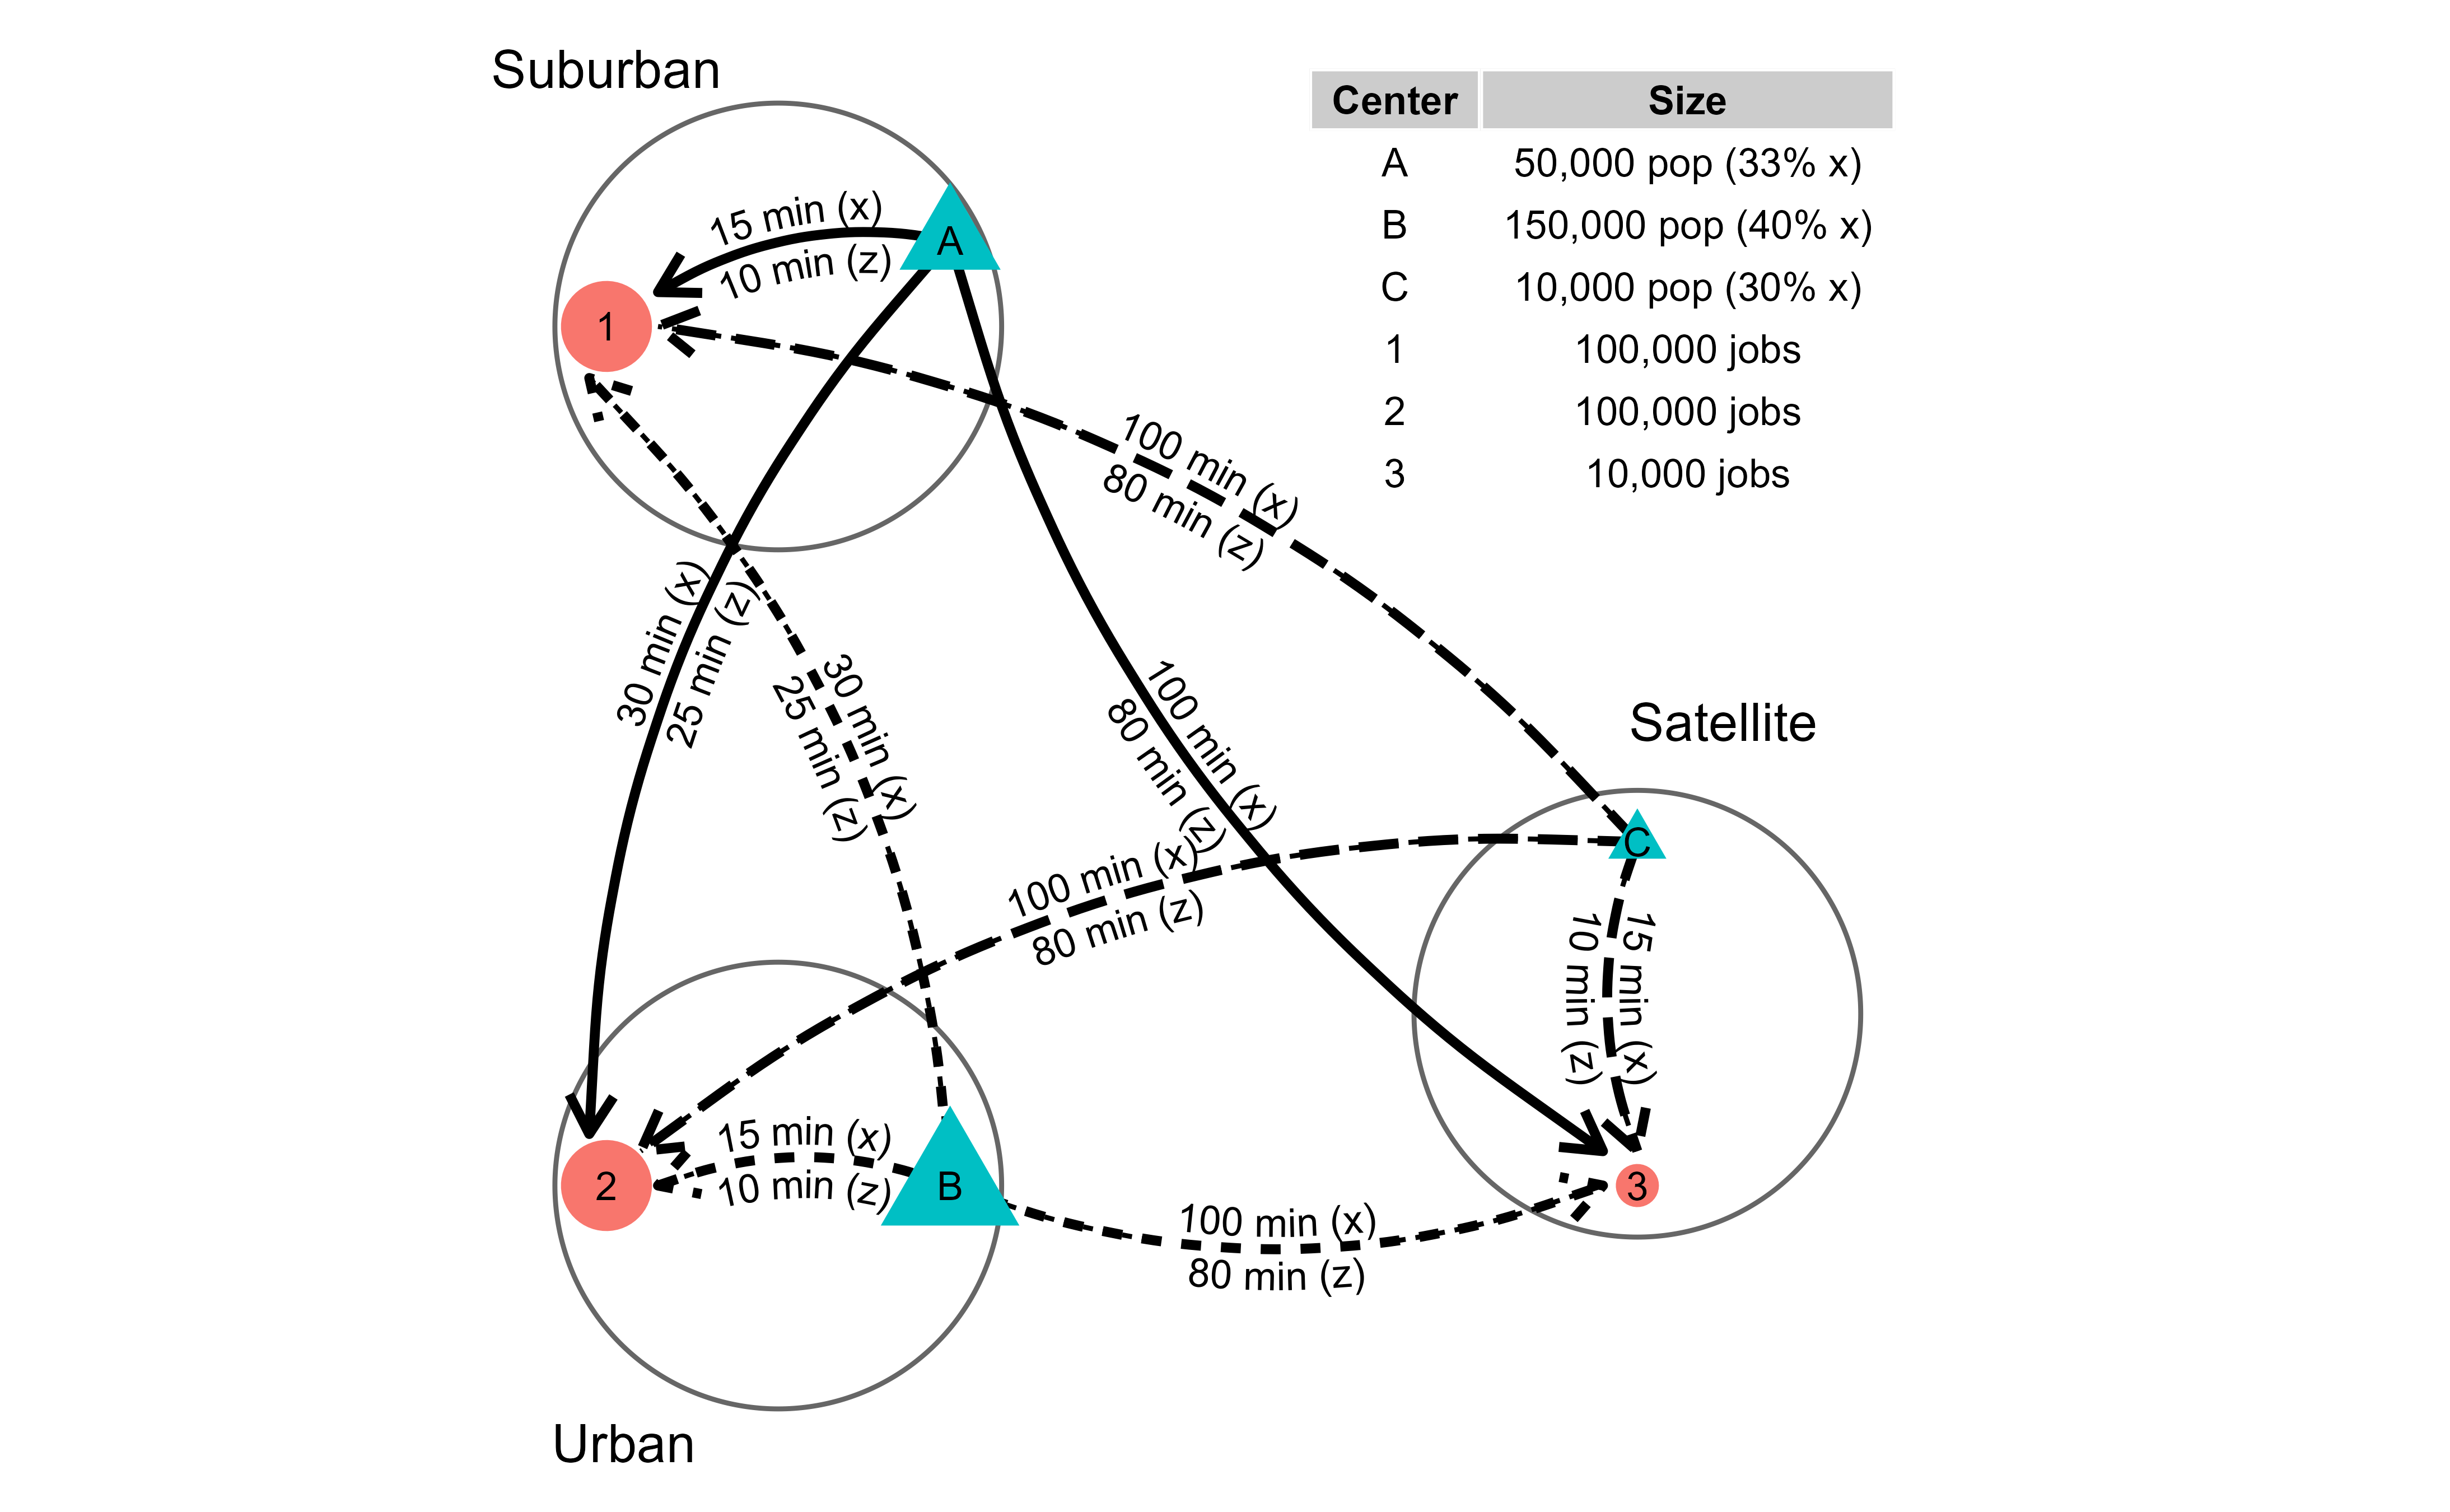
\includegraphics[width=1\linewidth]{images/Fig1} 
%DIFDELCMD < %%%
\DIFdelendFL \DIFaddbeginFL 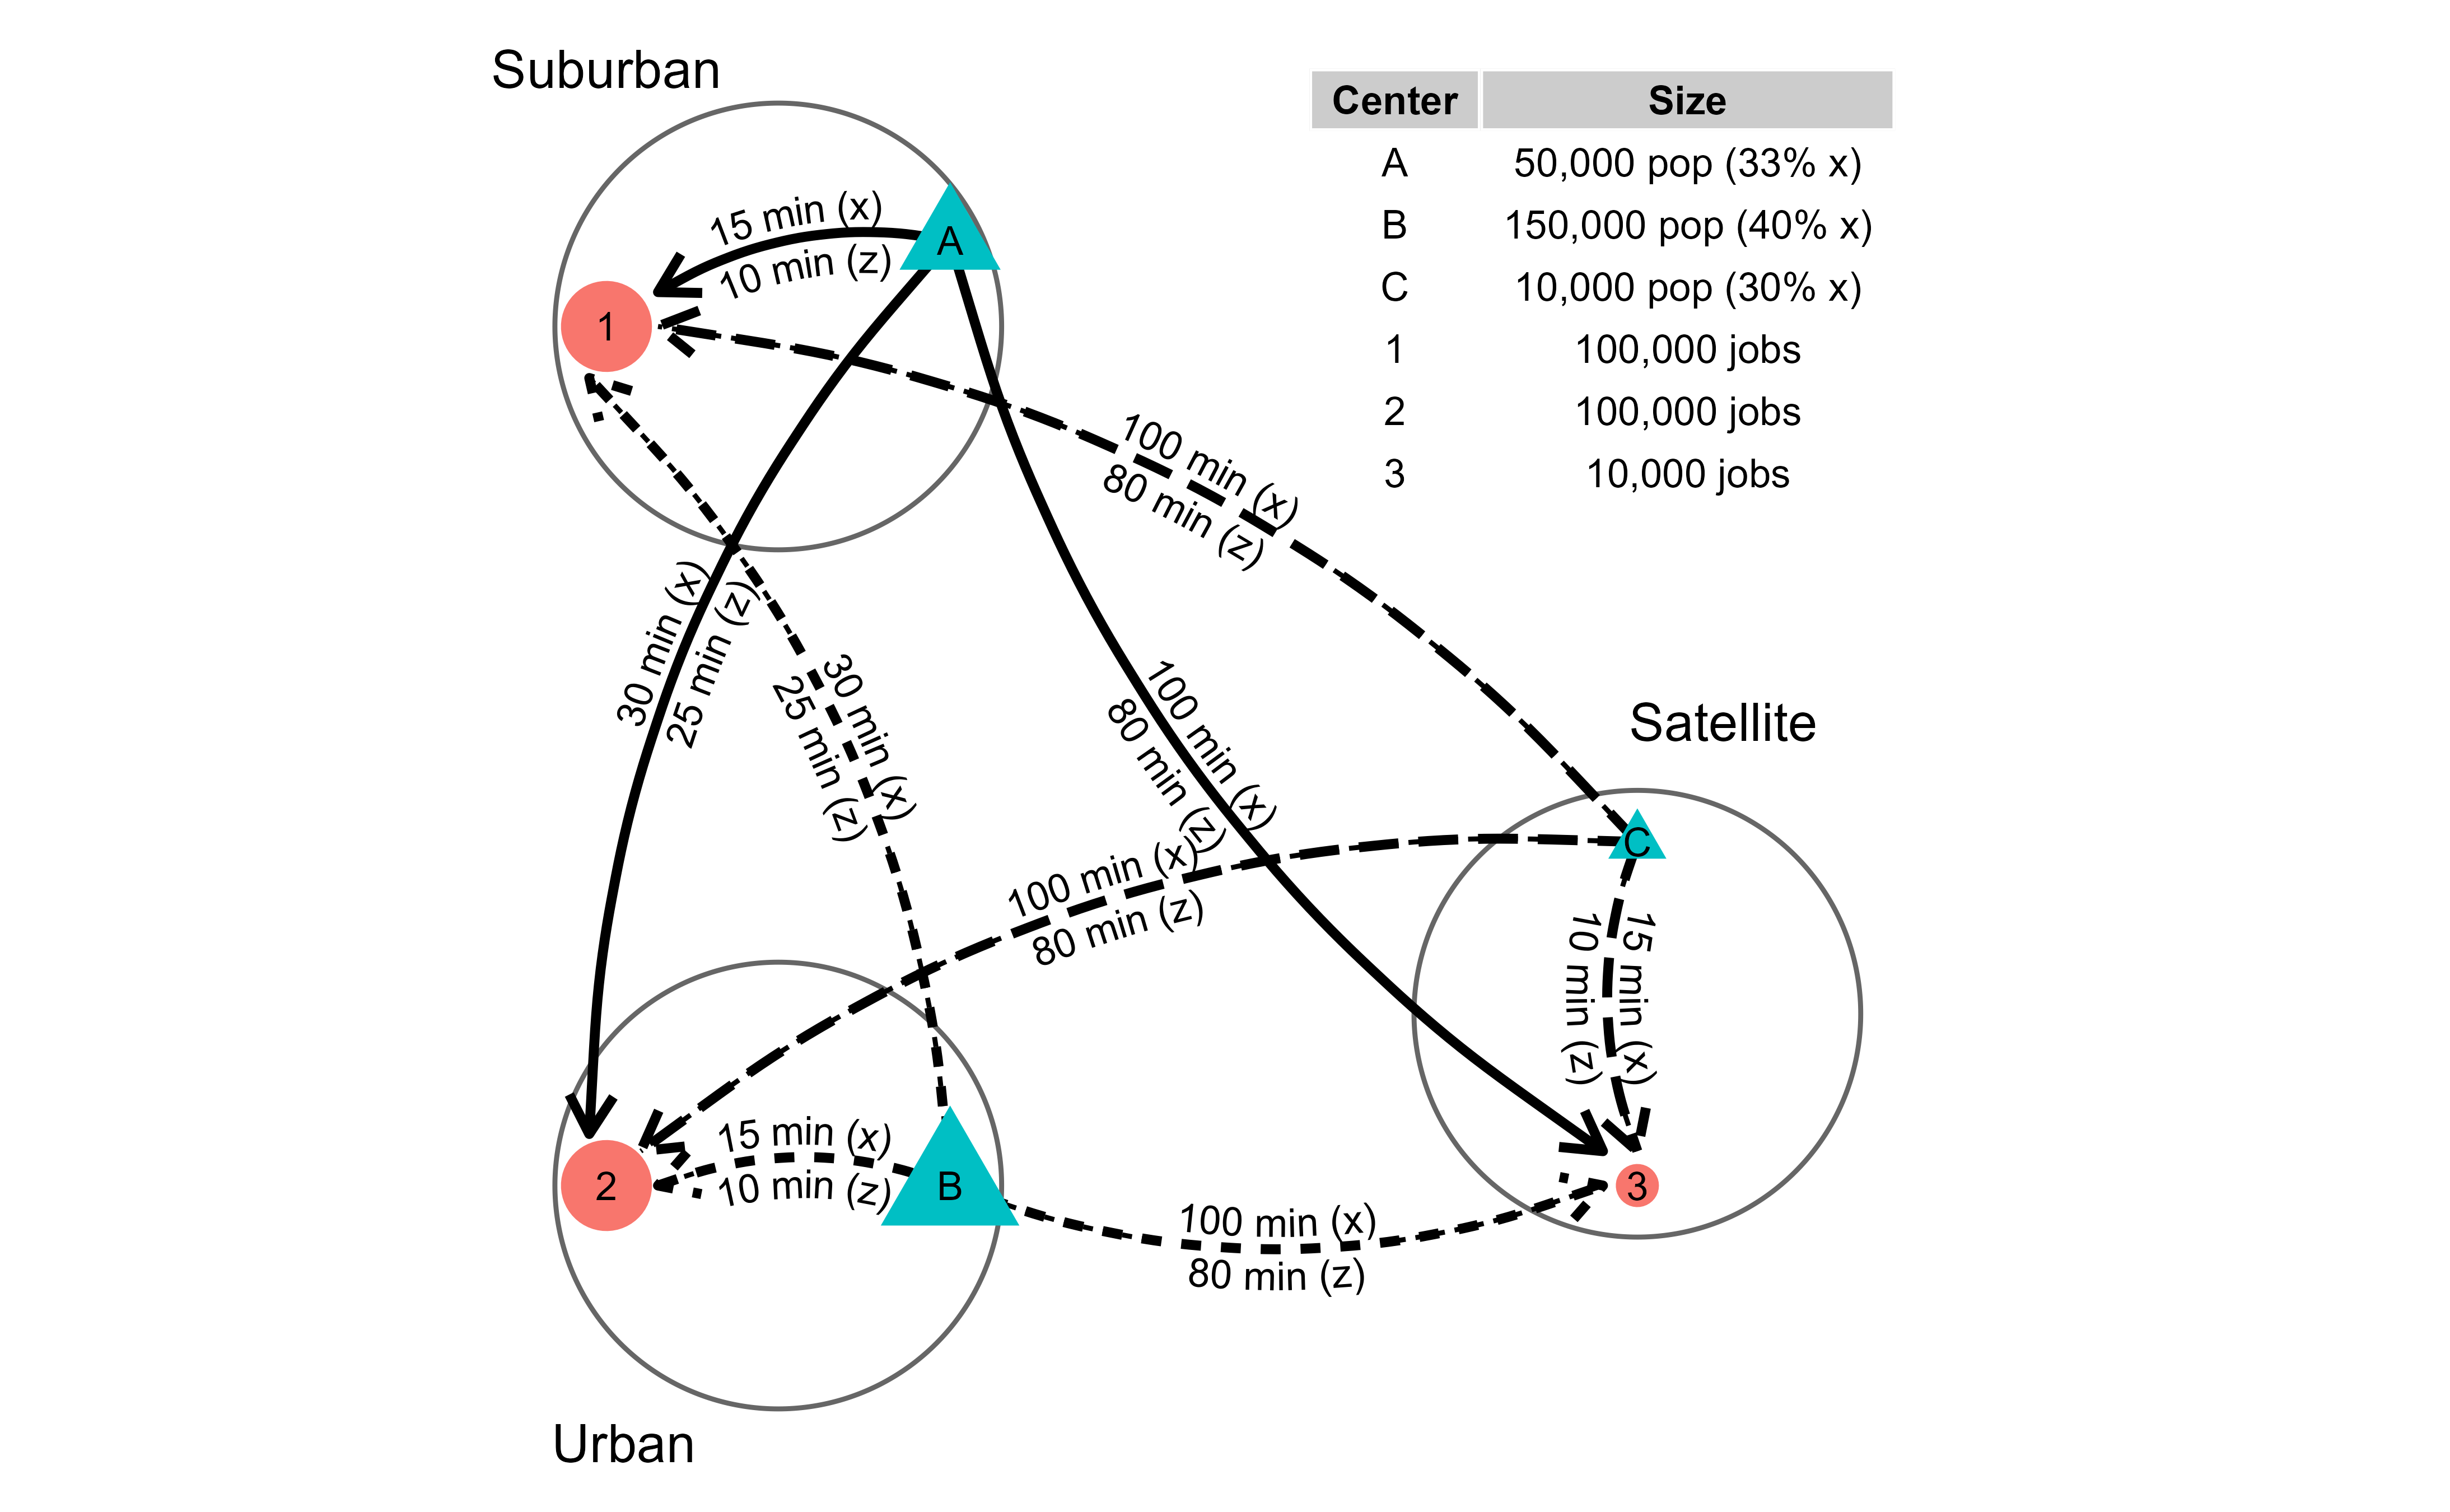
\includegraphics[width=0.85\linewidth]{images/Fig1} 
\DIFaddendFL 

}

\caption{\label{fig:Fig1} Multimodal synthetic example: locations of employment centers (in orange), population centers (in blue), number of jobs and population, and travel times for two modes (slower mode x and faster mode z).}\label{fig:synthetic-example-plot}
\end{figure}

From the perspective of access to a \emph{finite} amount of
opportunities in the region (\(210,000\) jobs), the sub-population that
is most proximate to jobs \DIFaddbegin \DIFadd{(low cost to reach)}\DIFaddend , furthest from \DIFdelbegin \DIFdel{densely populated centers, and is using the lowest travel-cost }\DIFdelend \DIFaddbegin \DIFadd{large
populations (less competition), and uses the fastest }\DIFaddend mode \(z\) \DIFdelbegin \DIFdel{can potentially access the most job }\DIFdelend \DIFaddbegin \DIFadd{(greater
range) can potentially reach the largest number of }\DIFaddend opportunities. This
appears to be the sub-population at \(A\) using \DIFaddbegin \DIFadd{mode }\DIFaddend \(z\).
\DIFdelbegin \DIFdel{From the other perspective, sub-populations }\DIFdelend \DIFaddbegin \DIFadd{Sub-populations }\DIFaddend located in opposite conditions (i.e., \DIFdelbegin \DIFdel{further away }\DIFdelend \DIFaddbegin \DIFadd{more distant }\DIFaddend from
jobs, close to \DIFdelbegin \DIFdel{dense
}\DIFdelend \DIFaddbegin \DIFadd{large }\DIFaddend populations, and using \DIFaddbegin \DIFadd{slow mode }\DIFaddend \(x\)) are at a
relative \DIFdelbegin \DIFdel{job opportunity access
}\emph{\DIFdel{disadvantage}}%DIFAUXCMD
\DIFdel{. From the perspective of inequities, the }\DIFdelend \DIFaddbegin \DIFadd{disadvantage. The }\DIFaddend competition for opportunities between
different mode-using populations matters as it reflects how well the
land-use and transport system serves (or \DIFdelbegin \DIFdel{doesn't
serve) them}\DIFdelend \DIFaddbegin \DIFadd{does not serve) certain
populations}\DIFaddend .

\global\setlength{\Oldarrayrulewidth}{\arrayrulewidth}

\global\setlength{\Oldtabcolsep}{\tabcolsep}

\setlength{\tabcolsep}{0pt}

\renewcommand*{\arraystretch}{1.5}



\providecommand{\ascline}[3]{\noalign{\global\arrayrulewidth #1}\arrayrulecolor[HTML]{#2}\cline{#3}}

\begin{longtable}[c]{|p{0.88in}|p{0.41in}|p{1.05in}|p{0.58in}|p{1.05in}|p{0.58in}|p{1.05in}}

\caption{Accessibility\ values\ at\ each\ origin\ \DIFaddbegin \DIFadd{(i)\ }\DIFaddend per\ mode\ \DIFaddbegin \DIFadd{(}\DIFaddend m\DIFaddbegin \DIFadd{)}\DIFaddend \ \DIFdelbegin \DIFdel{at}\DIFdelend \DIFaddbegin \DIFadd{(columns}\DIFaddend \ \DIFdelbegin \DIFdel{each}\DIFdelend \DIFaddbegin \DIFadd{three}\DIFaddend \ \DIFdelbegin \DIFdel{origin}\DIFdelend \DIFaddbegin \DIFadd{to}\DIFaddend \ \DIFdelbegin \DIFdel{i}\DIFdelend \DIFaddbegin \DIFadd{five)}\DIFaddend \ and\ aggregated\ \DIFdelbegin \DIFdel{between}\DIFdelend \DIFaddbegin \DIFadd{per}\DIFaddend \ \DIFdelbegin \DIFdel{modes}\DIFdelend \DIFaddbegin \DIFadd{i}\DIFaddend \ \DIFdelbegin \DIFdel{for}\DIFdelend \DIFaddbegin \DIFadd{(columns}\DIFaddend \ \DIFdelbegin \DIFdel{each}\DIFdelend \DIFaddbegin \DIFadd{six}\DIFaddend \ \DIFdelbegin \DIFdel{i}\DIFdelend \DIFaddbegin \DIFadd{and}\DIFaddend \ \DIFaddbegin \DIFadd{seven)\ }\DIFaddend for\ the\ synthetic\ example.}\\

\ascline{1.5pt}{666666}{1-7}

\multicolumn{1}{>{\raggedright}m{\dimexpr 0.88in+0\tabcolsep}}{\textcolor[HTML]{000000}{\fontsize{11}{11}\selectfont{i}}} & \multicolumn{1}{>{\raggedright}m{\dimexpr 0.41in+0\tabcolsep}}{\textcolor[HTML]{000000}{\fontsize{11}{11}\selectfont{m}}} & \multicolumn{1}{!{\color[HTML]{666666}\vrule width 1pt}>{\raggedleft}m{\dimexpr 1.05in+0\tabcolsep}}{\textcolor[HTML]{000000}{\fontsize{11}{11}\selectfont{S}}\textcolor[HTML]{000000}{\textsubscript{\fontsize{11}{11}\selectfont{i}}}\textcolor[HTML]{000000}{\textsuperscript{\fontsize{11}{11}\selectfont{m}}}} & \multicolumn{1}{>{\raggedleft}m{\dimexpr 0.58in+0\tabcolsep}}{\textcolor[HTML]{000000}{\fontsize{11}{11}\selectfont{a}}\textcolor[HTML]{000000}{\textsubscript{\fontsize{11}{11}\selectfont{i}}}\textcolor[HTML]{000000}{\textsuperscript{\fontsize{11}{11}\selectfont{m}}}} & \multicolumn{1}{>{\raggedleft}m{\dimexpr 1.05in+0\tabcolsep}}{\textcolor[HTML]{000000}{\fontsize{11}{11}\selectfont{V}}\textcolor[HTML]{000000}{\textsubscript{\fontsize{11}{11}\selectfont{i}}}\textcolor[HTML]{000000}{\textsuperscript{\fontsize{11}{11}\selectfont{m}}}} & \multicolumn{1}{!{\color[HTML]{666666}\vrule width 1pt}>{\raggedleft}m{\dimexpr 0.58in+0\tabcolsep}}{\textcolor[HTML]{000000}{\fontsize{11}{11}\selectfont{a}}\textcolor[HTML]{000000}{\textsubscript{\fontsize{11}{11}\selectfont{i}}}} & \multicolumn{1}{>{\raggedleft}m{\dimexpr 1.05in+0\tabcolsep}}{\textcolor[HTML]{000000}{\fontsize{11}{11}\selectfont{V}}\textcolor[HTML]{000000}{\textsubscript{\fontsize{11}{11}\selectfont{i}}}} \\

\ascline{1.5pt}{666666}{1-7}\endfirsthead \caption[]{Accessibility\ values\ at\ each\ origin\ \DIFaddbegin \DIFadd{(i)\ }\DIFaddend per\ mode\ \DIFaddbegin \DIFadd{(}\DIFaddend m\DIFaddbegin \DIFadd{)}\DIFaddend \ \DIFdelbegin \DIFdel{at}\DIFdelend \DIFaddbegin \DIFadd{(columns}\DIFaddend \ \DIFdelbegin \DIFdel{each}\DIFdelend \DIFaddbegin \DIFadd{three}\DIFaddend \ \DIFdelbegin \DIFdel{origin}\DIFdelend \DIFaddbegin \DIFadd{to}\DIFaddend \ \DIFdelbegin \DIFdel{i}\DIFdelend \DIFaddbegin \DIFadd{five)}\DIFaddend \ and\ aggregated\ \DIFdelbegin \DIFdel{between}\DIFdelend \DIFaddbegin \DIFadd{per}\DIFaddend \ \DIFdelbegin \DIFdel{modes}\DIFdelend \DIFaddbegin \DIFadd{i}\DIFaddend \ \DIFdelbegin \DIFdel{for}\DIFdelend \DIFaddbegin \DIFadd{(columns}\DIFaddend \ \DIFdelbegin \DIFdel{each}\DIFdelend \DIFaddbegin \DIFadd{six}\DIFaddend \ \DIFdelbegin \DIFdel{i}\DIFdelend \DIFaddbegin \DIFadd{and}\DIFaddend \ \DIFaddbegin \DIFadd{seven)\ }\DIFaddend for\ the\ synthetic\ example.}\\

\ascline{1.5pt}{666666}{1-7}

\multicolumn{1}{>{\raggedright}m{\dimexpr 0.88in+0\tabcolsep}}{\textcolor[HTML]{000000}{\fontsize{11}{11}\selectfont{i}}} & \multicolumn{1}{>{\raggedright}m{\dimexpr 0.41in+0\tabcolsep}}{\textcolor[HTML]{000000}{\fontsize{11}{11}\selectfont{m}}} & \multicolumn{1}{!{\color[HTML]{666666}\vrule width 1pt}>{\raggedleft}m{\dimexpr 1.05in+0\tabcolsep}}{\textcolor[HTML]{000000}{\fontsize{11}{11}\selectfont{S}}\textcolor[HTML]{000000}{\textsubscript{\fontsize{11}{11}\selectfont{i}}}\textcolor[HTML]{000000}{\textsuperscript{\fontsize{11}{11}\selectfont{m}}}} & \multicolumn{1}{>{\raggedleft}m{\dimexpr 0.58in+0\tabcolsep}}{\textcolor[HTML]{000000}{\fontsize{11}{11}\selectfont{a}}\textcolor[HTML]{000000}{\textsubscript{\fontsize{11}{11}\selectfont{i}}}\textcolor[HTML]{000000}{\textsuperscript{\fontsize{11}{11}\selectfont{m}}}} & \multicolumn{1}{>{\raggedleft}m{\dimexpr 1.05in+0\tabcolsep}}{\textcolor[HTML]{000000}{\fontsize{11}{11}\selectfont{V}}\textcolor[HTML]{000000}{\textsubscript{\fontsize{11}{11}\selectfont{i}}}\textcolor[HTML]{000000}{\textsuperscript{\fontsize{11}{11}\selectfont{m}}}} & \multicolumn{1}{!{\color[HTML]{666666}\vrule width 1pt}>{\raggedleft}m{\dimexpr 0.58in+0\tabcolsep}}{\textcolor[HTML]{000000}{\fontsize{11}{11}\selectfont{a}}\textcolor[HTML]{000000}{\textsubscript{\fontsize{11}{11}\selectfont{i}}}} & \multicolumn{1}{>{\raggedleft}m{\dimexpr 1.05in+0\tabcolsep}}{\textcolor[HTML]{000000}{\fontsize{11}{11}\selectfont{V}}\textcolor[HTML]{000000}{\textsubscript{\fontsize{11}{11}\selectfont{i}}}} \\

\ascline{1.5pt}{666666}{1-7}\endhead



\multicolumn{1}{>{\raggedright}m{\dimexpr 0.88in+0\tabcolsep}}{} & \multicolumn{1}{>{\raggedright}m{\dimexpr 0.41in+0\tabcolsep}}{\textcolor[HTML]{000000}{\fontsize{11}{11}\selectfont{x}}} & \multicolumn{1}{!{\color[HTML]{666666}\vrule width 1pt}>{\raggedleft}m{\dimexpr 1.05in+0\tabcolsep}}{\textcolor[HTML]{000000}{\fontsize{11}{11}\selectfont{27,292.18}}} & \multicolumn{1}{>{\raggedleft}m{\dimexpr 0.58in+0\tabcolsep}}{\textcolor[HTML]{000000}{\fontsize{11}{11}\selectfont{0.95}}} & \multicolumn{1}{>{\raggedleft}m{\dimexpr 1.05in+0\tabcolsep}}{\textcolor[HTML]{000000}{\fontsize{11}{11}\selectfont{15,696.89}}} & \multicolumn{1}{!{\color[HTML]{666666}\vrule width 1pt}>{\raggedleft}m{\dimexpr 0.58in+0\tabcolsep}}{} & \multicolumn{1}{>{\raggedleft}m{\dimexpr 1.05in+0\tabcolsep}}{} \\





\multicolumn{1}{>{\raggedright}m{\dimexpr 0.88in+0\tabcolsep}}{\multirow[c]{-2}{*}{\parbox{0.88in}{\raggedright \textcolor[HTML]{000000}{\fontsize{11}{11}\selectfont{A}}}}} & \multicolumn{1}{>{\raggedright}m{\dimexpr 0.41in+0\tabcolsep}}{\textcolor[HTML]{000000}{\fontsize{11}{11}\selectfont{z}}} & \multicolumn{1}{!{\color[HTML]{666666}\vrule width 1pt}>{\raggedleft}m{\dimexpr 1.05in+0\tabcolsep}}{\textcolor[HTML]{000000}{\fontsize{11}{11}\selectfont{44,999.80}}} & \multicolumn{1}{>{\raggedleft}m{\dimexpr 0.58in+0\tabcolsep}}{\textcolor[HTML]{000000}{\fontsize{11}{11}\selectfont{1.57}}} & \multicolumn{1}{>{\raggedleft}m{\dimexpr 1.05in+0\tabcolsep}}{\textcolor[HTML]{000000}{\fontsize{11}{11}\selectfont{51,785.72}}} & \multicolumn{1}{!{\color[HTML]{666666}\vrule width 1pt}>{\raggedleft}m{\dimexpr 0.58in+0\tabcolsep}}{\multirow[c]{-2}{*}{\parbox{0.58in}{\raggedleft \textcolor[HTML]{000000}{\fontsize{11}{11}\selectfont{1.36}}}}} & \multicolumn{1}{>{\raggedleft}m{\dimexpr 1.05in+0\tabcolsep}}{\multirow[c]{-2}{*}{\parbox{1.05in}{\raggedleft \textcolor[HTML]{000000}{\fontsize{11}{11}\selectfont{67,482.61}}}}} \\

\ascline{1pt}{666666}{1-7}



\multicolumn{1}{>{\raggedright}m{\dimexpr 0.88in+0\tabcolsep}}{} & \multicolumn{1}{>{\raggedright}m{\dimexpr 0.41in+0\tabcolsep}}{\textcolor[HTML]{000000}{\fontsize{11}{11}\selectfont{x}}} & \multicolumn{1}{!{\color[HTML]{666666}\vrule width 1pt}>{\raggedleft}m{\dimexpr 1.05in+0\tabcolsep}}{\textcolor[HTML]{000000}{\fontsize{11}{11}\selectfont{27,292.18}}} & \multicolumn{1}{>{\raggedleft}m{\dimexpr 0.58in+0\tabcolsep}}{\textcolor[HTML]{000000}{\fontsize{11}{11}\selectfont{0.64}}} & \multicolumn{1}{>{\raggedleft}m{\dimexpr 1.05in+0\tabcolsep}}{\textcolor[HTML]{000000}{\fontsize{11}{11}\selectfont{38,170.03}}} & \multicolumn{1}{!{\color[HTML]{666666}\vrule width 1pt}>{\raggedleft}m{\dimexpr 0.58in+0\tabcolsep}}{} & \multicolumn{1}{>{\raggedleft}m{\dimexpr 1.05in+0\tabcolsep}}{} \\





\multicolumn{1}{>{\raggedright}m{\dimexpr 0.88in+0\tabcolsep}}{\multirow[c]{-2}{*}{\parbox{0.88in}{\raggedright \textcolor[HTML]{000000}{\fontsize{11}{11}\selectfont{B}}}}} & \multicolumn{1}{>{\raggedright}m{\dimexpr 0.41in+0\tabcolsep}}{\textcolor[HTML]{000000}{\fontsize{11}{11}\selectfont{z}}} & \multicolumn{1}{!{\color[HTML]{666666}\vrule width 1pt}>{\raggedleft}m{\dimexpr 1.05in+0\tabcolsep}}{\textcolor[HTML]{000000}{\fontsize{11}{11}\selectfont{44,999.80}}} & \multicolumn{1}{>{\raggedleft}m{\dimexpr 0.58in+0\tabcolsep}}{\textcolor[HTML]{000000}{\fontsize{11}{11}\selectfont{1.05}}} & \multicolumn{1}{>{\raggedleft}m{\dimexpr 1.05in+0\tabcolsep}}{\textcolor[HTML]{000000}{\fontsize{11}{11}\selectfont{94,468.91}}} & \multicolumn{1}{!{\color[HTML]{666666}\vrule width 1pt}>{\raggedleft}m{\dimexpr 0.58in+0\tabcolsep}}{\multirow[c]{-2}{*}{\parbox{0.58in}{\raggedleft \textcolor[HTML]{000000}{\fontsize{11}{11}\selectfont{0.88}}}}} & \multicolumn{1}{>{\raggedleft}m{\dimexpr 1.05in+0\tabcolsep}}{\multirow[c]{-2}{*}{\parbox{1.05in}{\raggedleft \textcolor[HTML]{000000}{\fontsize{11}{11}\selectfont{132,638.94}}}}} \\

\ascline{1pt}{666666}{1-7}



\multicolumn{1}{>{\raggedright}m{\dimexpr 0.88in+0\tabcolsep}}{} & \multicolumn{1}{>{\raggedright}m{\dimexpr 0.41in+0\tabcolsep}}{\textcolor[HTML]{000000}{\fontsize{11}{11}\selectfont{x}}} & \multicolumn{1}{!{\color[HTML]{666666}\vrule width 1pt}>{\raggedleft}m{\dimexpr 1.05in+0\tabcolsep}}{\textcolor[HTML]{000000}{\fontsize{11}{11}\selectfont{2,240.38}}} & \multicolumn{1}{>{\raggedleft}m{\dimexpr 0.58in+0\tabcolsep}}{\textcolor[HTML]{000000}{\fontsize{11}{11}\selectfont{0.68}}} & \multicolumn{1}{>{\raggedleft}m{\dimexpr 1.05in+0\tabcolsep}}{\textcolor[HTML]{000000}{\fontsize{11}{11}\selectfont{2,035.86}}} & \multicolumn{1}{!{\color[HTML]{666666}\vrule width 1pt}>{\raggedleft}m{\dimexpr 0.58in+0\tabcolsep}}{} & \multicolumn{1}{>{\raggedleft}m{\dimexpr 1.05in+0\tabcolsep}}{} \\





\multicolumn{1}{>{\raggedright}m{\dimexpr 0.88in+0\tabcolsep}}{\multirow[c]{-2}{*}{\parbox{0.88in}{\raggedright \textcolor[HTML]{000000}{\fontsize{11}{11}\selectfont{C}}}}} & \multicolumn{1}{>{\raggedright}m{\dimexpr 0.41in+0\tabcolsep}}{\textcolor[HTML]{000000}{\fontsize{11}{11}\selectfont{z}}} & \multicolumn{1}{!{\color[HTML]{666666}\vrule width 1pt}>{\raggedleft}m{\dimexpr 1.05in+0\tabcolsep}}{\textcolor[HTML]{000000}{\fontsize{11}{11}\selectfont{3,745.89}}} & \multicolumn{1}{>{\raggedleft}m{\dimexpr 0.58in+0\tabcolsep}}{\textcolor[HTML]{000000}{\fontsize{11}{11}\selectfont{1.12}}} & \multicolumn{1}{>{\raggedleft}m{\dimexpr 1.05in+0\tabcolsep}}{\textcolor[HTML]{000000}{\fontsize{11}{11}\selectfont{7,842.59}}} & \multicolumn{1}{!{\color[HTML]{666666}\vrule width 1pt}>{\raggedleft}m{\dimexpr 0.58in+0\tabcolsep}}{\multirow[c]{-2}{*}{\parbox{0.58in}{\raggedleft \textcolor[HTML]{000000}{\fontsize{11}{11}\selectfont{0.99}}}}} & \multicolumn{1}{>{\raggedleft}m{\dimexpr 1.05in+0\tabcolsep}}{\multirow[c]{-2}{*}{\parbox{1.05in}{\raggedleft \textcolor[HTML]{000000}{\fontsize{11}{11}\selectfont{9,878.45}}}}} \\

\ascline{1pt}{666666}{1-7}



\multicolumn{1}{>{\raggedright}m{\dimexpr 0.88in+0\tabcolsep}}{\textcolor[HTML]{000000}{\fontsize{11}{11}\selectfont{TOTALS}}} & \multicolumn{1}{>{\raggedright}m{\dimexpr 0.41in+0\tabcolsep}}{\textcolor[HTML]{000000}{\fontsize{11}{11}\selectfont{}}} & \multicolumn{1}{!{\color[HTML]{666666}\vrule width 1pt}>{\raggedleft}m{\dimexpr 1.05in+0\tabcolsep}}{\textcolor[HTML]{000000}{\fontsize{11}{11}\selectfont{150,570.22}}} & \multicolumn{1}{>{\raggedleft}m{\dimexpr 0.58in+0\tabcolsep}}{\textcolor[HTML]{000000}{\fontsize{11}{11}\selectfont{N/A}}} & \multicolumn{1}{>{\raggedleft}m{\dimexpr 1.05in+0\tabcolsep}}{\textcolor[HTML]{000000}{\fontsize{11}{11}\selectfont{210,000.00}}} & \multicolumn{1}{!{\color[HTML]{666666}\vrule width 1pt}>{\raggedleft}m{\dimexpr 0.58in+0\tabcolsep}}{\textcolor[HTML]{000000}{\fontsize{11}{11}\selectfont{N/A}}} & \multicolumn{1}{>{\raggedleft}m{\dimexpr 1.05in+0\tabcolsep}}{\textcolor[HTML]{000000}{\fontsize{11}{11}\selectfont{210,000.00}}} \\

\ascline{1.5pt}{666666}{1-7}



\end{longtable}



\arrayrulecolor[HTML]{000000}

\global\setlength{\arrayrulewidth}{\Oldarrayrulewidth}

\global\setlength{\tabcolsep}{\Oldtabcolsep}

\renewcommand*{\arraystretch}{1}

The \DIFdelbegin \DIFdel{calculated }\DIFdelend \DIFaddbegin \DIFadd{values calculated for }\DIFaddend \(S_i^m\) \DIFaddbegin \DIFadd{(Hansen-type accessibility)}\DIFaddend ,
\(a_i^m\) \DIFaddbegin \DIFadd{(Shen-type accessibility), }\DIFaddend and \(V_i^m\) \DIFdelbegin \DIFdel{accessibility values
}\DIFdelend \DIFaddbegin \DIFadd{(spatial
availability) }\DIFaddend for each \(i\) and \(m\) are shown in the middle three
columns and are aggregated for each \(i\) in the final two columns in
Table 1 . \DIFdelbegin \DIFdel{We }\DIFdelend \DIFaddbegin \DIFadd{As in the example in Shen }{[}\DIFadd{12}{]}\DIFadd{, we }\DIFaddend use a negative
exponential impedance function
\DIFdelbegin \DIFdel{\(f(c_{ij}) = \exp(-\beta\cdot c_{ij})\) }\DIFdelend \DIFaddbegin \DIFadd{\(f^m(c_{ij}^m) = \exp(-\beta\cdot c_{ij})\) }\DIFaddend with \(\beta=0.1\) for both
\(x\) and \(z\) modes for all accessibility measures calculations.
\DIFaddbegin \DIFadd{Notice that in this example we use the same impedance function but the
travel times are different for the two modes. More generally, it is
possible to use different impedance functions for the modes, as
demonstrated in the empirical example in the following section.
}\DIFaddend 

\DIFdelbegin \DIFdel{The }\DIFdelend Hansen-type \DIFdelbegin \DIFdel{measure }\DIFdelend \DIFaddbegin \DIFadd{accessibility }\DIFaddend \(S_i^m\) is presented for each origin and
mode in \DIFaddbegin \DIFadd{the }\DIFaddend third column of Table 1 . For all \(i\), the \DIFaddbegin \DIFadd{travel by }\DIFaddend \(z\)
\DIFdelbegin \DIFdel{-using
sub-population has higher \(S_i^m\) values than the }\DIFdelend \DIFaddbegin \DIFadd{results in higher values of \(S_i^m\) than travel by }\DIFaddend \(x\)\DIFdelbegin \DIFdel{-using
sub-populations. Additionally, }\DIFdelend \DIFaddbegin \DIFadd{. Lack of
competition, or alternatively the assumption of an inexhaustible
resource in the calculation of }\DIFaddend \(S_i^m\)\DIFdelbegin \DIFdel{is equal for both mode-using
populations in \(A\) and \(B\). This is the case because \(S_i^m\) does
not consider }\emph{\DIFdel{competition}}%DIFAUXCMD
\DIFdel{, it only relies on reflecting the count
of opportunities that may be interacted with as a product of
\(f^m(c_{ij}^m)\).
Recall, }\DIFdelend \DIFaddbegin \DIFadd{, lead to a curious result.
Since the }\DIFaddend populations in \(A\) and \(B\) have the same travel impedance
to employment centers \(1\), \(2\) and \(3\) (either 15, 30, or 100
minutes using \(x\) or 10, 25, or 80 minutes using \(z\))\DIFdelbegin \DIFdel{. As such, these the calculated \(S_i^m\) values
}\DIFdelend \DIFaddbegin \DIFadd{, their values
of \(S_i^m\) }\DIFaddend are the same for both \(A\) and \(B\). Furthermore, the
total sum of \(S_i^m\) in the region is equal to 150,570.2. This value
\DIFdelbegin \DIFdel{is difficult to interpret}\DIFdelend \DIFaddbegin \DIFadd{lacks an intuitive interpretation}\DIFaddend : it represents the weighted sum of
opportunities that may be \DIFdelbegin \DIFdel{interacted with
}\DIFdelend \DIFaddbegin \DIFadd{reached }\DIFaddend within the region \DIFdelbegin \DIFdel{based on travel impedance . It cannot be interpreted as
}\DIFdelend \DIFaddbegin \DIFadd{according to the
travel impedance (i.e., the travel behavior and the characteristics of
the modes) and does not usefully translate into }\DIFaddend any sort of benchmark\DIFdelbegin \DIFdel{since the measure is }\emph{\DIFdel{non-constrained}}%DIFAUXCMD
\DIFdelend .
To connect this example to \DIFaddbegin \DIFadd{the aforementioned }\DIFaddend literature, \(S_i^m\) is
calculated in the work of \DIFaddbegin \DIFadd{Tahmasbi et al. }\DIFaddend {[}\DIFdelbegin \DIFdel{15}\DIFdelend \DIFaddbegin \DIFadd{21}\DIFaddend {]}; they \DIFdelbegin \DIFdel{compare }\DIFdelend \DIFaddbegin \DIFadd{contrast
}\DIFaddend differences in \(S_i^m\) values between modes in a relative and
comparative sense, but make no further interpretation of the \(S_i^m\)
values. \DIFaddbegin \DIFadd{More densely populated metropolitan regions will tend to have
more opportunities and hence large \(S_i^m\) values and less densely
regions, smaller values; how much of these differences may simply an
artifact of region density?
}\DIFaddend 

In the fourth and sixth \DIFdelbegin \DIFdel{column }\DIFdelend \DIFaddbegin \DIFadd{columns }\DIFaddend in Table 1 the \DIFaddbegin \DIFadd{results for }\DIFaddend Shen-type
\DIFdelbegin \DIFdel{measure is
calculated}\DIFdelend \DIFaddbegin \DIFadd{accessibility are reported}\DIFaddend : first for both origin and mode \(a_i^m\) as
well as aggregated by the weighted mean mode-population (
\(\sum_m \frac{P_i^m}{P_i}*a_i^m\) ) to represent a value for each
origin \(a_i\). Unlike \(S_i^m\), this measure \DIFaddbegin \DIFadd{does }\DIFaddend considers
\emph{competition}. For instance, the \DIFaddbegin \DIFadd{population travelling by }\DIFaddend \(x\)
\DIFdelbegin \DIFdel{-using populations in }\DIFdelend \DIFaddbegin \DIFadd{from }\DIFaddend \(A\) and \(B\) \DIFdelbegin \DIFdel{centers }\DIFdelend do not have the same \DIFdelbegin \DIFdel{\(a_i^m\) values as the
}\DIFdelend \DIFaddbegin \DIFadd{values of \(a_i^m\) as those
travelling by }\DIFaddend \(z\)\DIFdelbegin \DIFdel{-using}\DIFdelend . In fact, \(A\) has the highest values \(a_i^m\) and
\(a_i\) values since this center has the \DIFdelbegin \DIFdel{smallest }\DIFdelend \DIFaddbegin \DIFadd{lowest }\DIFaddend travel impedance to
opportunities (lower than at \(C\), \(A\) and \(B\) are equal) and \DIFdelbegin \DIFdel{has
one of these lowest proximity }\DIFdelend \DIFaddbegin \DIFadd{faces
relatively low competition, not being close }\DIFaddend to a relatively \DIFdelbegin \DIFdel{high amount of }\DIFdelend \DIFaddbegin \DIFadd{large
}\DIFaddend population (lower than at \(B\)).

However, the \DIFdelbegin \DIFdel{Shen-type measure is }\emph{\DIFdel{non-constrained}}%DIFAUXCMD
\DIFdelend \DIFaddbegin \DIFadd{calculations of \(a_i^m\) are not constrained}\DIFaddend : the total
sum of \(a_i^m\) or \(a_i\) is practically meaningless since it
represents a sum of ratios. For instance, the \DIFaddbegin \DIFadd{population travelling by
}\DIFaddend \(z\) \DIFdelbegin \DIFdel{-using sub-population at }\DIFdelend \DIFaddbegin \DIFadd{from }\DIFaddend \(A\) has a value of 1.57 \DIFdelbegin \DIFdel{potential jobs per potential }\DIFdelend \DIFaddbegin \DIFadd{jobs per }\DIFaddend job-seeking population
compared to 0.95 for \DIFaddbegin \DIFadd{users of mode }\DIFaddend \(x\)\DIFdelbegin \DIFdel{-using sub-population}\DIFdelend . What is the \DIFdelbegin \DIFdel{significance }\DIFdelend \DIFaddbegin \DIFadd{meaning }\DIFaddend of these
values? The difference between these modes is equal to 0.62, but 0.62 of
what? How many more job opportunities \DIFdelbegin \DIFdel{are
\(z\) users interacting with than }\DIFdelend \DIFaddbegin \DIFadd{can users of \(z\) reach compared
to user of }\DIFaddend \(x\)\DIFdelbegin \DIFdel{users}\DIFdelend ? When \(a_i^m\) is aggregated to \(a_i\) as shown in
the sixth column, the values face similar interpretability issues. The
Shen-type measure is implemented in \DIFdelbegin \DIFdel{the previously discussed work of }\DIFdelend \DIFaddbegin \DIFadd{aforementioned work of Tao et al.
}\DIFaddend {[}\DIFdelbegin \DIFdel{20}\DIFdelend \DIFaddbegin \DIFadd{36}\DIFaddend {]} to calculate modal \(a_i^m\) values and the aggregated \(a_i\)
is implemented in the work of \DIFaddbegin \DIFadd{Carpentier et al. }\DIFaddend {[}\DIFdelbegin \DIFdel{21}\DIFdelend \DIFaddbegin \DIFadd{38}\DIFaddend {]}. However,
similar to \DIFdelbegin \DIFdel{the }\DIFdelend Hansen-type \DIFdelbegin \DIFdel{measure}\DIFdelend \DIFaddbegin \DIFadd{accessibility}\DIFaddend , these works discuss relative and
spatially comparative differences in values, \DIFdelbegin \DIFdel{they
do not make further interpretation of the }\DIFdelend \DIFaddbegin \DIFadd{but veer from interpreting
the values of }\DIFaddend \(a_i^m\) or \(a_i\) themselves. \DIFdelbegin \DIFdel{This may be because the Shen-type measure is
}\emph{\DIFdel{non-constrained}}%DIFAUXCMD
\DIFdel{,
this is no benchmark or global maximum to which
comparisons can be drawn from}\DIFdelend \DIFaddbegin \DIFadd{In fairness,
interpretation is complicated by the multiple counting of opportunities
between zones and modes}\DIFaddend .

\DIFdelbegin \DIFdel{By }\DIFdelend \DIFaddbegin \DIFadd{In }\DIFaddend contrast, spatial availability \(V_i\) considers competition and is
constrained such that the total sum of values is equal to the total
number of opportunities in the region (i.e., \(210,000\) jobs). Seen in
fifth column of Table 1 , \DIFaddbegin \DIFadd{the values of }\DIFaddend \(V_i^m\) \DIFdelbegin \DIFdel{for the same mode-using populations
}\DIFdelend in \(A\) and \(B\) are
not the same \DIFaddbegin \DIFadd{within each mode }\DIFaddend (as this measure considers competition).
In fact, at \(A\), \DIFdelbegin \DIFdel{the }\DIFdelend \DIFaddbegin \DIFadd{users of mode }\DIFaddend \(z\) \DIFdelbegin \DIFdel{-using sub-population captures
}\DIFdelend \DIFaddbegin \DIFadd{capture }\DIFaddend 36,088.84 more spatially
available jobs (of the \(210,000\) jobs in the region) than the
sub-population \DIFdelbegin \DIFdel{using mode }\DIFdelend \DIFaddbegin \DIFadd{travelling by }\DIFaddend \(x\). The numerical difference \DIFdelbegin \DIFdel{has a practical interpretation}\DIFdelend \DIFaddbegin \DIFadd{is clear
since it refers to opportunities out of the total}\DIFaddend .

Furthermore, \DIFdelbegin \DIFdel{\(V_i^m\) values for an }\DIFdelend \DIFaddbegin \DIFadd{the proportional allocation mechanism also means that the
values of \(V_i^m\) for any origin }\DIFaddend \(i\) can be aggregated across \(m\)
and compared \DIFdelbegin \DIFdel{across \(i\) }\DIFdelend \DIFaddbegin \DIFadd{between zones }\DIFaddend (\(V_i = \sum_m{\sum_i{V_i^m}}\))\DIFdelbegin \DIFdel{as a
result of the proportional allocation mechanism}\DIFdelend . This
aggregation, \(V_i\), is shown in the seventh column in Table 1 . Again
looking at center \(A\), \(A\) is allocated 67,482.61 spatially
available opportunities for both modes. 77\% of this spatial
availability allocated to \(A\) is assigned to \DIFdelbegin \DIFdel{the }\DIFdelend \DIFaddbegin \DIFadd{users of mode }\DIFaddend \(z\)
\DIFdelbegin \DIFdel{-using population }\DIFdelend despite representing 66\% of \(A\)'s population.

Spatial availability can be further aggregated to better interpret
competition between modes. Across the entire region, 130,000 people use
\(z\) (62\% of the region population). However, \DIFdelbegin \DIFdel{the }\DIFdelend \DIFaddbegin \DIFadd{users of }\DIFaddend \(z\) \DIFdelbegin \DIFdel{-using
population accounts }\DIFdelend \DIFaddbegin \DIFadd{account
}\DIFaddend for 73\% of the region's total spatial availability - \DIFdelbegin \DIFdel{the rest }\DIFdelend \DIFaddbegin \DIFadd{while the
remaining 27\% }\DIFaddend is allocated to \DIFdelbegin \DIFdel{the }\DIFdelend \DIFaddbegin \DIFadd{users of mode }\DIFaddend \(x\) \DIFdelbegin \DIFdel{-using population (}\DIFdelend \DIFaddbegin \DIFadd{who are }\DIFaddend 38\%of the
total population\DIFdelbegin \DIFdel{)}\DIFdelend . Notably, the \DIFaddbegin \DIFadd{population who uses }\DIFaddend \(x\) \DIFdelbegin \DIFdel{-using population captures }\DIFdelend \DIFaddbegin \DIFadd{have }\DIFaddend 11\% \DIFdelbegin \DIFdel{less
spatial availability to }\DIFdelend \DIFaddbegin \DIFadd{fewer
spatially available }\DIFaddend opportunities than its \DIFdelbegin \DIFdel{population proportion. This
understanding can lead }\DIFdelend \DIFaddbegin \DIFadd{share in the population. This
realization leads }\DIFaddend us to ask normative questions such as, how unequal
should \DIFdelbegin \DIFdel{opportunity access for the two mode-using populations be }\DIFdelend \DIFaddbegin \DIFadd{availability of opportunities be by mode? What intervention could
help to redistribute spatial availability to sub-populations
commensurate with their proportion of the total}\DIFaddend ?
\DIFdelbegin \DIFdel{Can the lower-travel-cost populations spare some spatial availability if
a policy of modal-restriction (like a LEZ) was introduced?
}\DIFdelend 

Since spatial availability is constrained and has an interpretable
meaning as a proportion of the total opportunities in the region, the
values at \(i\) have a \DIFdelbegin \DIFdel{new significance}\DIFdelend \DIFaddbegin \DIFadd{straighforward interpretation}\DIFaddend . Inequality in
\(V_i^m\) values can be explored through a variety of approaches. For
instance, consider travel times. The \DIFaddbegin \DIFadd{population of travelers who use
}\DIFaddend \(z\) \DIFdelbegin \DIFdel{-using population }\DIFdelend accounts for 67\% of the potential travel time traveled in the
region: this is 7\% less travel time than the proportion of spatial
available opportunities that is allocated to them. In other words, the
\DIFdelbegin \DIFdel{\(z\)-using population travels
less }\DIFdelend \DIFaddbegin \DIFadd{population of users of \(z\) travels fewer }\DIFaddend minutes overall and has more
spatial availability of opportunities than \DIFdelbegin \DIFdel{the \(x\)-using population using the }\DIFdelend \DIFaddbegin \DIFadd{users of the }\DIFaddend slower mode
\(x\).

Alternatively, inequities in spatial availability between \DIFdelbegin \DIFdel{mode-using
populations }\DIFdelend \DIFaddbegin \DIFadd{modes }\DIFaddend can be
explored through proportional benchmarks. A spatial availability per
capita \(v_i^m\) \DIFdelbegin \DIFdel{as }\DIFdelend \DIFaddbegin \DIFadd{is }\DIFaddend presented in Equation (\ref{eq:SA-per-capita}):

\begin{equation}
\label{eq:SA-per-capita}
v_{i}^m = \frac{V_{i}^m}{P_{i}^m}
\end{equation}

The \DIFdelbegin \DIFdel{\(v_i^m\) values }\DIFdelend \DIFaddbegin \DIFadd{values of \(v_i^m\) }\DIFaddend for \(A\), \(B\), and \(C\) for \DIFdelbegin \DIFdel{the }\DIFdelend \DIFaddbegin \DIFadd{users of }\DIFaddend \(x\)
\DIFdelbegin \DIFdel{-using
sub-populations }\DIFdelend are 0.95, 0.64 and 0.68 spatially available jobs per capita,
respectively. The \DIFaddbegin \DIFadd{values of }\DIFaddend \(v_i^m\) for \DIFdelbegin \DIFdel{the }\DIFdelend \DIFaddbegin \DIFadd{users of }\DIFaddend \(z\) \DIFdelbegin \DIFdel{-using sub-populations
}\DIFdelend are much
higher, with values of: 1.57, 1.05 and 1.12 respectively. \DIFdelbegin \DIFdel{The
}\DIFdelend \DIFaddbegin \DIFadd{Users of
}\DIFaddend \(x\)\DIFdelbegin \DIFdel{-using population, especially }\DIFdelend \DIFaddbegin \DIFadd{, especially those }\DIFaddend at \(B\) and \(C\), are directly impacted by the
jobs that are spatially available to \DIFdelbegin \DIFdel{the }\DIFdelend \DIFaddbegin \DIFadd{users of }\DIFaddend \(z\) \DIFdelbegin \DIFdel{-using
population }\DIFdelend \emph{in addition
to} the mass effect (occurring at \(B\), high population density) and
high travel impedance (occurring at the Satellite \(C\)).

If, \DIFdelbegin \DIFdel{lets }\DIFdelend \DIFaddbegin \DIFadd{let us }\DIFaddend say, the planning goal \DIFdelbegin \DIFdel{is }\DIFdelend \DIFaddbegin \DIFadd{was }\DIFaddend to have one spatially available
job per mode-using population, a policy intervention \DIFdelbegin \DIFdel{can be put in place}\DIFdelend \DIFaddbegin \DIFadd{could be devised}\DIFaddend ,
to reduce the \DIFdelbegin \DIFdel{\(v_i^z\) values and increase \(v_i^x\) values . This
}\DIFdelend \DIFaddbegin \DIFadd{values of \(v_i^z\) (making it slower or more expensive)
and increase he values of \(v_i^x\) (making it faster or les expensive).
The purpose of this simple }\DIFaddend demonstration is to show how \DIFdelbegin \DIFdel{simply the \(V_i^m\) framework can be manipulated }\DIFdelend \DIFaddbegin \DIFadd{spatial
availability can be used to }\DIFaddend quantify the competitive (dis)advantage in a
multimodal application. In what follows, we \DIFdelbegin \DIFdel{further explore competition between
multiple modes }\DIFdelend \DIFaddbegin \DIFadd{demonstrate the use of
multimodal spatial availability }\DIFaddend through an empirical example.

\DIFdelbegin %DIFDELCMD < \hypertarget{empirical-example-madrid-lez}{%
%DIFDELCMD < \section{Empirical example: Madrid
%DIFDELCMD < LEZ}\label{empirical-example-madrid-lez}}
%DIFDELCMD < %%%
\DIFdelend \DIFaddbegin \hypertarget{empirical-example}{%
\section{Empirical example}\label{empirical-example}}
\DIFaddend 

\DIFdelbegin %DIFDELCMD < \hypertarget{multimodal-data-and-methods}{%
%DIFDELCMD < \subsection{Multimodal data and
%DIFDELCMD < methods}\label{multimodal-data-and-methods}}
%DIFDELCMD < %%%
\DIFdelend \DIFaddbegin \hypertarget{context}{%
\subsection{Context}\label{context}}
\DIFaddend 

\DIFdelbegin \DIFdel{Low emission zones }\DIFdelend \DIFaddbegin \DIFadd{The context for the empirical example is Madrid, Spain. This city
implemented a Low Emission Zone }\DIFaddend (LEZ) \DIFdelbegin \DIFdel{have }\DIFdelend \DIFaddbegin \DIFadd{in 2017 to: pursue goals set out
in the national climate change agenda, cut nitrogen dioxide levels, and
to prioritize people's movement in the city. LEZs elsewhere have
similarly }\DIFaddend been implemented as \DIFdelbegin \DIFdel{a climate change
policy intervention }\DIFdelend \DIFaddbegin \DIFadd{interventions }\DIFaddend to reduce GHG emissions,
improve air quality, and support sustainable mobility \DIFdelbegin \DIFdel{in many countries.
Though rules vary}\DIFdelend \DIFaddbegin {[}\DIFadd{39}\DIFaddend ,\DIFdelbegin \DIFdel{LEZ
}\DIFdelend \DIFaddbegin \DIFadd{40}{]}\DIFadd{.
Though the rules of exclusion vary by city, LEZs }\DIFaddend aim to deter/reduce
traffic in designated zones under threat of penalty (e.g., fines,
seizure of vehicle). \DIFdelbegin \DIFdel{From the perspective of restriction
for passenger transport, LEZ are a policy }\DIFdelend \DIFaddbegin \DIFadd{In other words, LEZs implement a form }\DIFaddend of
\emph{geographic discrimination} as they change how people \DIFdelbegin \DIFdel{access }\DIFdelend \DIFaddbegin \DIFadd{can reach
}\DIFaddend opportunities by making \DIFdelbegin \DIFdel{the travel impedance }\DIFdelend \DIFaddbegin \DIFadd{it }\DIFaddend more costly for \DIFdelbegin \DIFdel{car-mode users. If seeing
}\DIFdelend \DIFaddbegin \DIFadd{some forms of travel,
typically cars, to circulate in predetermined zones. When considering
}\DIFaddend opportunities as finite \DIFaddbegin \DIFadd{in a region}\DIFaddend , this discrimination \DIFdelbegin \DIFdel{allows populations to
access opportunities by other modes more readily than before. In this
way, LEZ change the multimodal competitive }\DIFdelend \DIFaddbegin \DIFadd{reduces the
competition of one mode and opens up opportunities for other modes to
better thrive. At their core, LEZs operate by changing the }\DIFaddend accessibility
landscape of a city \DIFdelbegin \DIFdel{.
}\DIFdelend \DIFaddbegin \DIFadd{from the perspective of multiple modes.
}\DIFaddend 

\DIFdelbegin \DIFdel{Spain is one of a few countries with active LEZ and plans to expand
their implementation as specified in their climate-change-related plans:
}\emph{\DIFdel{Plan Nacional Integrado de Energía y Clima 2021-2030}} %DIFAUXCMD
%DIFDELCMD < {[}%%%
\DIFdel{22}%DIFDELCMD < {]} %%%
\DIFdel{and
}\emph{\DIFdel{Plan Nacional de Control de la Contaminación Atmosférica}}
%DIFAUXCMD
%DIFDELCMD < {[}%%%
\DIFdel{23}%DIFDELCMD < {]}%%%
\DIFdel{. Specifically, the national Spanish law 7/2021 ( }\emph{\DIFdel{Ley de
Cambio Climático y Transición Energética}}%DIFAUXCMD
\DIFdel{) will require all
municipalities to implement LEZ by 2023 if they meet at least one of the
following requirements: (i) municipalities \textgreater50,000 inhab.
;
(ii) islands; and (iii) municipalities \textgreater{} 20,000 inhab. when
air quality exceeds limits specified in }\emph{\DIFdel{RD 102/2011 de Mejora de
Calidad del Aire}} %DIFAUXCMD
%DIFDELCMD < {[}%%%
\DIFdel{24}%DIFDELCMD < {]}%%%
\DIFdel{.
}%DIFDELCMD < 

%DIFDELCMD < %%%
\DIFdelend In \DIFdelbegin \DIFdel{2017, LEZs were implemented in the Spanish capital city of Madrid
following the goals set out in the national agenda . In }\DIFdelend geographic scope, the 2017 boundaries of the LEZ \DIFdelbegin \DIFdel{were relatively small (covering }\DIFdelend \DIFaddbegin \DIFadd{in Madrid were
relatively modest, covering only approximately }\DIFaddend 4.72
km\DIFdelbegin \DIFdel{\^{}\{2\}) and within the center (i.e., }\DIFdelend \DIFaddbegin \DIFadd{\textsuperscript{2} of the central business district of the city (the
so-called }\DIFaddend LEZ Centro). \DIFdelbegin \DIFdel{These
boundaries were expanded in 2023 to inside of }\DIFdelend \DIFaddbegin \DIFadd{As of this writing, there are plans to expand
these boundaries to the area inside }\DIFaddend the M-30, \DIFdelbegin \DIFdel{a }\DIFdelend \DIFaddbegin \DIFadd{an orbital }\DIFaddend highway in
proximity to the city center (i.e., LEZ M-30)\DIFdelbegin \DIFdel{and the city has plans to
further spatially expand the LEZ}\DIFdelend . Within the 2017 LEZ
Centro implementation, all cars, motorcycles and freight \DIFdelbegin \DIFdel{with environmental
label }\DIFdelend \DIFaddbegin \DIFadd{vehicles with
environmental labels }\DIFaddend A or B (\DIFdelbegin \DIFdel{higher polluting classification, associated with older make and model }\DIFdelend \DIFaddbegin \DIFadd{older makes and models }\DIFaddend of fossil fuel
internal combustion engine vehicles), \DIFdelbegin \DIFdel{are
not permitted to enter the
area }\DIFdelend \DIFaddbegin \DIFadd{were disallowed from entering the
zone }\DIFaddend unless they are used by residents or meet other exemptions. This
restriction impacted approximately half of all car trips that \DIFdelbegin \DIFdel{were typically made into }\DIFdelend \DIFaddbegin \DIFadd{used to
travel into what is now }\DIFaddend the LEZ Centro {[}\DIFdelbegin \DIFdel{25}\DIFdelend \DIFaddbegin \DIFadd{41}\DIFaddend {]}.

For this case study, we use \DIFdelbegin \DIFdel{\(V_i^m\) to quantify the competition of
spatially available opportunities between modes after the LEZ Centro
implementation}\DIFdelend \DIFaddbegin \DIFadd{spatial availability to quantify access to
opportunities by different modes in Madrid}\DIFaddend . Particularly, we demonstrate
how \(V_i^m\) can be used to \DIFdelbegin \DIFdel{spectate on }\DIFdelend \DIFaddbegin \DIFadd{derive insights into }\DIFaddend how the restriction of
car mobility in areas around/within the LEZ Centro \DIFdelbegin \DIFdel{allowed the other, more
sustainable but
often with higher travel impedance modes, }\DIFdelend \DIFaddbegin \DIFadd{may have allowed more
sustainable (but often slower or more costly modes) }\DIFaddend to become more
competitive.

\begin{figure}

{\centering \DIFdelbeginFL %DIFDELCMD < 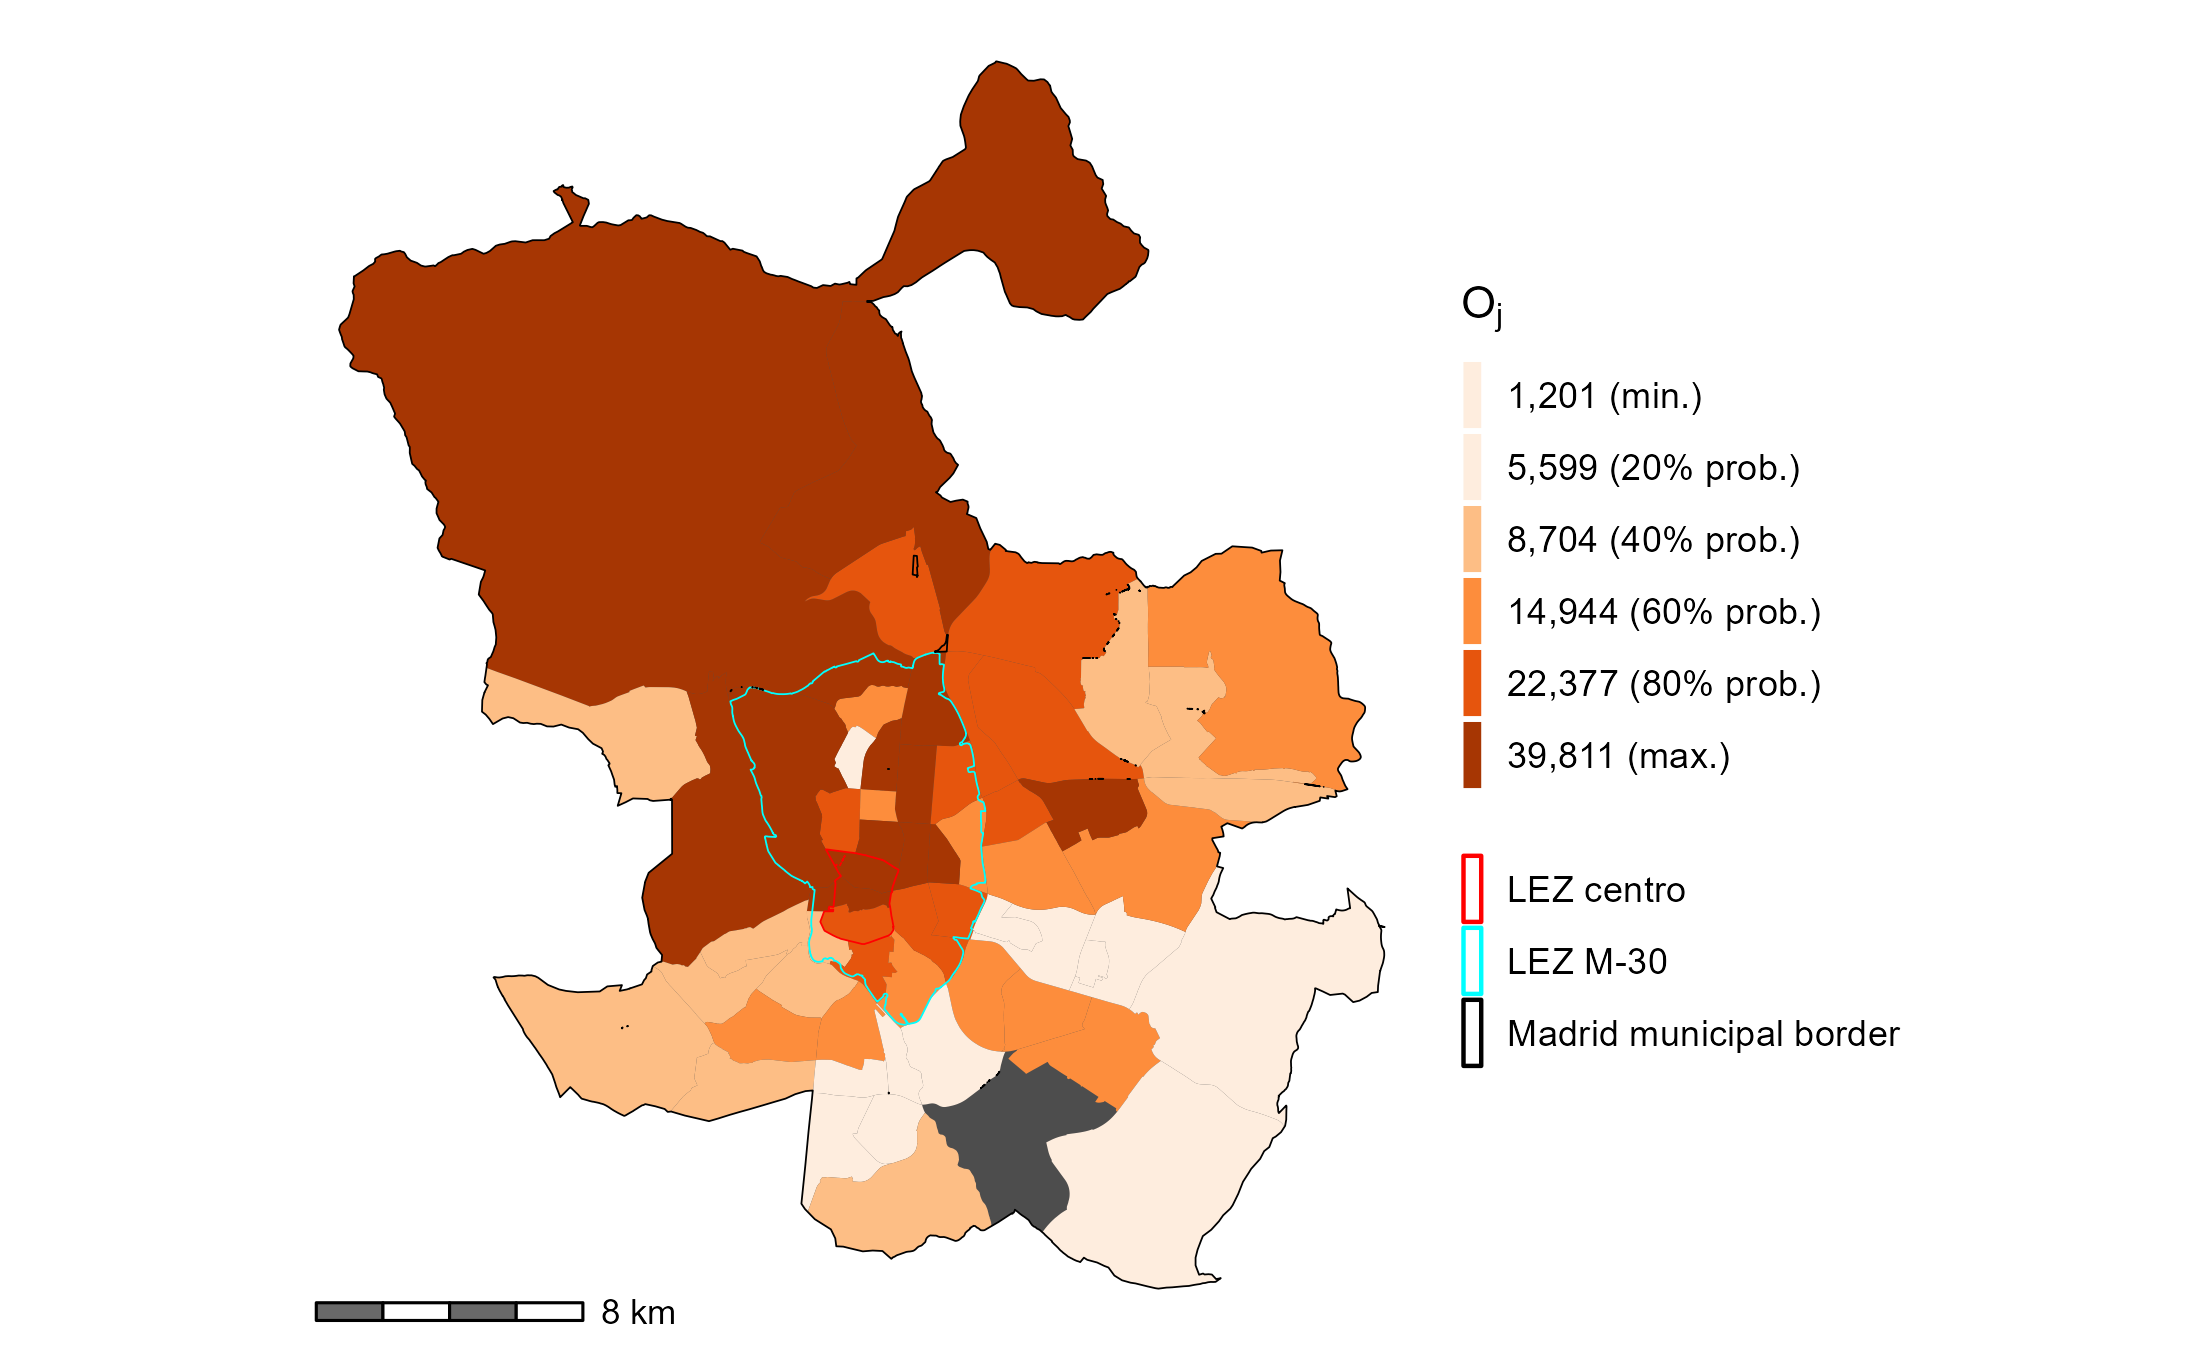
\includegraphics[width=1\linewidth]{images/i_jobs_zn208_plot} 
%DIFDELCMD < %%%
\DIFdelendFL \DIFaddbeginFL 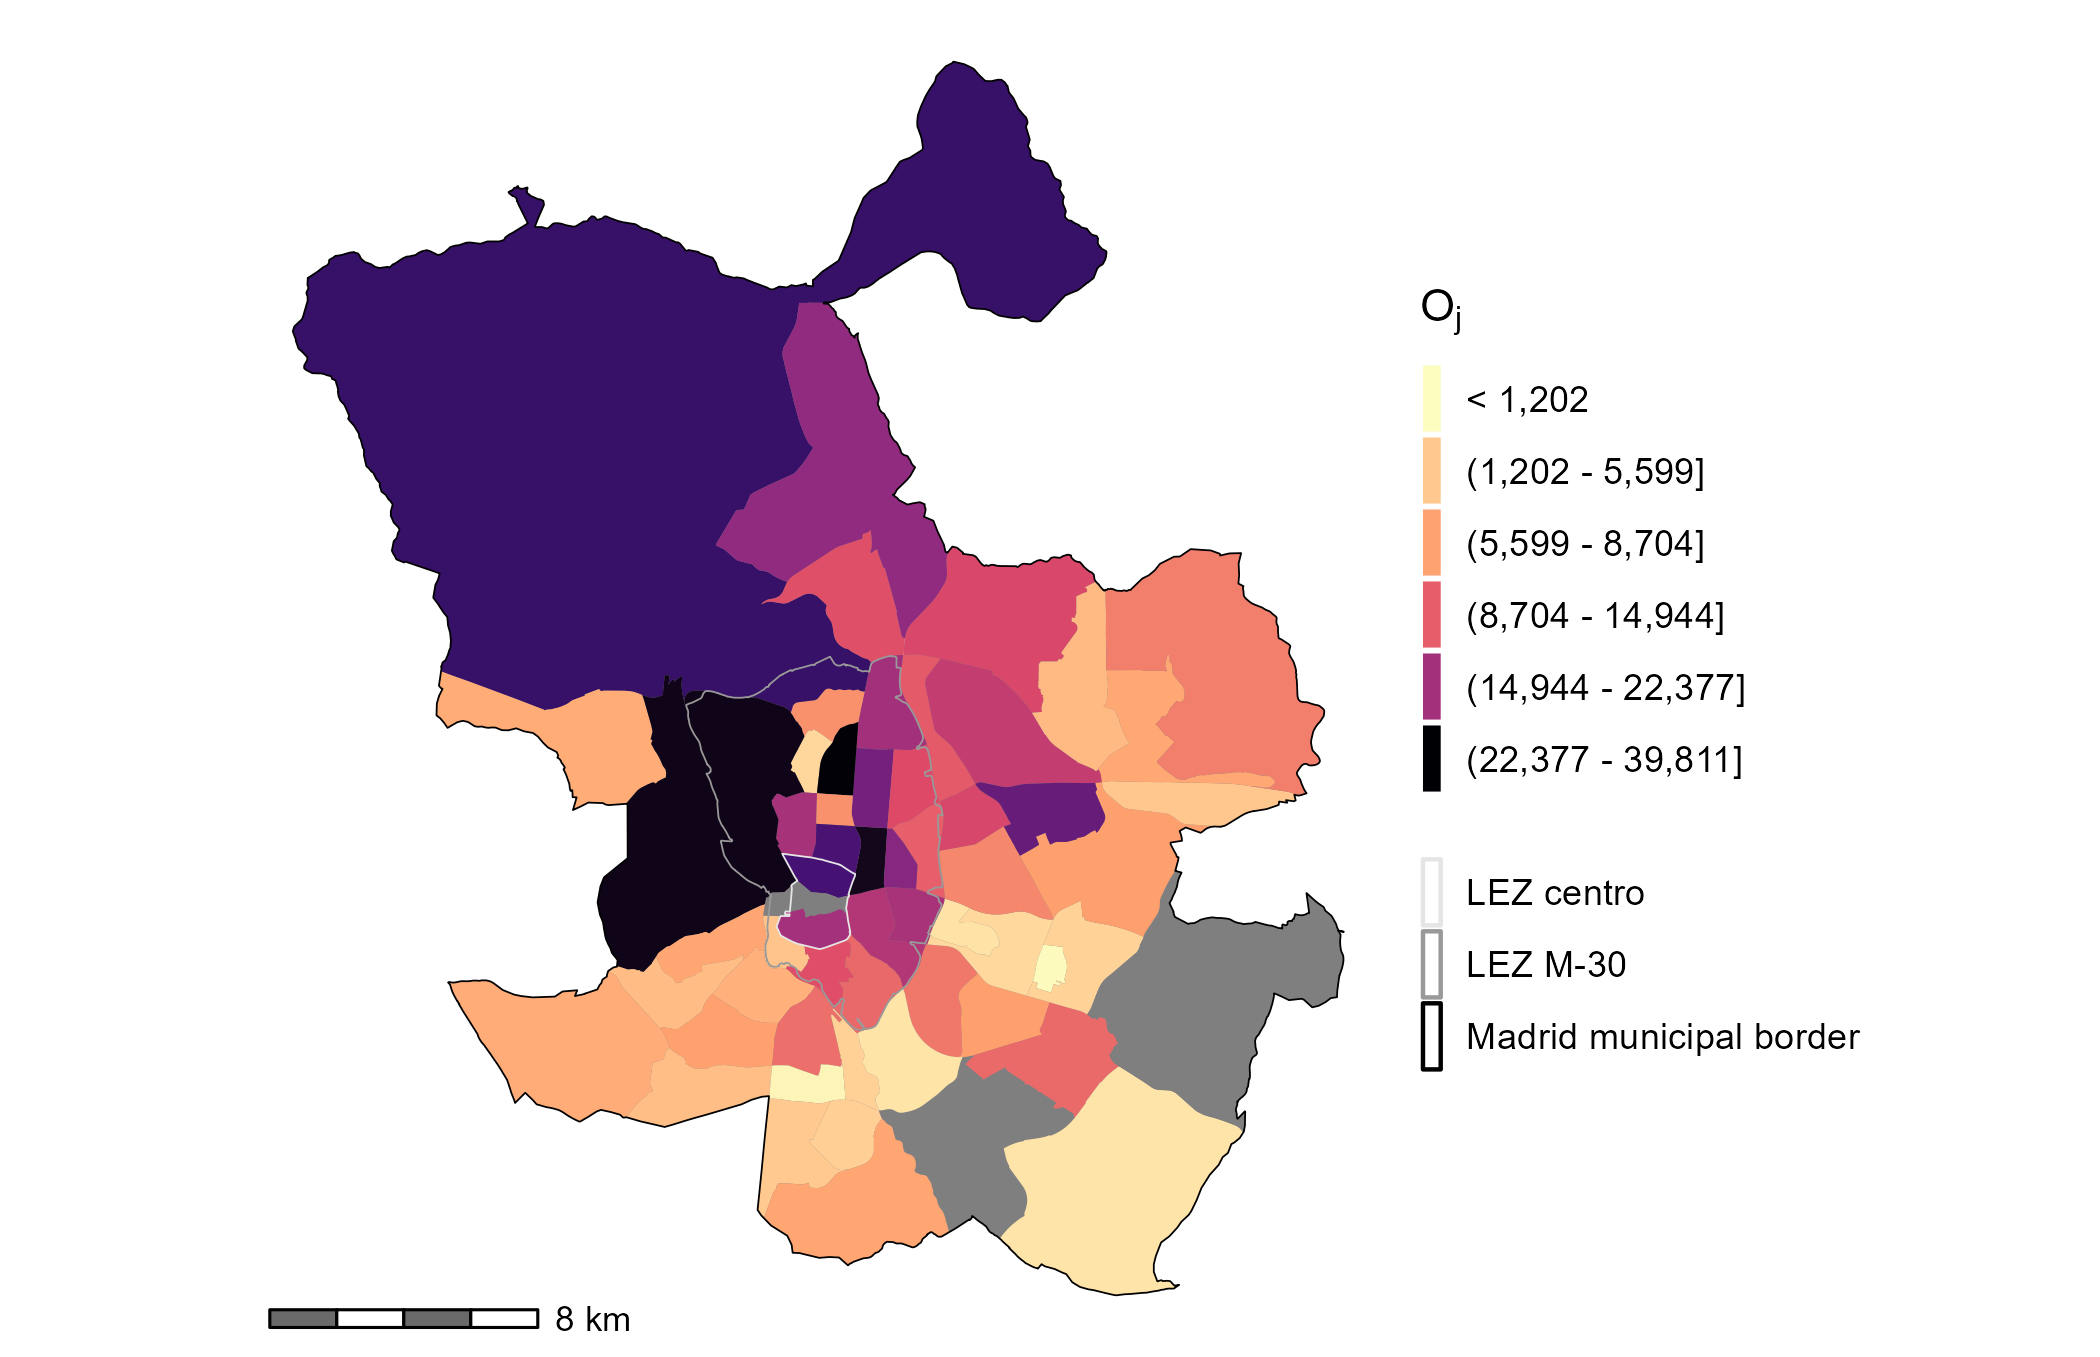
\includegraphics[width=0.85\linewidth]{images/Fig2} 
\DIFaddendFL 

}

\caption{\label{fig:Fig2} \DIFdelbeginFL \DIFdelFL{Jobs $O_j$ }\DIFdelendFL \DIFaddbeginFL \DIFaddFL{Distribution of jobs }\DIFaddendFL taken by people living and working in Madrid as reported \DIFdelbeginFL \DIFdelFL{by }\DIFdelendFL \DIFaddbeginFL \DIFaddFL{in }\DIFaddendFL the 2018 travel survey. \DIFaddbeginFL \DIFaddFL{Grey TAZs has no jobs. Ranges of values in the legend are quintiles.}\DIFaddendFL }\label{fig:jobs-plot}
\end{figure}

\begin{figure}

{\centering \DIFdelbeginFL %DIFDELCMD < 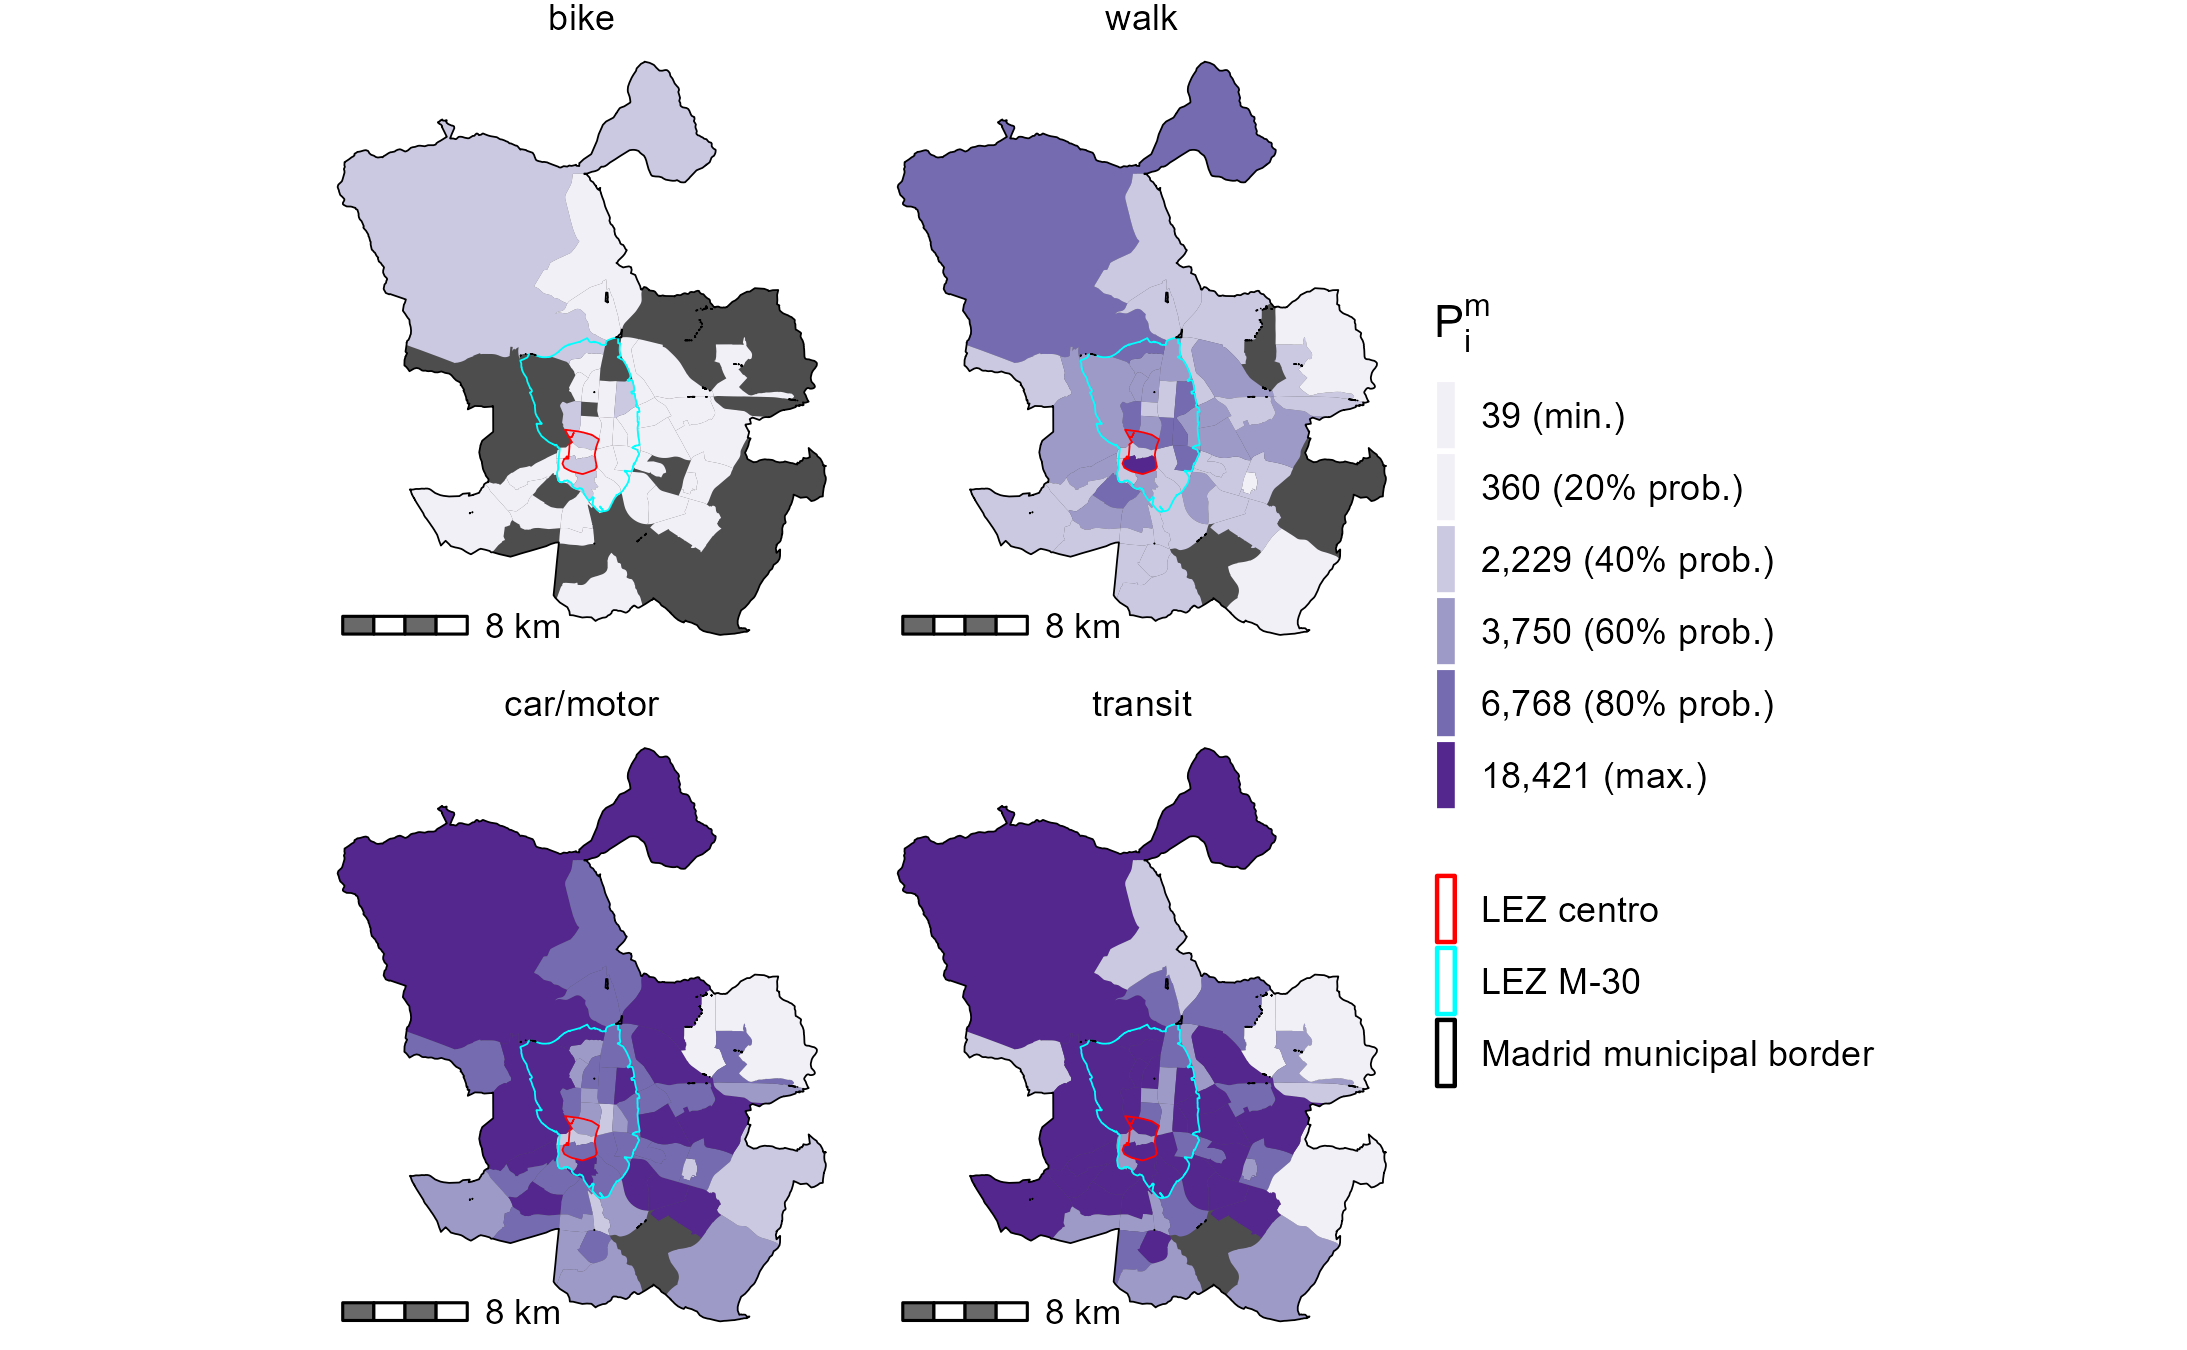
\includegraphics[width=1\linewidth]{images/im_populations_zn208_plot} 
%DIFDELCMD < %%%
\DIFdelendFL \DIFaddbeginFL 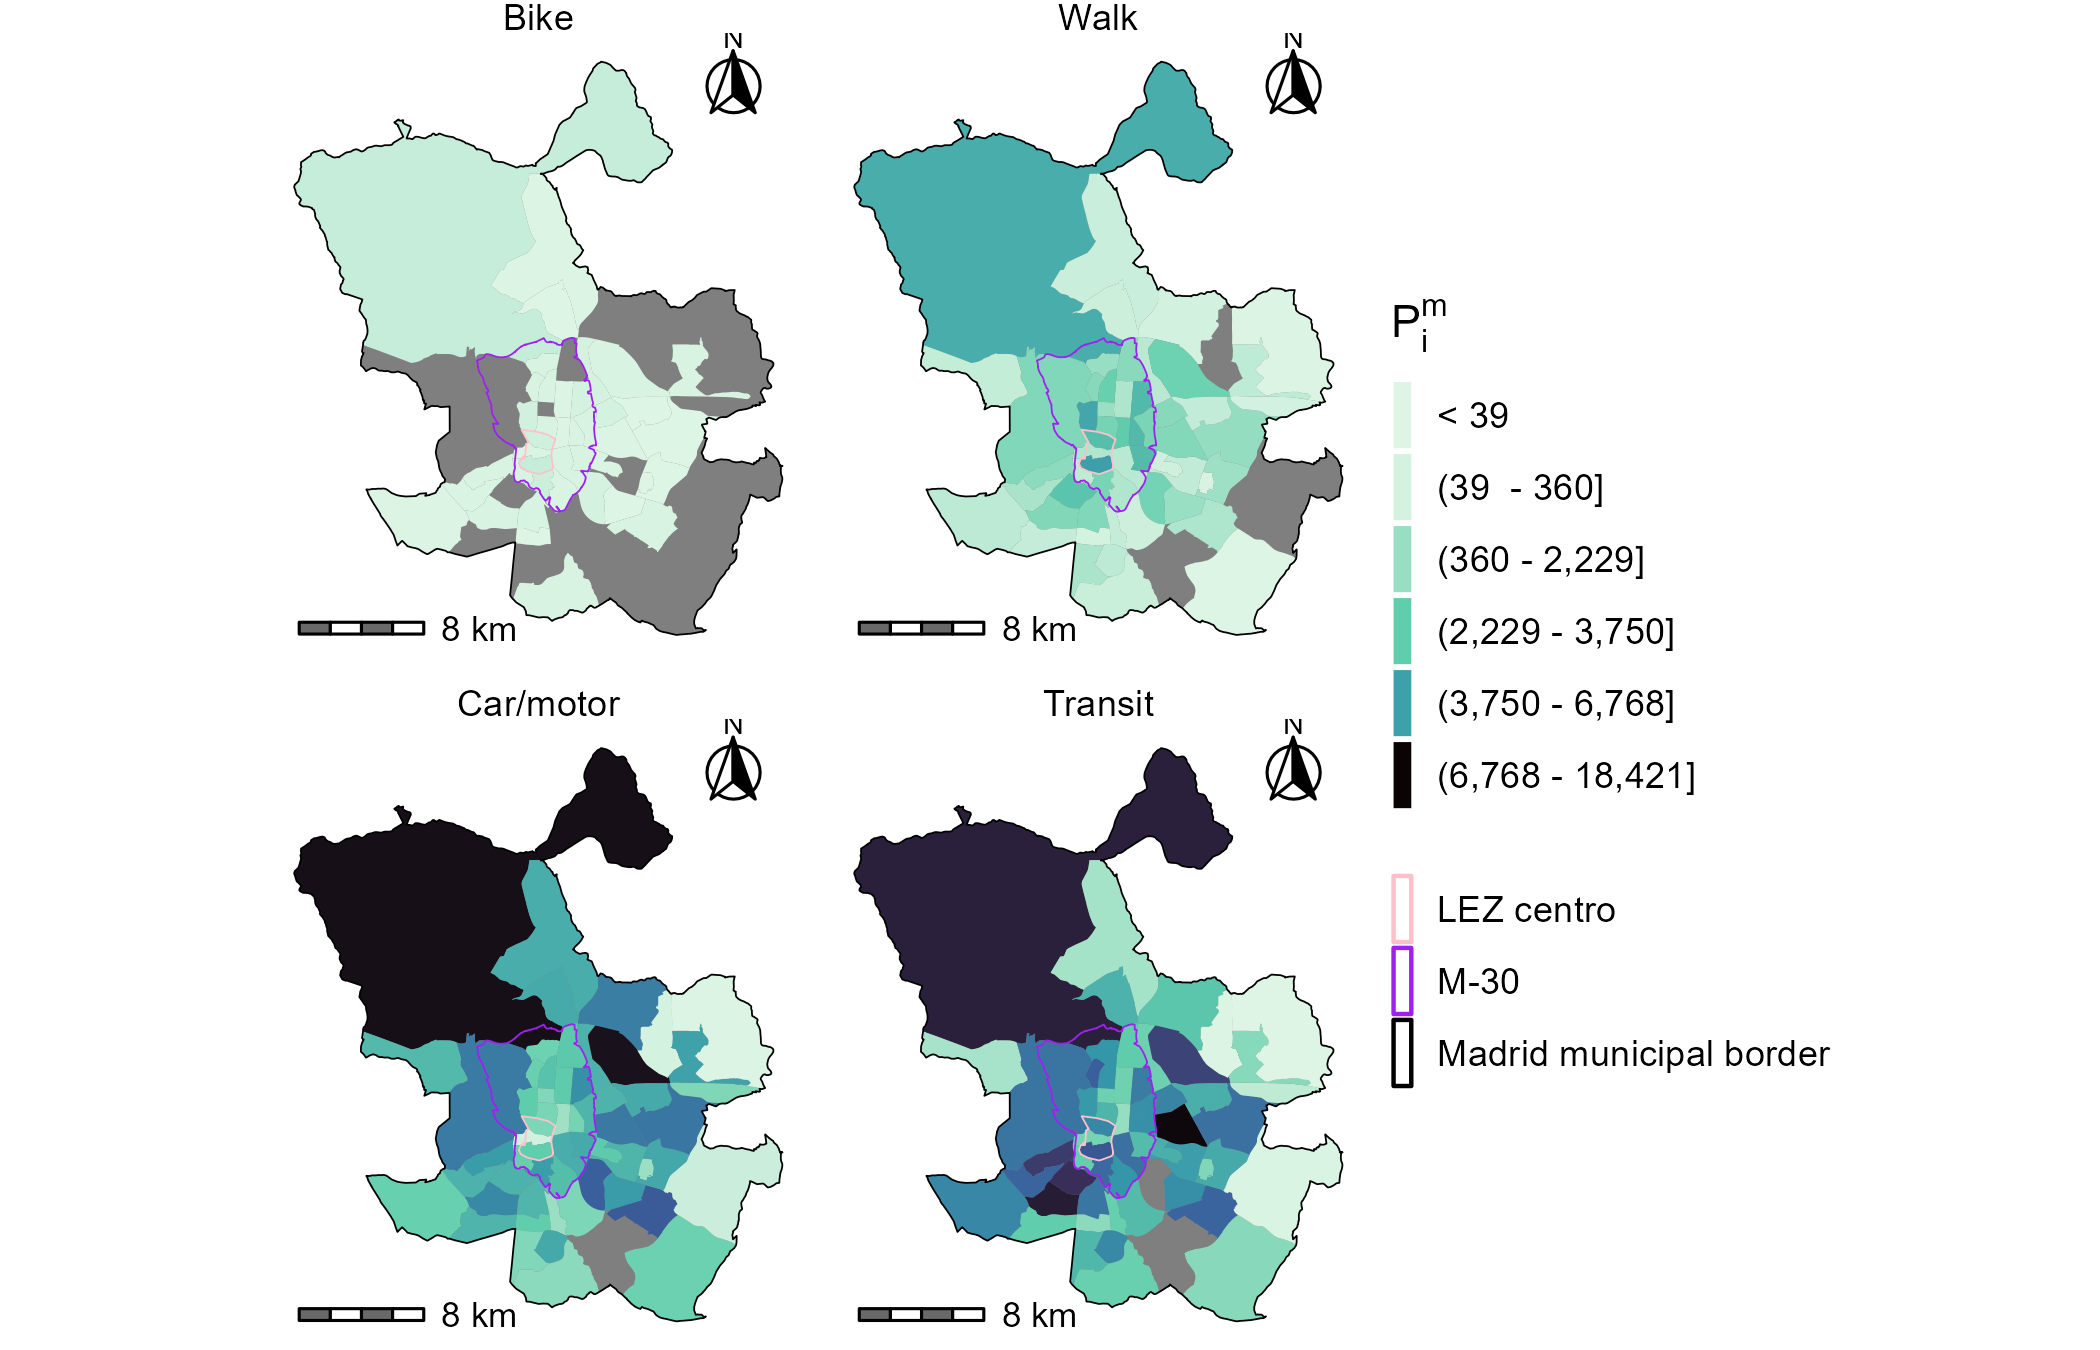
\includegraphics[width=0.85\linewidth]{images/Fig3} 
\DIFaddendFL 

}

\caption{\label{fig:Fig3} Population living and working in Madrid \DIFdelbeginFL \DIFdelFL{, }\DIFdelendFL by \DIFdelbeginFL \DIFdelFL{four summarized modal categories, $P^m_i$ }\DIFdelendFL \DIFaddbeginFL \DIFaddFL{mode of transportation }\DIFaddendFL as reported \DIFdelbeginFL \DIFdelFL{by }\DIFdelendFL \DIFaddbeginFL \DIFaddFL{in }\DIFaddendFL the 2018 travel survey. \DIFaddbeginFL \DIFaddFL{Grey TAZs have no population. Ranges of values in the legend are quintiles.}\DIFaddendFL }\label{fig:pop-plot}
\end{figure}

\DIFdelbegin \DIFdel{The }\DIFdelend \DIFaddbegin \hypertarget{data}{%
\subsection{Data}\label{data}}

\DIFadd{The source of data for our empirical example is the }\DIFaddend 2018 \DIFaddbegin \DIFadd{Travel Survey
of the }\DIFaddend Community of Madrid \DIFdelbegin \DIFdel{travel survey (}\DIFdelend {[}\DIFdelbegin \DIFdel{26}\DIFdelend \DIFaddbegin \DIFadd{42}\DIFaddend {]}\DIFdelbegin \DIFdel{) is the source of
data for this empirical example: it is }\DIFdelend \DIFaddbegin \DIFadd{. This is }\DIFaddend a representative survey
that \DIFdelbegin \DIFdel{reflects }\DIFdelend \DIFaddbegin \DIFadd{offers }\DIFaddend a snap-shot of \DIFdelbegin \DIFdel{the }\DIFdelend travel patterns for \DIFdelbegin \DIFdel{one typical day of the
working week (e.g., n=}\DIFdelend \DIFaddbegin \DIFadd{a typical weekday in
2018. The survey collected }\DIFaddend 222,744 trips \DIFdelbegin \DIFdel{with representative population
elevation factors) }\DIFdelend \DIFaddbegin \DIFadd{from a representative sample of
85,064 households across the traffic analysis zones (TAZ) in the
Community of Madrid. For context, the population older than 3 years in
the Community is 6,507,184.
}

\DIFadd{In this example, we use all home-to-full-time-work trips, by all modes}\DIFaddend .
\DIFdelbegin \DIFdel{In this paper, a sample of the travel survey is used,namely the residential home origin to work destination tripsof
all modesand those that originate and end in the city of Madrid.
These
totals are displayed in Figure \ref{fig:Fig2}
and Figure \ref{fig:Fig3} .
Both figures are displayed at the level of traffic analysis zones (\(i\)
and \(j\)) that correspond to the survey. The red }\DIFdelend \DIFaddbegin \DIFadd{The trips are expanded using population weights. Figures \ref{fig:Fig2}
and \ref{fig:Fig3} show the number of workers and the distribution of
full-time jobs in the City of Madrid by TAZ. The light grey }\DIFaddend boundary
represents the LEZ Centro in effect in \DIFdelbegin \DIFdel{2017 and thus those travel patterns of
car-restriction reflected in the survey . The cyan }\DIFdelend \DIFaddbegin \DIFadd{2017. The survey was conducted
after the introduction of LEZ Centro. The dark grey }\DIFaddend boundary represents
the LEZ \DIFdelbegin \DIFdel{that will be within }\DIFdelend \DIFaddbegin \DIFadd{planned for }\DIFaddend the boundaries of the M-30 highway \DIFdelbegin \DIFdel{in 2023
}\DIFdelend and is present in
the plots as a spatial reference for areas in proximity to the LEZ
Centro.

The total sum of jobs \(O_j\) \DIFdelbegin \DIFdel{that are held are }\DIFdelend \DIFaddbegin \DIFadd{are }\DIFaddend shown in Figure \ref{fig:Fig2} and the
populations that go to a work destination by four modal categories
\(P^m_i\), is \DIFdelbegin \DIFdel{reflected }\DIFdelend \DIFaddbegin \DIFadd{displayed }\DIFaddend in Figure \ref{fig:Fig3}. The modal \DIFdelbegin \DIFdel{categories represented }\DIFdelend \DIFaddbegin \DIFadd{shares }\DIFaddend in
Figure \ref{fig:Fig3} are \DIFdelbegin \DIFdel{summarized for
the
following trip mode types }\DIFdelend \DIFaddbegin \DIFadd{calculated based on those measured in the
survey. The modal categories and the mode types within each category are
reported as follows}\DIFaddend :

\begin{itemize}
\tightlist
\item
  Car/motor: all cars and operating modes (e.g., cab, private driver,
  company, rental \DIFdelbegin \DIFdel{care}\DIFdelend \DIFaddbegin \DIFadd{car}\DIFaddend , main driver \DIFdelbegin \DIFdel{, passenger, etc.}\DIFdelend \DIFaddbegin \DIFadd{of a private car, passenger in a
  private car}\DIFaddend ) and all public, private or company motorcycle/mopeds.
\item
  Transit: all bus, trams, and trains\DIFdelbegin \DIFdel{,
}\DIFdelend \DIFaddbegin \DIFadd{.
}\DIFaddend \item
  Bike: all bicycle trips (e.g., private, public, or company bike trips)
  and ``other'' types of micromobility options\DIFdelbegin \DIFdel{,
}\DIFdelend \DIFaddbegin \DIFadd{.
}\DIFaddend \item
  Walk: walking or by foot\DIFdelbegin \DIFdel{,
}\DIFdelend \DIFaddbegin \DIFadd{.
}\DIFaddend \end{itemize}

\DIFaddbegin \DIFadd{Some aggregation of modes is necessary to calculate the travel impedance
functions by mode. }\DIFaddend From Figure \ref{fig:Fig2}, it can be seen that the
largest concentration of jobs \DIFdelbegin \DIFdel{are }\DIFdelend \DIFaddbegin \DIFadd{is }\DIFaddend within, near, and to the north of \DIFdelbegin \DIFdel{the }\DIFdelend LEZ
Centro. The \DIFdelbegin \DIFdel{population that is accessing }\DIFdelend \DIFaddbegin \DIFadd{populations with access to }\DIFaddend those jobs by mode (Figure
\ref{fig:Fig3}) \DIFdelbegin \DIFdel{, appear }\DIFdelend \DIFaddbegin \DIFadd{are }\DIFaddend spatially distinct. \DIFdelbegin \DIFdel{Car and transit
trips
}\DIFdelend \DIFaddbegin \DIFadd{Travel by car and transit
}\DIFaddend represent 37\% and 47\% of the modal share respectively. The population
that travels \DIFdelbegin \DIFdel{using }\DIFdelend \DIFaddbegin \DIFadd{by }\DIFaddend transit is more spatially distributed than those using
cars - particularly near and within LEZ Centro. This distribution \DIFdelbegin \DIFdel{could be a result of a }\DIFdelend \DIFaddbegin \DIFadd{is
likely caused by a }\DIFaddend variety of factors including: transit coverage and
service within with city, effective car infrastructure outside of the
M-30, and/or the impact of the \DIFdelbegin \DIFdel{Central LEZ itself.
}%DIFDELCMD < 

%DIFDELCMD < %%%
\DIFdelend \DIFaddbegin \DIFadd{LEZ Centro itself. }\DIFaddend From Figure
\ref{fig:Fig3}, it can \DIFdelbegin \DIFdel{also }\DIFdelend be seen that \DIFdelbegin \DIFdel{biking and walking
trips are }\DIFdelend \DIFaddbegin \DIFadd{active travel is }\DIFaddend less common than
motorized trips at 1\% and 15\% \DIFdelbegin \DIFdel{respectively.
Noteably}\DIFdelend \DIFaddbegin \DIFadd{for cycling and walking respectively.
Noticeably}\DIFaddend , there is a positive trend between the \DIFdelbegin \DIFdel{populations of walking and biking trips in
zones and populations of transit trips}\DIFdelend \DIFaddbegin \DIFadd{walking and cycling in
zones where transit is also present}\DIFaddend . This positive trend is higher than
for car trip populations.

\DIFdelbegin \DIFdel{The travel time for each trip is }\DIFdelend \DIFaddbegin \DIFadd{Travel times are }\DIFaddend provided within the \DIFdelbegin \DIFdel{survey. These
travel times, per modal category, are }\DIFdelend \DIFaddbegin \DIFadd{travel survey by mode. This
information is }\DIFaddend used to calibrate mode-specific travel impedance
functions \(f^m(c_{ij}^m)\). To illustrate the modal differences in
travel \DIFdelbegin \DIFdel{lengths, summary descriptive }\DIFdelend \DIFaddbegin \DIFadd{times, the following descriptive statistics }\DIFaddend per mode are
\DIFdelbegin \DIFdel{detailed}\DIFdelend \DIFaddbegin \DIFadd{presented}\DIFaddend :

\begin{itemize}
\tightlist
\item
  Car/motor: \DIFaddbegin \DIFadd{mean }\DIFaddend 36 \DIFdelbegin \DIFdel{min }\DIFdelend \DIFaddbegin \DIFadd{minutes }\DIFaddend (min: 0 \DIFdelbegin \DIFdel{min.}\DIFdelend \DIFaddbegin \DIFadd{minutes}\DIFaddend , Q2: 15 \DIFdelbegin \DIFdel{min.}\DIFdelend \DIFaddbegin \DIFadd{minutes}\DIFaddend , Q3: 55
  \DIFdelbegin \DIFdel{min.}\DIFdelend \DIFaddbegin \DIFadd{minutes}\DIFaddend , max: 120 \DIFdelbegin \DIFdel{min.}\DIFdelend \DIFaddbegin \DIFadd{minutes}\DIFaddend )
\item
  Transit: \DIFaddbegin \DIFadd{mean }\DIFaddend 55 \DIFdelbegin \DIFdel{min. }\DIFdelend \DIFaddbegin \DIFadd{minutes }\DIFaddend (min: 1 \DIFdelbegin \DIFdel{min.}\DIFdelend \DIFaddbegin \DIFadd{minutes}\DIFaddend , Q2: 30 \DIFdelbegin \DIFdel{min.}\DIFdelend \DIFaddbegin \DIFadd{minutes}\DIFaddend , Q3: 80
  \DIFdelbegin \DIFdel{min.}\DIFdelend \DIFaddbegin \DIFadd{minutes}\DIFaddend , max: 120 \DIFdelbegin \DIFdel{min.}\DIFdelend \DIFaddbegin \DIFadd{minutes}\DIFaddend )
\item
  Bike: \DIFaddbegin \DIFadd{mean }\DIFaddend 34 \DIFdelbegin \DIFdel{min. }\DIFdelend \DIFaddbegin \DIFadd{minutes }\DIFaddend (min: 5 \DIFdelbegin \DIFdel{min.}\DIFdelend \DIFaddbegin \DIFadd{minutes}\DIFaddend , Q2: 15 \DIFdelbegin \DIFdel{min.}\DIFdelend \DIFaddbegin \DIFadd{minutes}\DIFaddend , Q3: 40 \DIFdelbegin \DIFdel{min.}\DIFdelend \DIFaddbegin \DIFadd{minutes}\DIFaddend ,
  max: 115 \DIFdelbegin \DIFdel{min.}\DIFdelend \DIFaddbegin \DIFadd{minutes}\DIFaddend )
\item
  Walk: \DIFaddbegin \DIFadd{mean }\DIFaddend 27 \DIFdelbegin \DIFdel{min. }\DIFdelend \DIFaddbegin \DIFadd{minutes }\DIFaddend (min: 1 \DIFdelbegin \DIFdel{min.}\DIFdelend \DIFaddbegin \DIFadd{minutes}\DIFaddend , Q2: 10 \DIFdelbegin \DIFdel{min.}\DIFdelend \DIFaddbegin \DIFadd{minutes}\DIFaddend , Q3: 45 \DIFdelbegin \DIFdel{min.}\DIFdelend \DIFaddbegin \DIFadd{minutes}\DIFaddend ,
  max: 119 \DIFdelbegin \DIFdel{min.}\DIFdelend \DIFaddbegin \DIFadd{minutes}\DIFaddend )
\end{itemize}

\DIFdelbegin \DIFdel{To calculate }\DIFdelend \DIFaddbegin \DIFadd{Impedance functions }\DIFaddend \(f^m(c_{ij}^m)\) \DIFdelbegin \DIFdel{from the survey travel
times , a concept
known as the }\DIFdelend \DIFaddbegin \DIFadd{are calibrated from the travel
times in the survey via the empirical }\DIFaddend trip length distribution (TLD)\DIFdelbegin \DIFdel{was used. A TLD represents
}\DIFdelend \DIFaddbegin \DIFadd{. An
empirical TLD is given by }\DIFaddend the proportion of trips \DIFdelbegin \DIFdel{that are taken at a specific travel cost
such as
travel time (i.e., probability density distribution of trips taken by
travel cost)}\DIFdelend \DIFaddbegin \DIFadd{at various travel cost
bins}\DIFaddend . This distribution is then used to \DIFdelbegin \DIFdel{derive impedance
functions (e.g., done in the accessibility works of }\DIFdelend \DIFaddbegin \DIFadd{estimate the parameters of a
function for the travel impedance }\DIFaddend {[}\DIFdelbegin \DIFdel{27}\DIFdelend \DIFaddbegin \DIFadd{as done in 43,44,45}\DIFaddend {]\DIFdelbegin %DIFDELCMD < }%%%
\DIFdel{,}%DIFDELCMD < {[%%%
\DIFdelend }\DIFdelbegin \DIFdel{28}%DIFDELCMD < {]}%%%
\DIFdel{,and }%DIFDELCMD < {[}%%%
\DIFdel{29}%DIFDELCMD < {]}%%%
\DIFdel{). }\DIFdelend \DIFaddbegin \DIFadd{. To fit the
impedance functions, we use the }\DIFaddend Maximum likelihood estimation and the
Nelder-Mead method for direct optimization available within the R
\{fitdistrplus\} package {[}\DIFdelbegin \DIFdel{30}\DIFdelend \DIFaddbegin \DIFadd{46}\DIFaddend {]}\DIFdelbegin \DIFdel{is used to fit the impedance functions. As shown as shown in
Figure \ref{fig:Fig4}, based }\DIFdelend \DIFaddbegin \DIFadd{. Based }\DIFaddend on goodness-of-fit criteria and
associated diagnostics, the gamma and log-normal probability density
\DIFdelbegin \DIFdel{function (line
curves) }\DIFdelend \DIFaddbegin \DIFadd{functions }\DIFaddend are selected as best fitting curves for the motorized and
non-motorized modes respectively. The selection of functional \DIFdelbegin \DIFdel{form
}\DIFdelend \DIFaddbegin \DIFadd{forms
}\DIFaddend aligns with empirical examples in other regions {[}\DIFdelbegin \DIFdel{14,31,32}\DIFdelend \DIFaddbegin \DIFadd{15,47,48}\DIFaddend {]}. \DIFdelbegin \DIFdel{Overall, the plots in Figure \ref{fig:Fig4} display the probability of travel }\DIFdelend \DIFaddbegin \DIFadd{The
shape and rate parameters for the gamma functions (motorized modes) are
1.8651852 and 0.051468 for car/motor and 2.7566235 and 0.0499193 for
transit; for the log-normal functions (non-motorized modes), the mean
and standard deviation parameters are 3.2372212 and 0.7575986 for bike
and 2.9918042 and 0.7575986 for walk.
}

\DIFadd{Figure \ref{fig:Fig4} includes four plots to visualize the calibrated
impedance functions (represented as black lines) superimposed on the
empirical TLD. The impedance functions can be interpreted as the
propensity to travel (y-axis) }\DIFaddend given a trip travel time \DIFdelbegin \DIFdel{, based on trip flows from the survey. These
`probability of travel' at each travel time for each mode are realized
observations that reflect the land-use, }\DIFdelend \DIFaddbegin \DIFadd{(x-axis). The
functions reflect a combination of possibilities and preferences: the
travel behavior given the transportation technologies available. For
example, trips shorter than 5 minutes do not occur frequently for any
mode; this reflects the spatial separation between places of residence
and places of work commonly seen in many cities. In terms of }\DIFaddend the
\DIFdelbegin \DIFdel{transport system, and }\DIFdelend \DIFaddbegin \DIFadd{non-motorized modes, there is a preference towards walking trips around
15 minutes in duration, as seen from the highest value of
\(f^{walk}(c_{ij}^{walk})\). With respect to travel by bicycle, longer
travel times are more common; although the highest value of the
impedance also corresponds to approximately 15 minutes, the curve has a
longer tail and values decrease less rapidly at longer travel times than
is the case of \(f^{walk}(c_{ij}^{walk})\). A similar trend can be
observed for }\DIFaddend the \DIFdelbegin \DIFdel{population travel behaviour in Madrid}\DIFdelend \DIFaddbegin \DIFadd{motorized modal options where transit mode is more
spread out than car/motor mode. All in all, these functions represent
the propensity of travel by mode by duration of trip, and are used to
calculate the proportional allocation factors \(F_{ij}^m\) for
\(V_i^m\)}\DIFaddend .

\begin{figure}

{\centering \DIFdelbeginFL %DIFDELCMD < 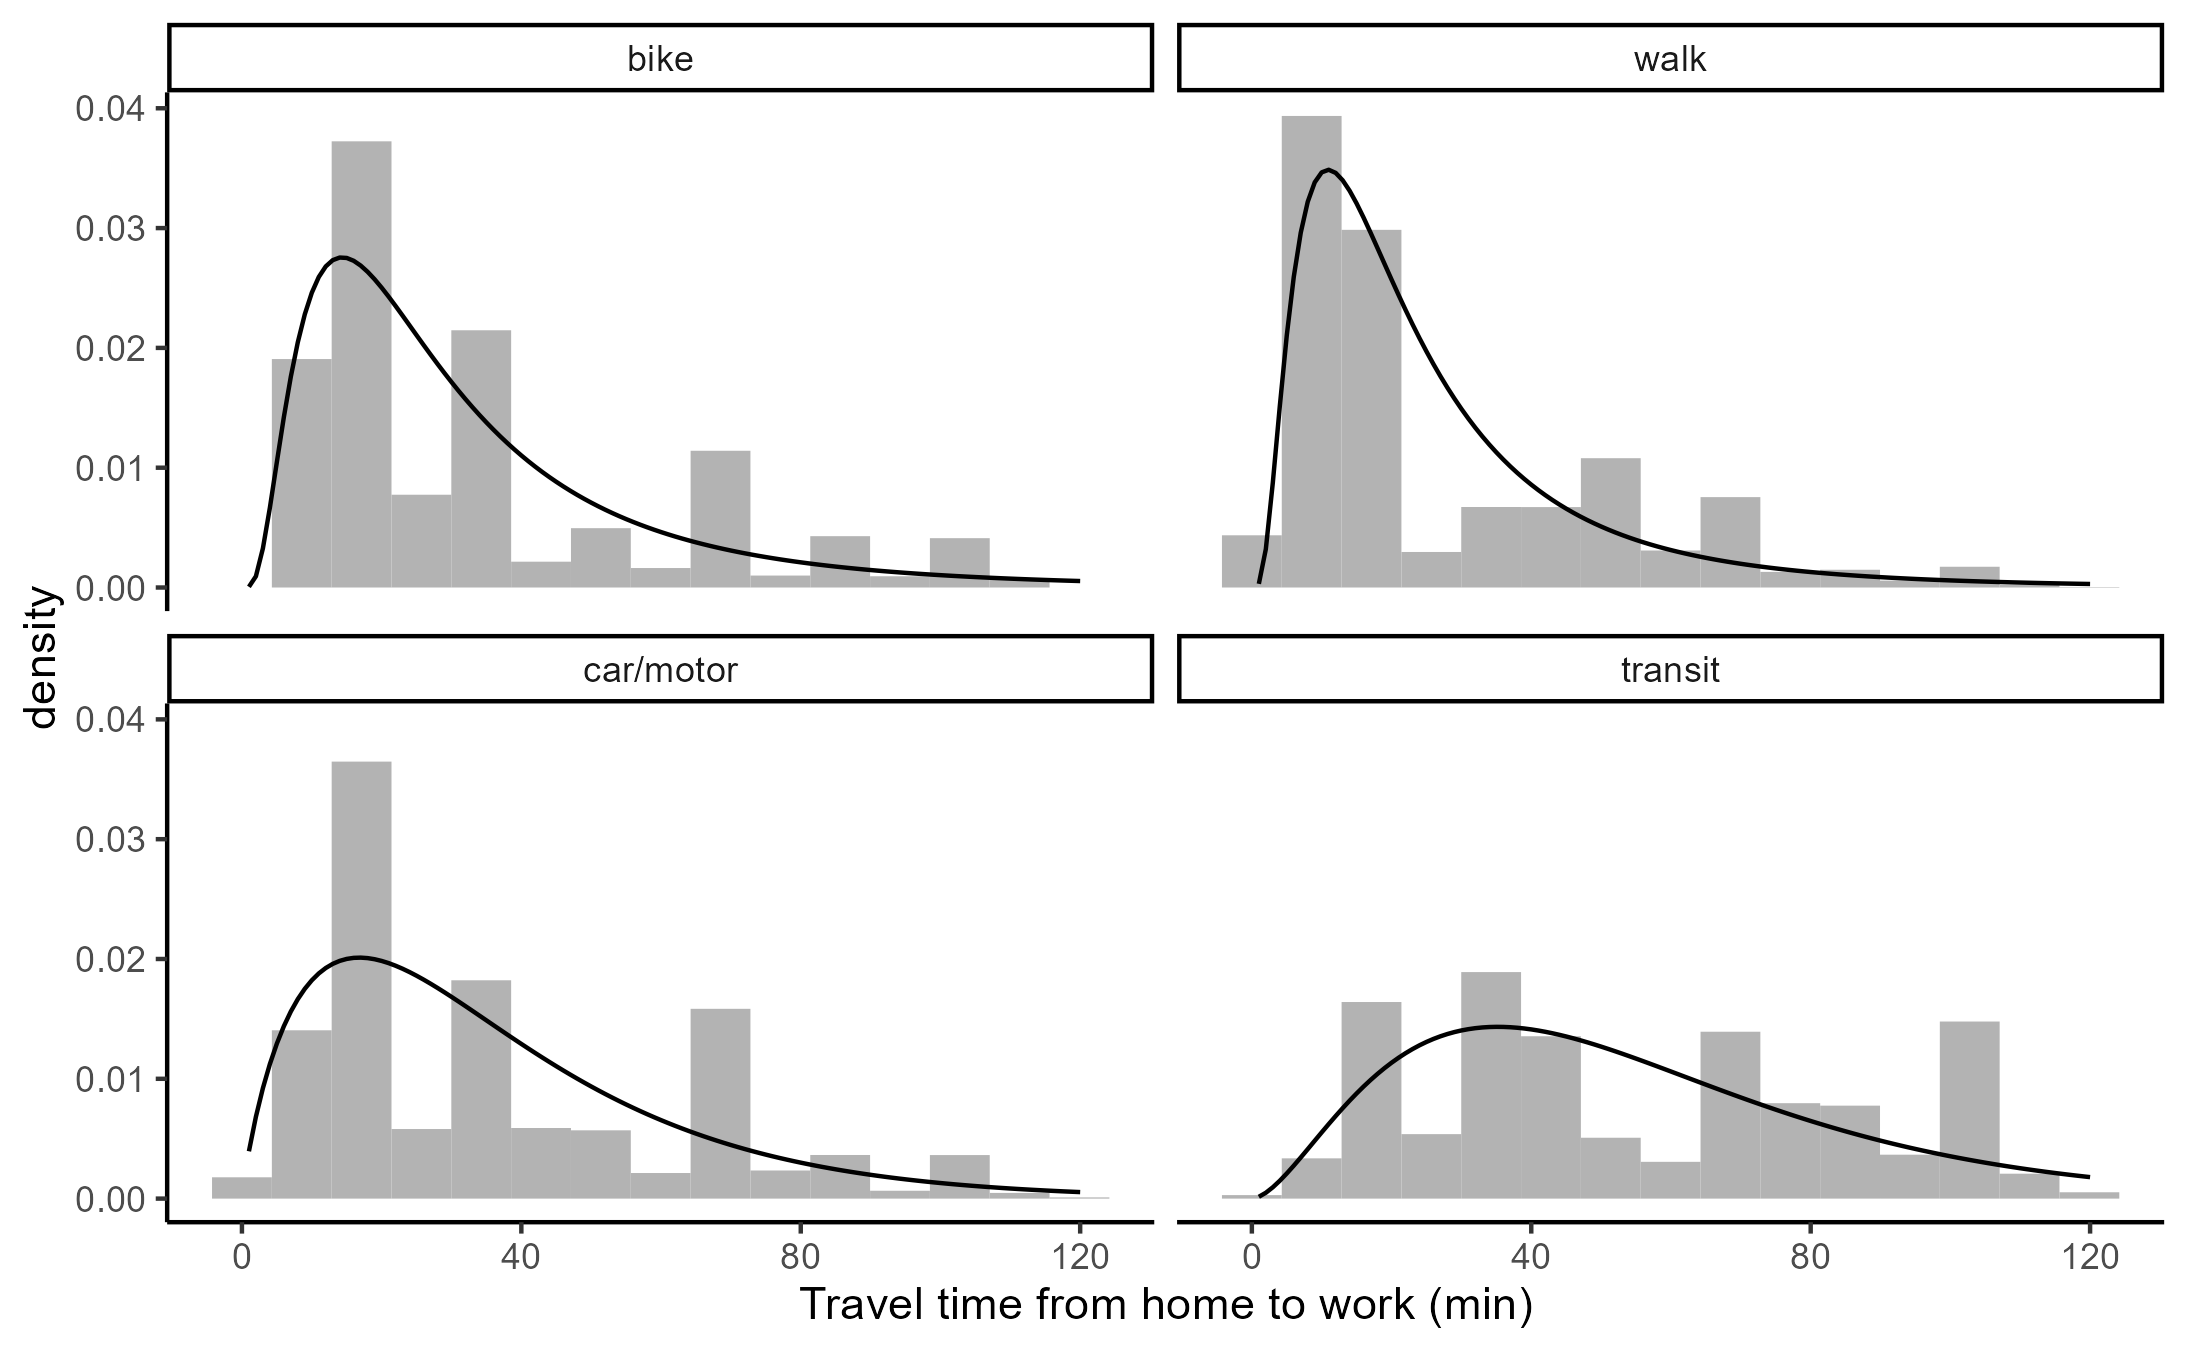
\includegraphics[width=1\linewidth]{images/tlds_curves_m_plot} 
%DIFDELCMD < %%%
\DIFdelendFL \DIFaddbeginFL 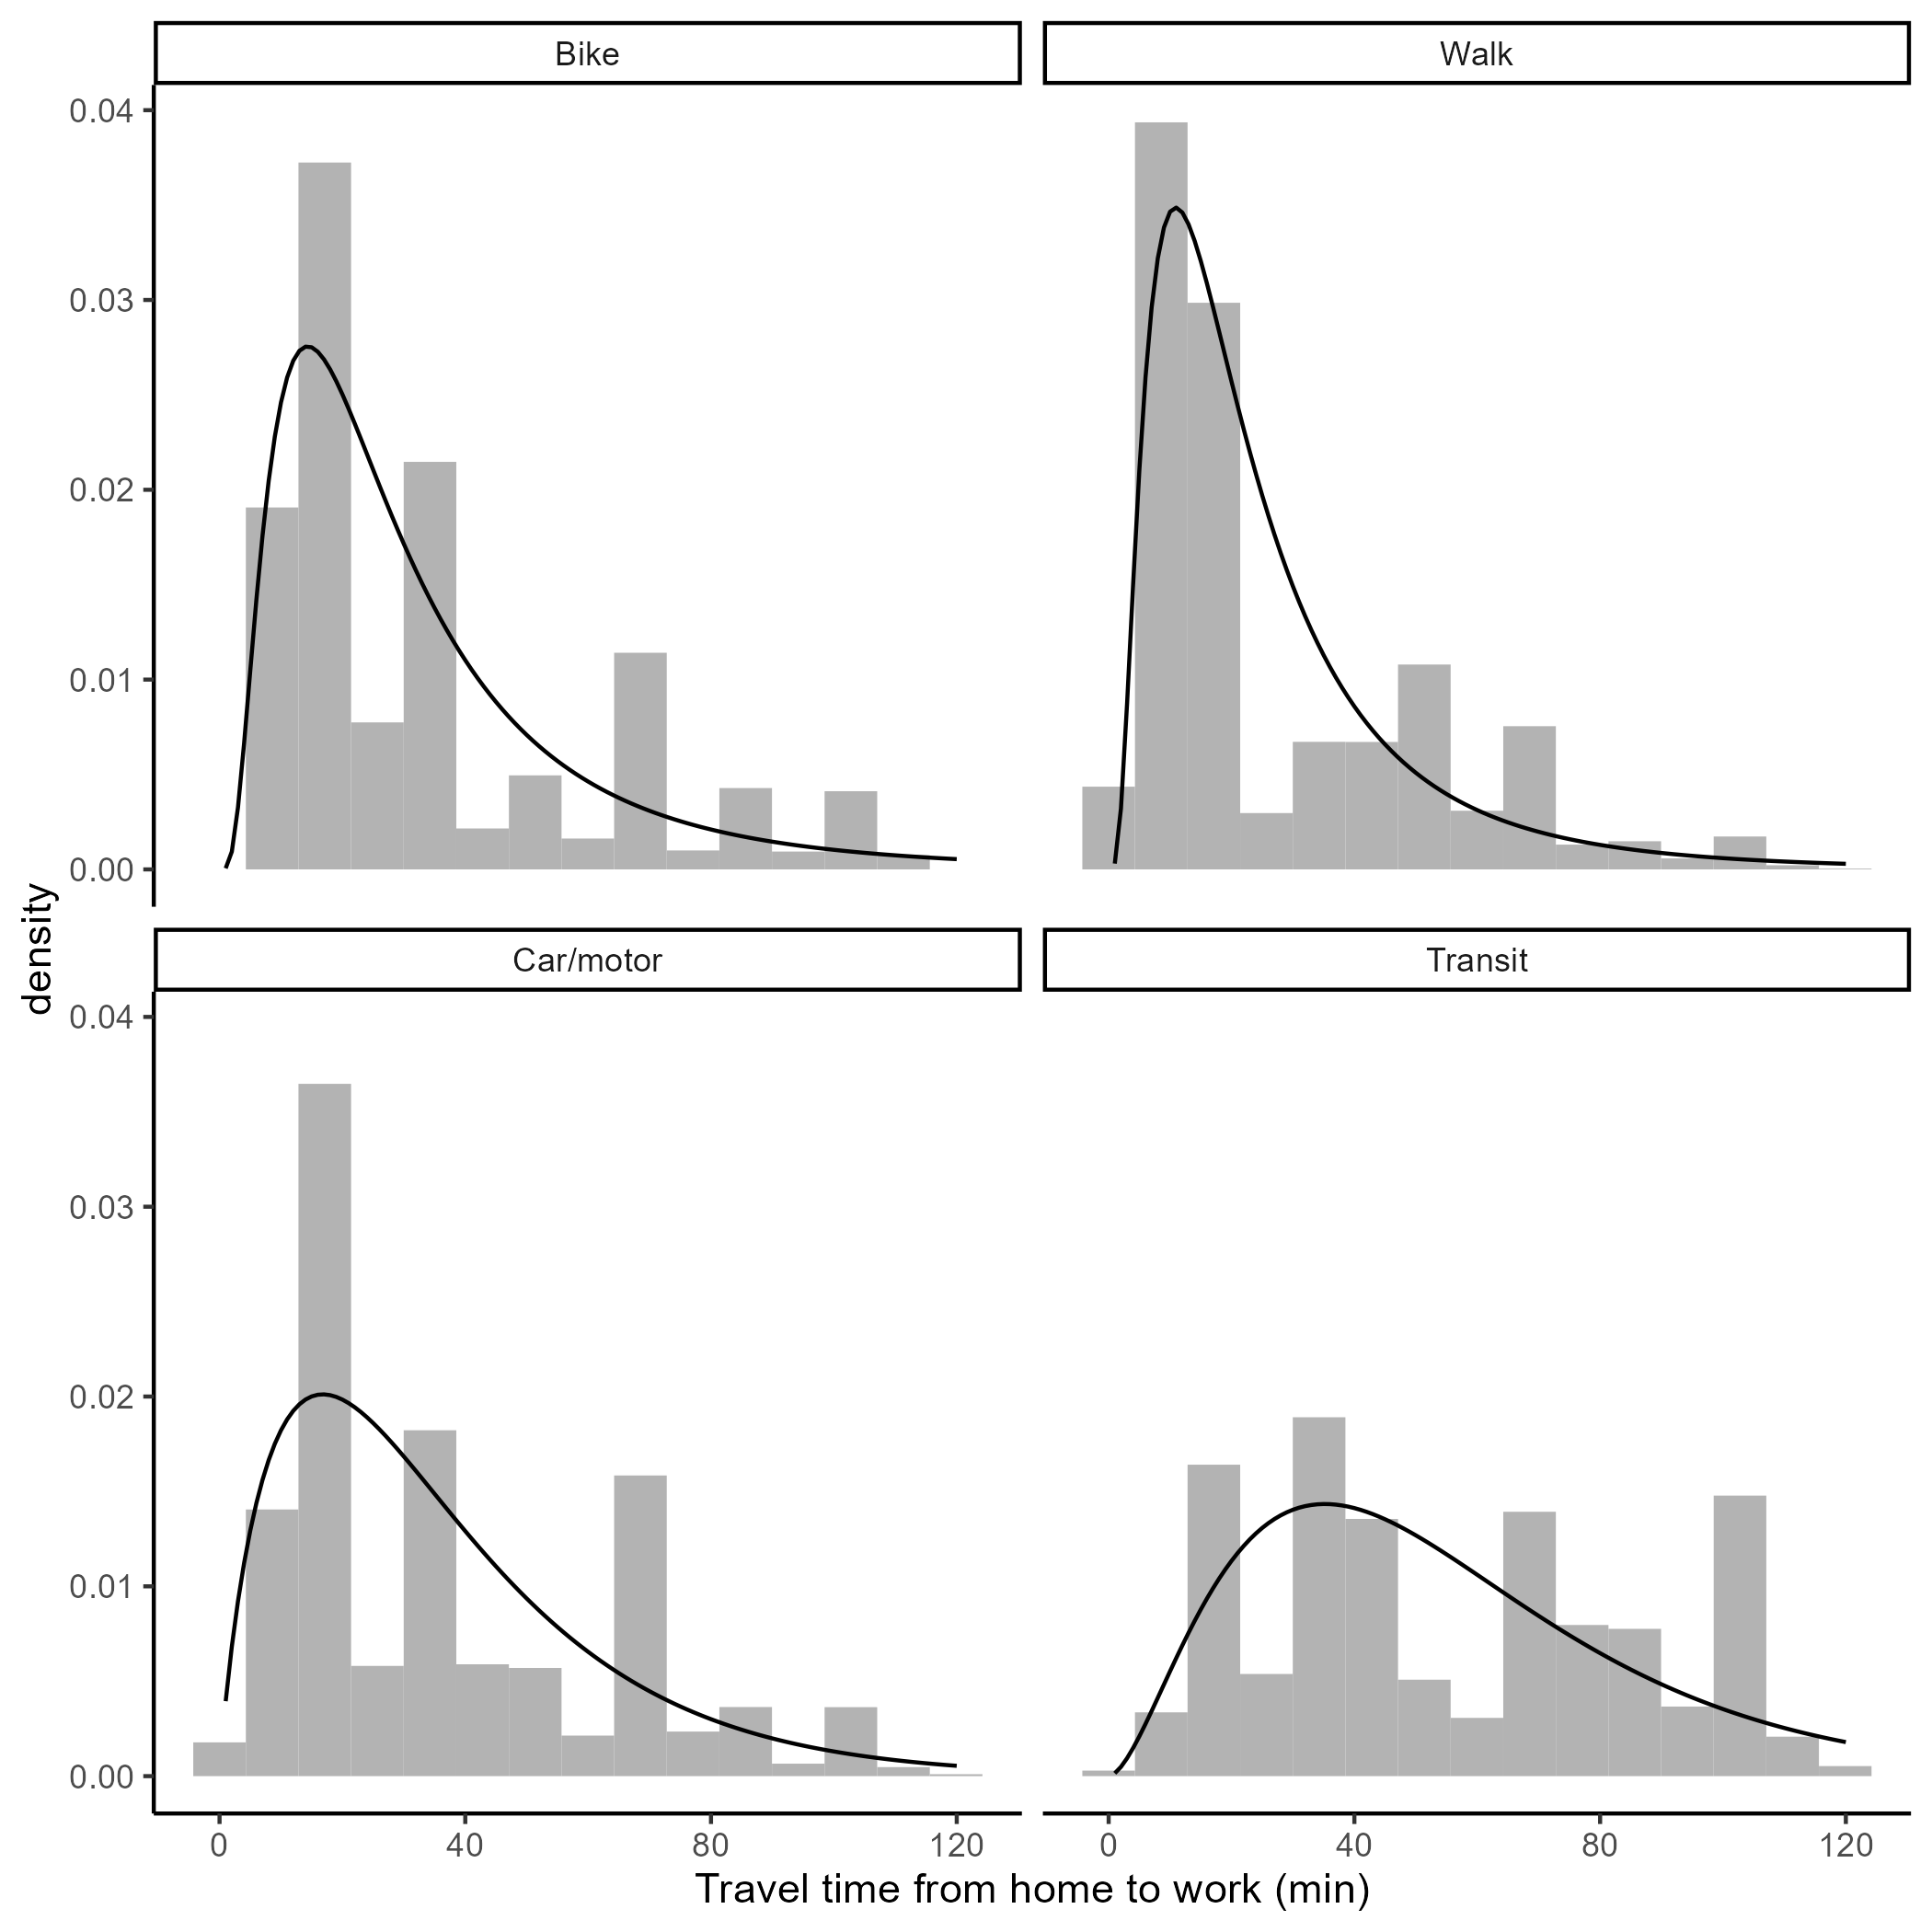
\includegraphics[width=0.85\linewidth]{images/Fig4} 
\DIFaddendFL 

}

\caption{\label{fig:Fig4} Fitted impedance function \DIFdelbeginFL \DIFdelFL{curve (line) }\DIFdelendFL against empirical TLD (bars) corresponding to the \DIFdelbeginFL \DIFdelFL{home-to-work origin-destination }\DIFdelendFL \DIFaddbeginFL \DIFaddFL{home to full-time work origin destination }\DIFaddendFL flows \DIFdelbeginFL \DIFdelFL{from }\DIFdelendFL \DIFaddbeginFL \DIFaddFL{for }\DIFaddendFL the \DIFaddbeginFL \DIFaddFL{City of }\DIFaddendFL Madrid \DIFaddbeginFL \DIFaddFL{from the }\DIFaddendFL 2018 travel survey.}\label{fig:tlds-curves-m-plot}
\end{figure}

\hypertarget{results}{%
\subsection{Results}\label{results}}

\DIFaddbegin \DIFadd{At this point, it is worthwhile reiterating that the empirical example
is a snap-shot of spatial availability by mode using data from the 2018
travel survey. Our purpose in this empirical example is to investigate
the trends in availability of employment opportunities by mode, and
illustrate how spatial availability can be used in discussions about the
competitive advantage of various modes within Madrid Centro. }\DIFaddend The spatial
availability of jobs \(V_i^m\) is calculated for each of the four \DIFdelbegin \DIFdel{modal categories }\DIFdelend \DIFaddbegin \DIFadd{modes
}\DIFaddend \(m\) at the level of traffic analysis zones \(i\) in Madrid and
\DIFdelbegin \DIFdel{demonstrated }\DIFdelend \DIFaddbegin \DIFadd{displayed }\DIFaddend in Figure \ref{fig:Fig5}.

\begin{figure}

{\centering \DIFdelbeginFL %DIFDELCMD < 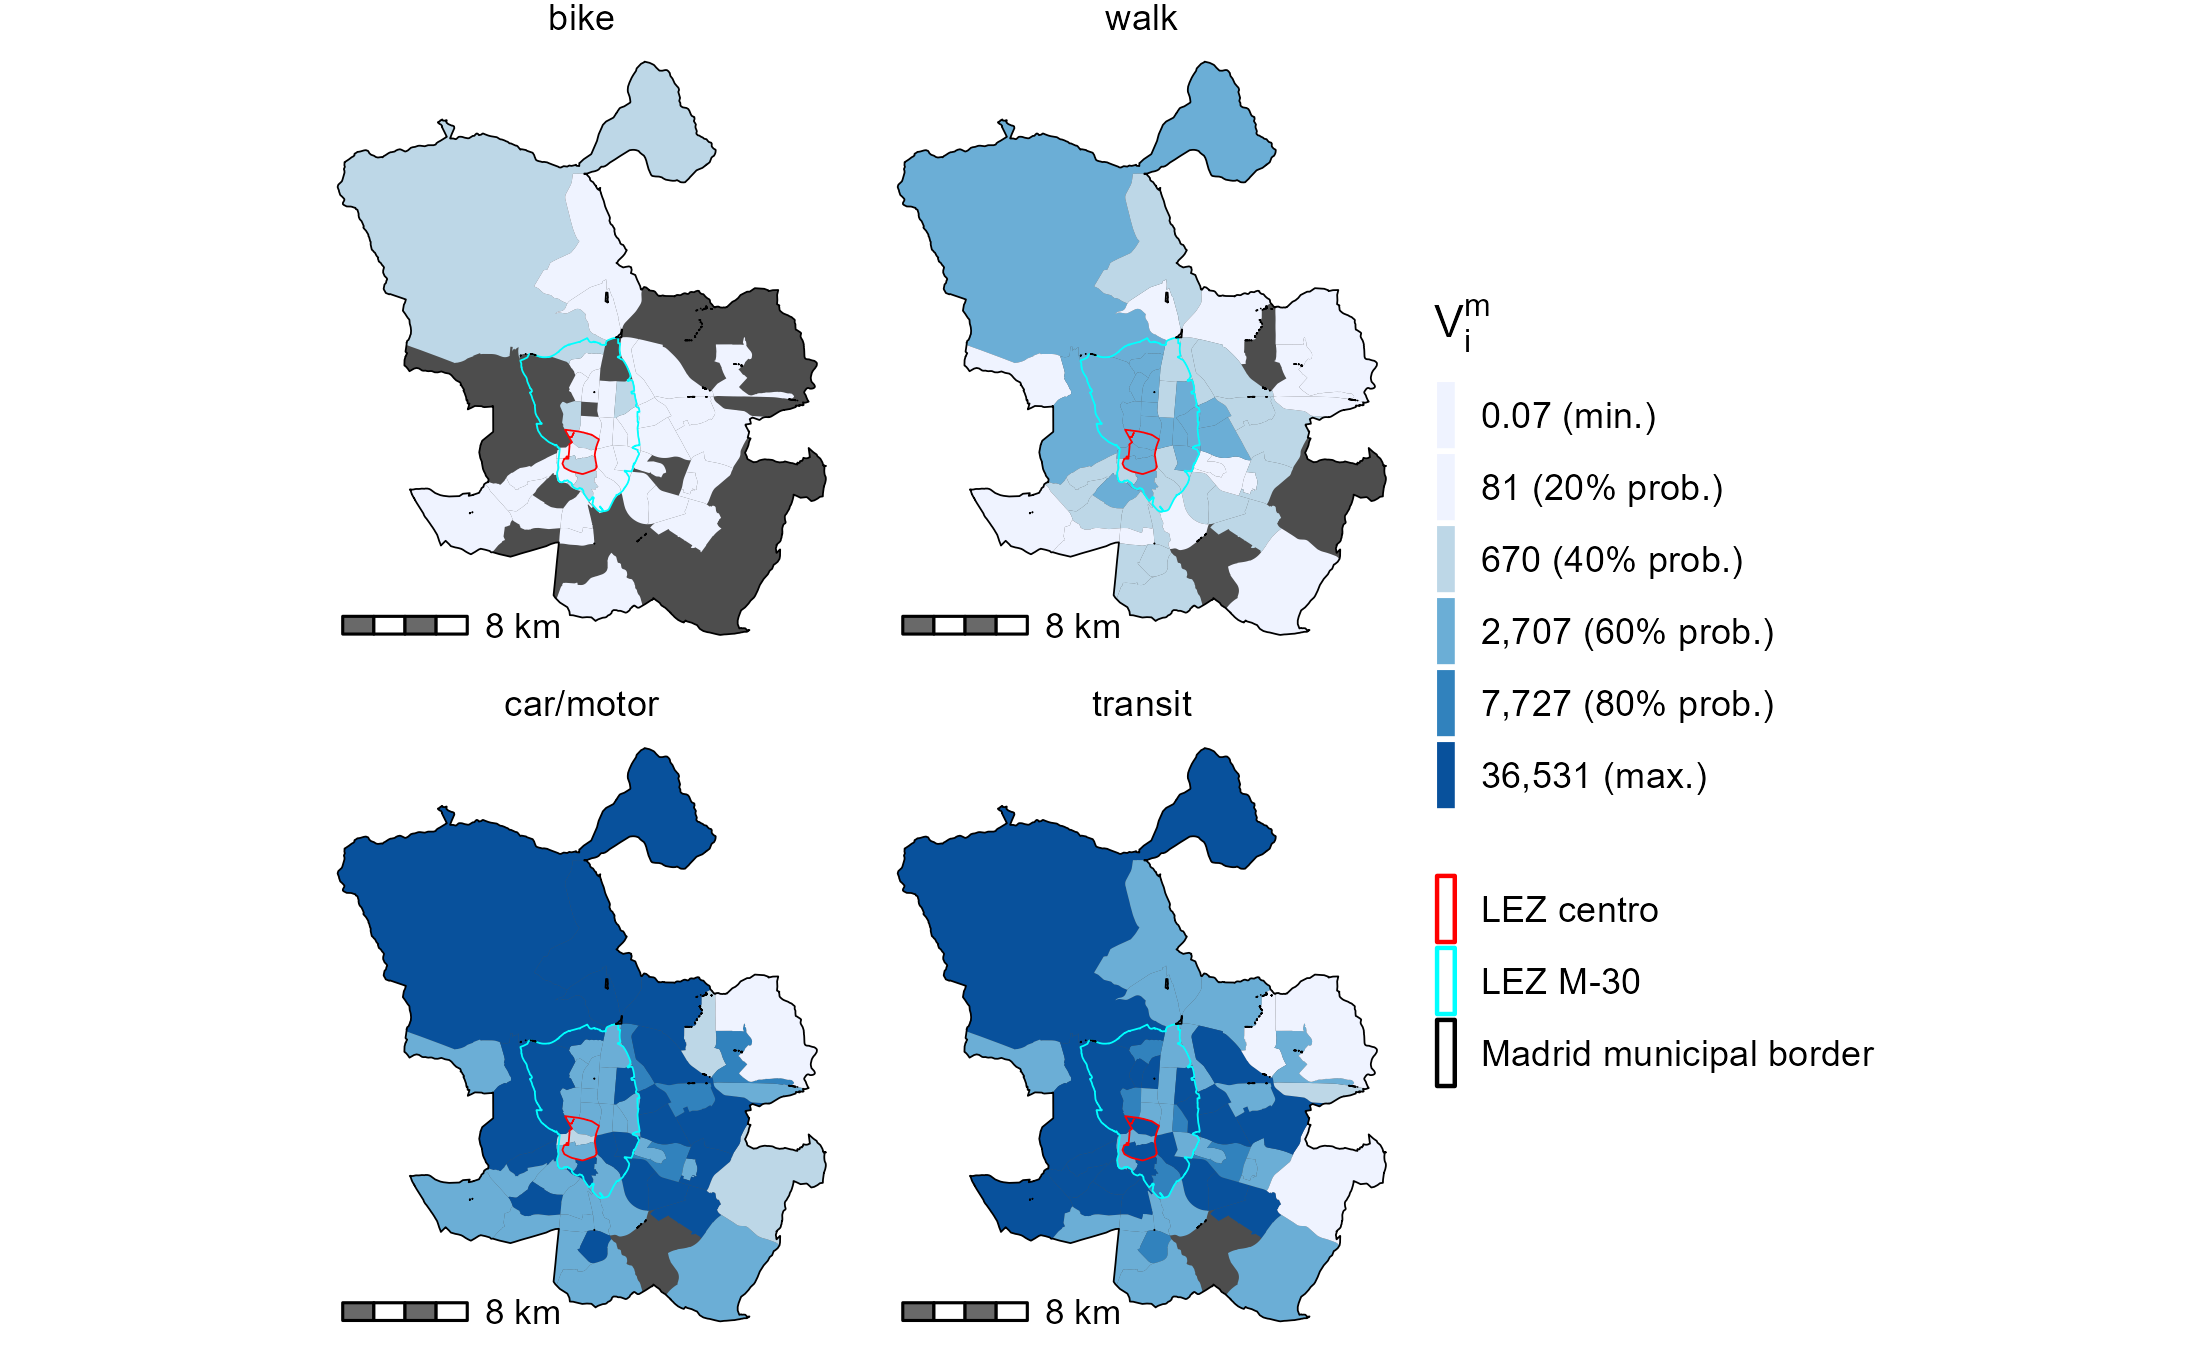
\includegraphics[width=1\linewidth]{images/SA_im_V_zn208_plot} 
%DIFDELCMD < %%%
\DIFdelendFL \DIFaddbeginFL 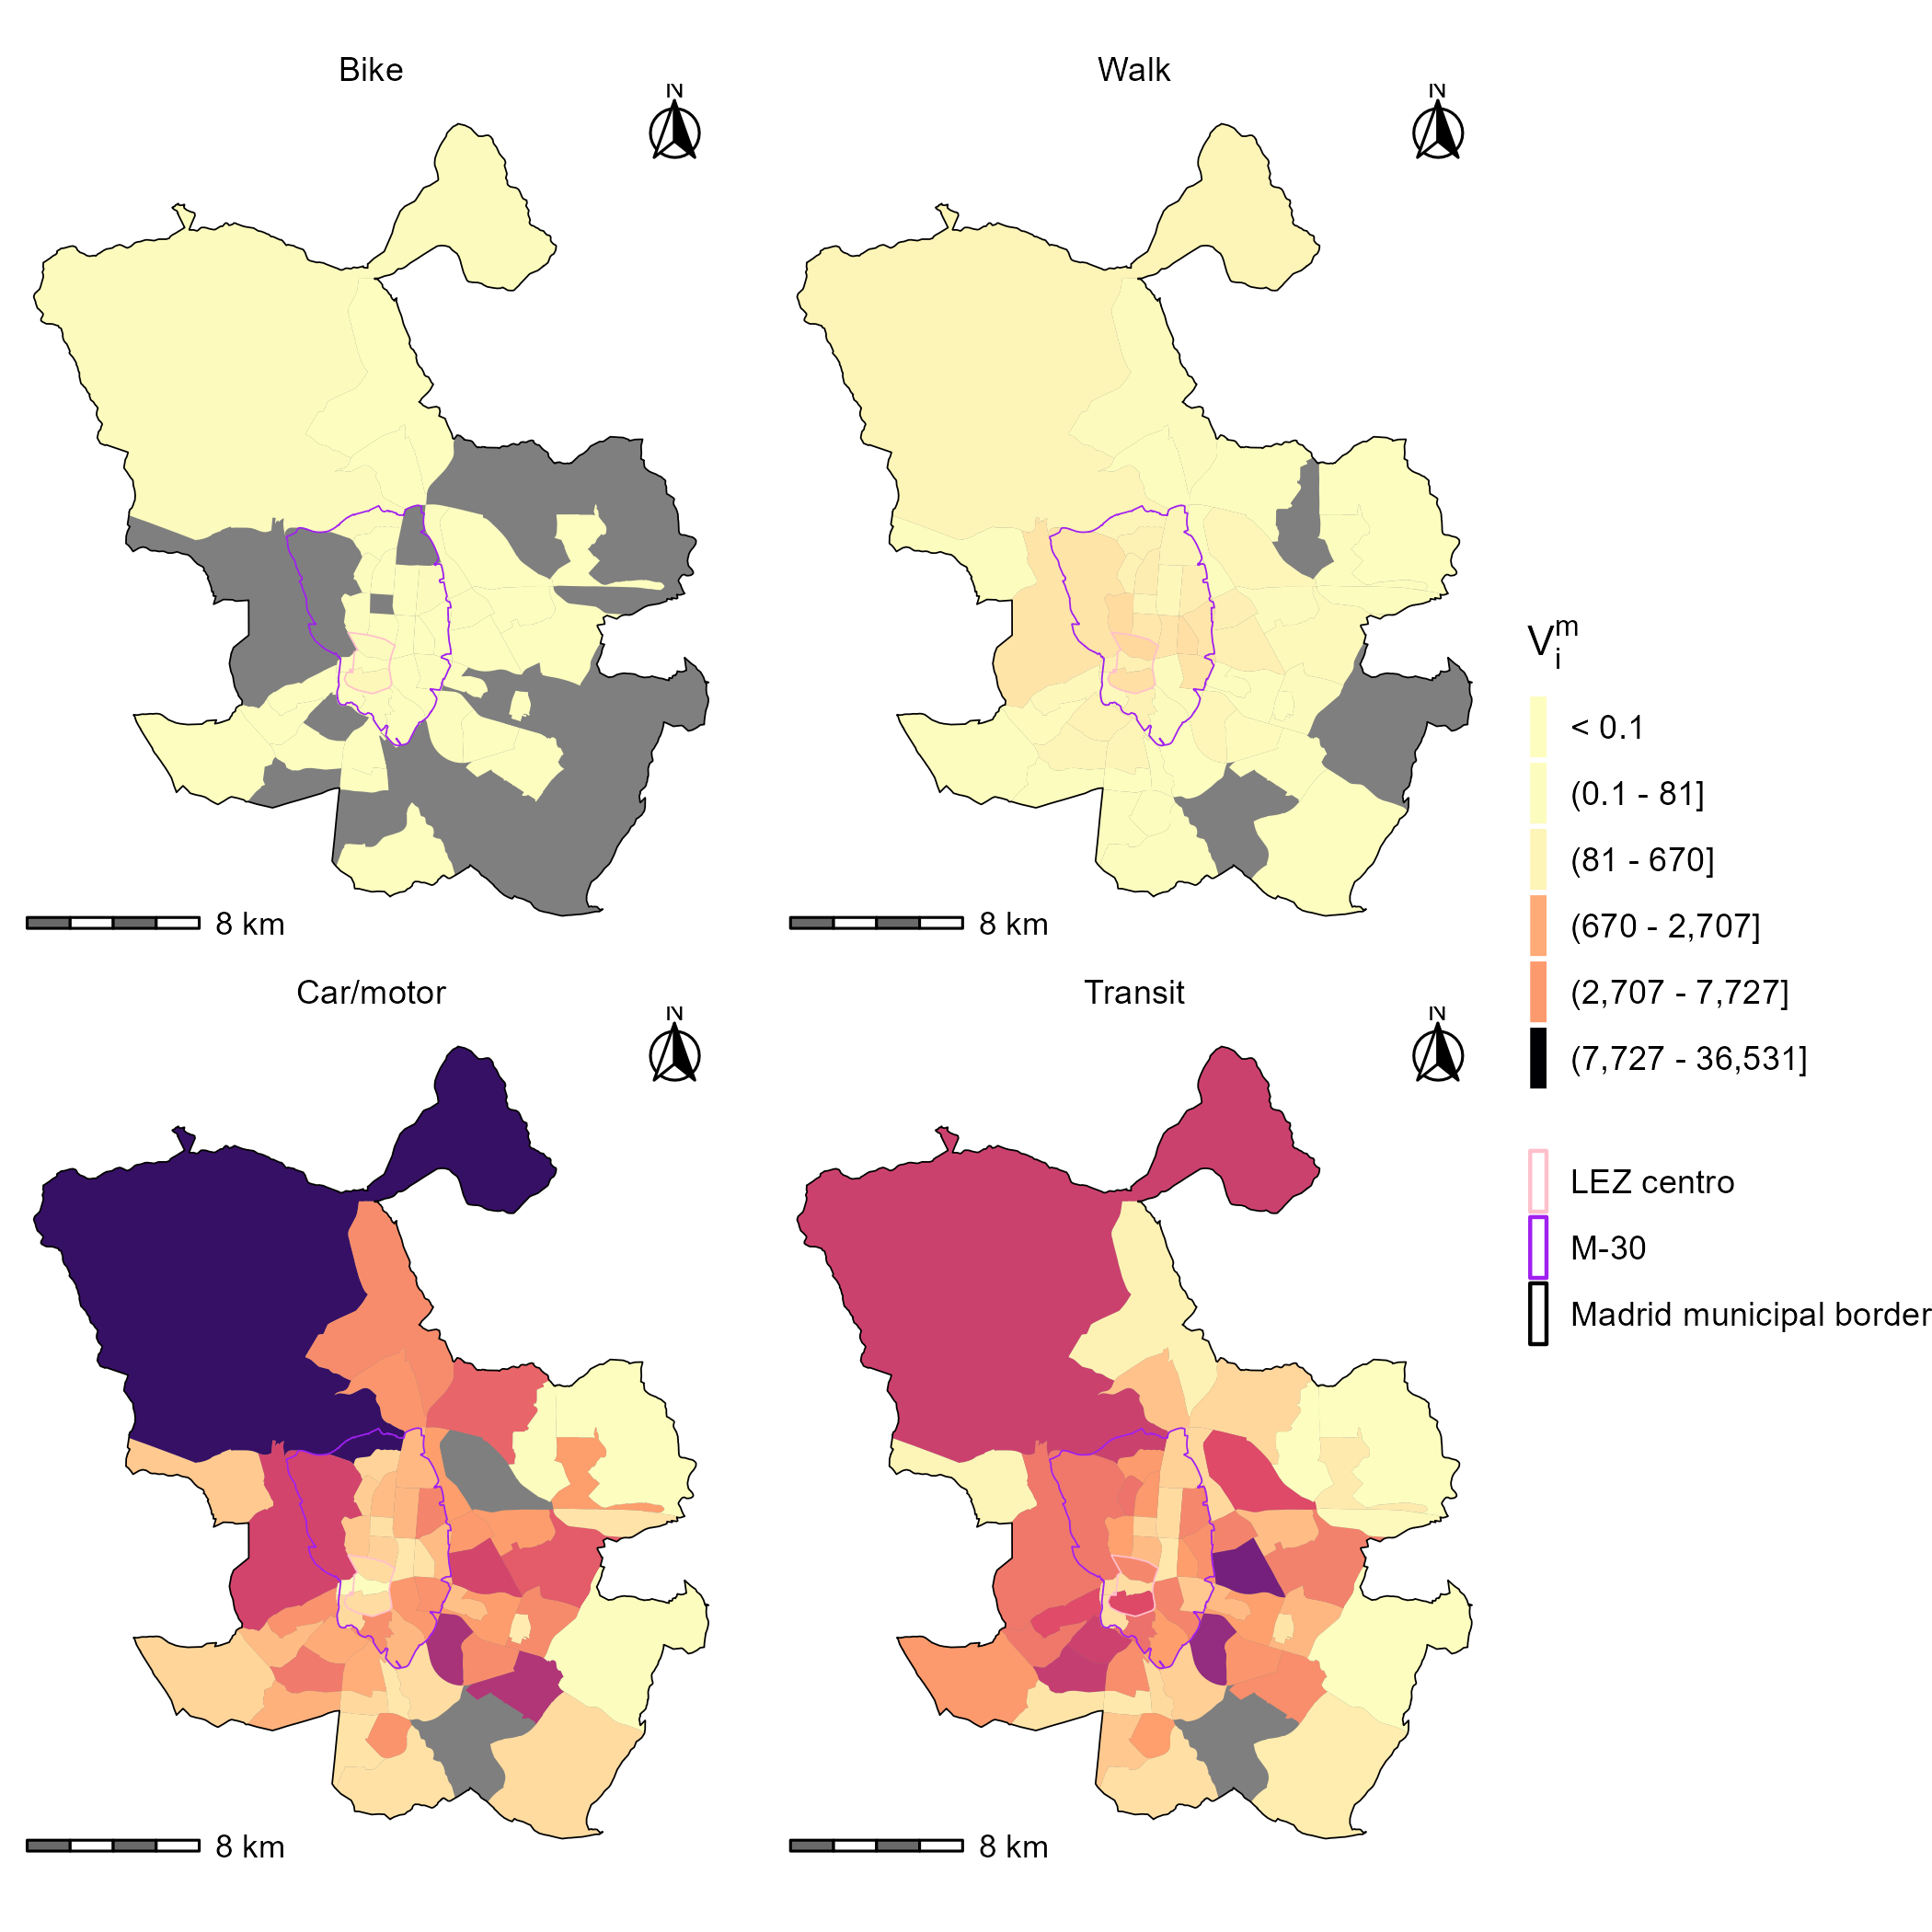
\includegraphics[width=0.85\linewidth]{images/Fig5} 
\DIFaddendFL 

}

\caption{\label{fig:Fig5} Spatial availability of \DIFdelbeginFL \DIFdelFL{job opportunities }\DIFdelendFL \DIFaddbeginFL \DIFaddFL{jobs }\DIFaddendFL per origin and mode $V_i^m$ in Madrid. \DIFdelbeginFL \DIFdelFL{Calculated using }\DIFdelendFL \DIFaddbeginFL \DIFaddFL{Grey TAZs have no population. Ranges of values in }\DIFaddendFL the \DIFdelbeginFL \DIFdelFL{home-to-work origin-destination flows from the 2018 travel survey}\DIFdelendFL \DIFaddbeginFL \DIFaddFL{legend are quintiles}\DIFaddendFL .}\label{fig:SA-m-plot}
\end{figure}

\DIFaddbegin \DIFadd{In the figure, }\DIFaddend \(V_i^m\) is a proportion of the total number of \DIFdelbegin \DIFdel{the }\DIFdelend 847,574
jobs in the region\DIFdelbegin \DIFdel{and is visualized in Figure \ref{fig:Fig5}}\DIFdelend . Since \(V_i^m\) is calculated based on the
\DIFdelbegin \DIFdel{likelihood of travel from observed home-to-work
journeys}\DIFdelend \DIFaddbegin \DIFadd{population of workers and the distribution of jobs}\DIFaddend , the values can be
understood as the number of full-time jobs that are spatially available
to \DIFdelbegin \DIFdel{the }\DIFdelend full-time \DIFdelbegin \DIFdel{working population }\DIFdelend \DIFaddbegin \DIFadd{workers }\DIFaddend at that \(i\) \DIFdelbegin \DIFdel{and their associated }\DIFdelend \DIFaddbegin \DIFadd{traveling by mode }\DIFaddend \(m\), relative to
all the jobs in the city. \DIFdelbegin \DIFdel{\(V_i^m\) is the number of jobs that are }\emph{\DIFdel{spatially available}} %DIFAUXCMD
\DIFdel{to a
\(m\)-using population located at \(i\), relative to the travel
impedance and size of }\emph{\DIFdel{all}} %DIFAUXCMD
\DIFdel{populations in the region.
}%DIFDELCMD < 

%DIFDELCMD < %%%
\DIFdel{Notable are the }\DIFdelend \DIFaddbegin \DIFadd{There are noticeable }\DIFaddend differences in the
magnitude of \(V_i^m\) between modes \DIFaddbegin \DIFadd{as seen }\DIFaddend in Figure \ref{fig:Fig5}.
The majority of \(V_i^m\) \DIFaddbegin \DIFadd{(which is to say of spatially available jobs)
are allocated to workers travelling by car and transit. In a way, this
}\DIFaddend is \DIFdelbegin \DIFdel{allocated }\DIFdelend to \DIFdelbegin \DIFdel{car-
and transit- using populations. This is to }\DIFdelend be expected \DIFdelbegin \DIFdel{, as the
population that commutes using these modes represents }\DIFdelend \DIFaddbegin \DIFadd{since users of these modes represent }\DIFaddend 84.1\% of the
total population. \DIFdelbegin \DIFdel{Differences }\DIFdelend \DIFaddbegin \DIFadd{However, the ability to travel at greater speeds also
impacts these results. Furthermore, differences }\DIFaddend in \(V_i^m\) values
within \DIFdelbegin \DIFdel{mode-using
populations also exist : car-using populations }\DIFdelend \DIFaddbegin \DIFadd{modes also exist in space: car users }\DIFaddend outside of the M-30 region
appear to \DIFdelbegin \DIFdel{have greater \(V_i^m\) values}\DIFdelend \DIFaddbegin \DIFadd{enjoy greater spatial availability}\DIFaddend , while some \DIFdelbegin \DIFdel{\(i\) areas }\DIFdelend \DIFaddbegin \DIFadd{zones }\DIFaddend inside
the M-30 \DIFdelbegin \DIFdel{appear to have higher \(V_i^m\) values for the transit-using
populations}\DIFdelend \DIFaddbegin \DIFadd{to have greater spatial availability for transit}\DIFaddend . Overall, the
magnitude of \(V_i^m\) values for \DIFdelbegin \DIFdel{the bikers
and walkers }\DIFdelend \DIFaddbegin \DIFadd{cyclists and pedestrians }\DIFaddend are lower
than \DIFaddbegin \DIFadd{for }\DIFaddend car and transit but the highest \DIFaddbegin \DIFadd{values of }\DIFaddend \(V_i^{bike}\) and
\(V_i^{walk}\) \DIFdelbegin \DIFdel{values }\DIFdelend tend to be \DIFdelbegin \DIFdel{allotted to \(i\)s
}\DIFdelend \DIFaddbegin \DIFadd{found in zones }\DIFaddend within the M-30 and \DIFdelbegin \DIFdel{\(i\)s that have higher \(V_i^{transit}\) values}\DIFdelend \DIFaddbegin \DIFadd{origins
with higher spatial availability by transit}\DIFaddend .

The differences between the \DIFdelbegin \DIFdel{mode-using population and their mode-specific spatial availability }\DIFdelend \DIFaddbegin \DIFadd{shares of modes and their shares of
spatially available opportunities }\DIFaddend highlights the competitive advantage
\DIFdelbegin \DIFdel{offered to certain modesin certain spatial extents. As
summarized }\DIFdelend \DIFaddbegin \DIFadd{of certain modes, although this effect is not geographically uniform. As
seen }\DIFaddend in the left-most columns \DIFdelbegin \DIFdel{in }\DIFdelend \DIFaddbegin \DIFadd{of }\DIFaddend Figure \ref{fig:Fig6}, \DIFdelbegin \DIFdel{the }\DIFdelend \DIFaddbegin \DIFadd{users of
}\DIFaddend `car/motor' and `transit' \DIFdelbegin \DIFdel{populations represent a combined }\DIFdelend \DIFaddbegin \DIFadd{together can avail }\DIFaddend 95.3\% of \DIFdelbegin \DIFdel{the total spatial
availability }\DIFdelend \DIFaddbegin \DIFadd{all jobs }\DIFaddend in the
city \DIFaddbegin \DIFadd{(Spatial Availability by Mode)}\DIFaddend . However, \DIFdelbegin \DIFdel{the `}\DIFdelend car/motor \DIFdelbegin \DIFdel{' using population is
allocated disproportionately more }\DIFdelend \DIFaddbegin \DIFadd{users have a
disproportionate share of }\DIFaddend \(V_i^m\) \DIFdelbegin \DIFdel{than its size compared to the transit-using population . The car-using and transit-using population }\DIFdelend \DIFaddbegin \DIFadd{relative to the population of users
of this mode (Population by Mode), compared to opportunities that are
spatially available to transit users. The combined population of car and
transit users }\DIFaddend is 36.6\% and 47.5\% respectively, but \DIFdelbegin \DIFdel{is }\DIFdelend \DIFaddbegin \DIFadd{these populations
are }\DIFaddend allocated 48.0\% and 47.3\% respectively, of the city's \DIFdelbegin \DIFdel{spatial availability}\DIFdelend \DIFaddbegin \DIFadd{jobs}\DIFaddend . When
treating the number of opportunities that can be reached as a finite
value (total: 847,574 opportunities), fewer opportunities are \DIFdelbegin \DIFdel{spatial availability to the lesser competitive modes-using populations, in this case }\DIFdelend \DIFaddbegin \DIFadd{spatially
available to slower modes (i.e., }\DIFaddend walking and cycling\DIFaddbegin \DIFadd{), even taking into
account that their share is smaller overall}\DIFaddend . These modes are \DIFdelbegin \DIFdel{less competitive }\DIFdelend \DIFaddbegin \DIFadd{at a
disadvantage }\DIFaddend as a result of: \DIFdelbegin \DIFdel{their lower
travel impedance values at longer travel times }\DIFdelend \DIFaddbegin \DIFadd{the travel impedance for longer trips }\DIFaddend (see
Figure \ref{fig:Fig4}\DIFdelbegin \DIFdel{at travel times beyond \textasciitilde30 minutes)}\DIFdelend ; their low population values values overall; and
\DIFdelbegin \DIFdel{higher populations present }\DIFdelend \DIFaddbegin \DIFadd{larger populations }\DIFaddend in origins with high \DIFdelbegin \DIFdel{motorized mode commuting}\DIFdelend \DIFaddbegin \DIFadd{shares of travel by motorized
modes}\DIFaddend . These factors all contribute to the the car/motor mode being most
advantaged in capturing spatially available job opportunities overall.

\begin{figure}

{\centering \DIFdelbeginFL %DIFDELCMD < 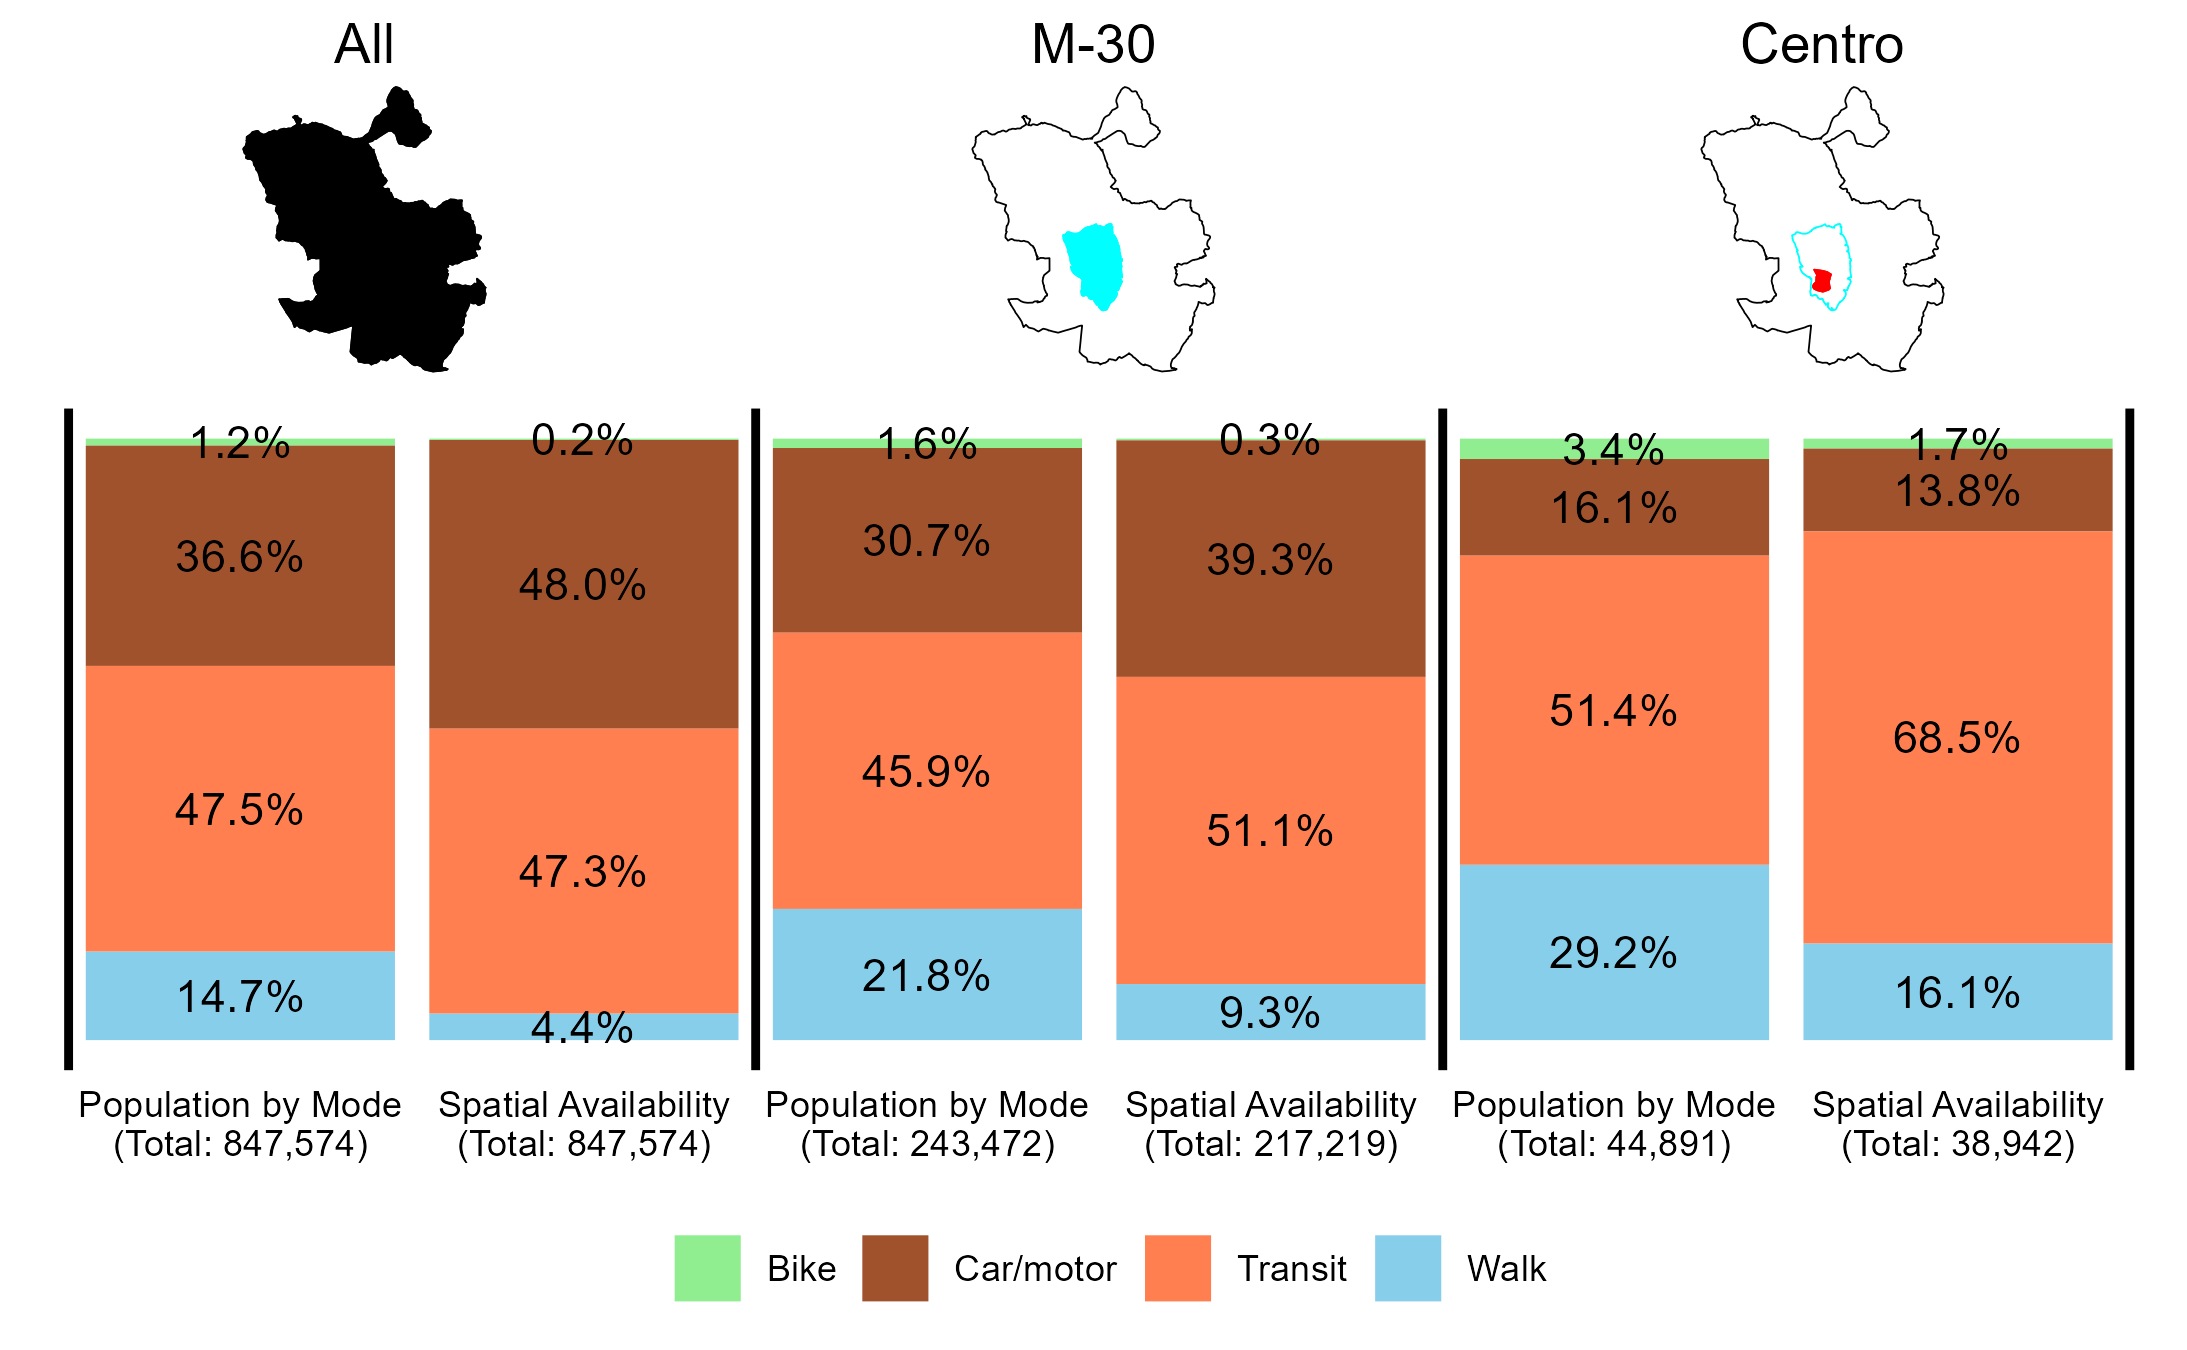
\includegraphics[width=1\linewidth]{images/modal_V_comps_4plot} 
%DIFDELCMD < %%%
\DIFdelendFL \DIFaddbeginFL 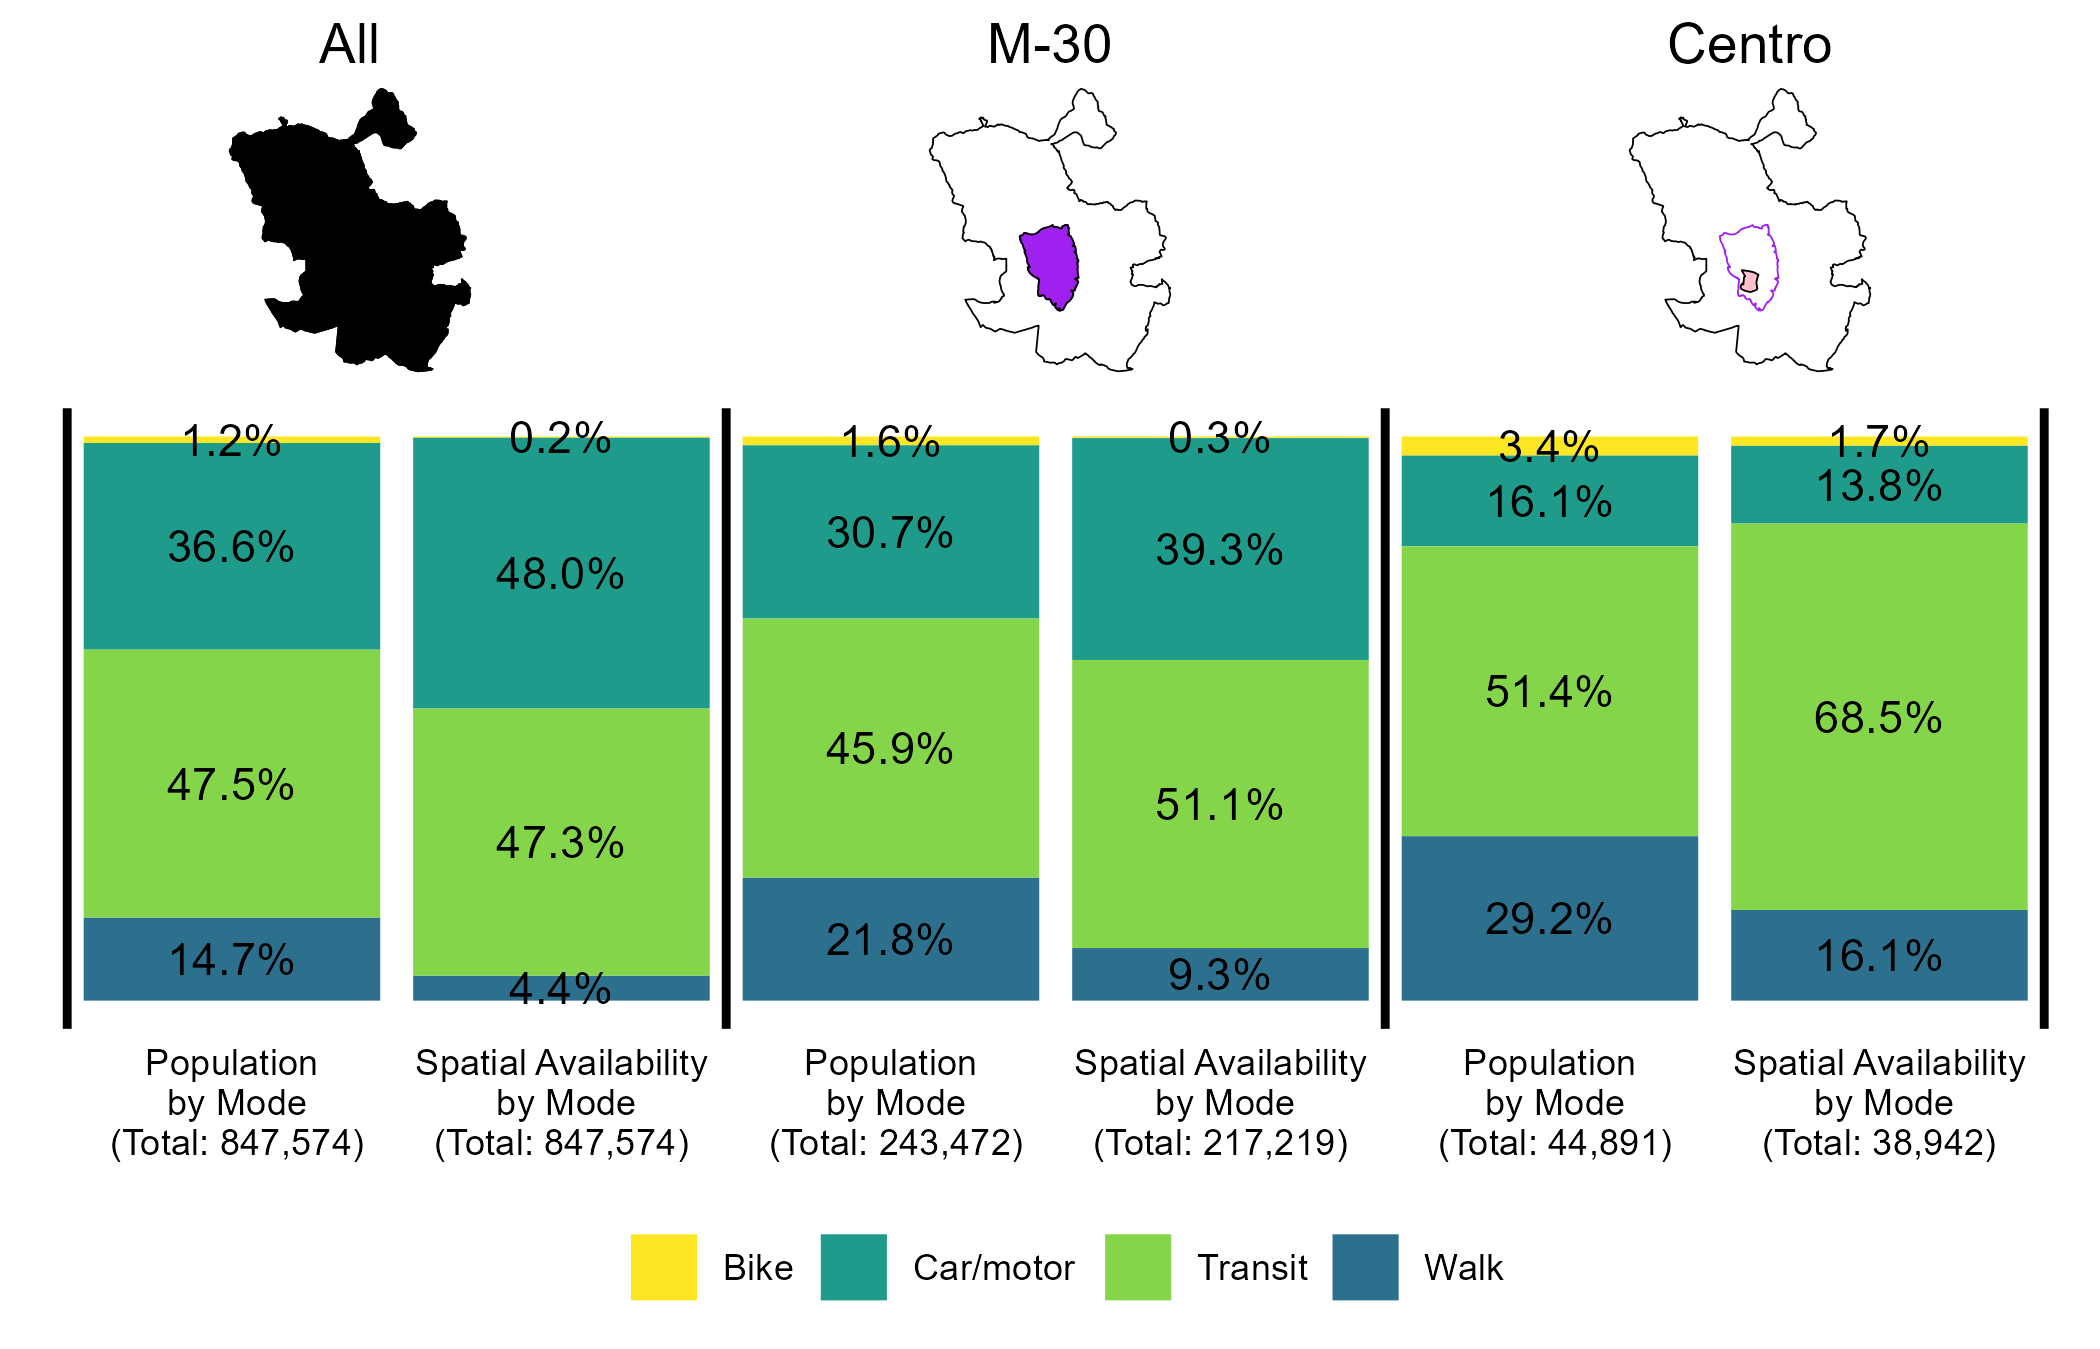
\includegraphics[width=0.85\linewidth]{images/Fig6} 
\DIFaddendFL 

}

\caption{\label{fig:Fig6} \DIFdelbeginFL \DIFdelFL{Displays the proportion }\DIFdelendFL \DIFaddbeginFL \DIFaddFL{Proportion }\DIFaddendFL of \DIFdelbeginFL \DIFdelFL{the working }\DIFdelendFL population by mode and spatial availability of \DIFdelbeginFL \DIFdelFL{job opportunities }\DIFdelendFL \DIFaddbeginFL \DIFaddFL{jobs }\DIFaddendFL by mode aggregated for three \DIFdelbeginFL \DIFdelFL{spatial }\DIFdelendFL areas. From left to right, the city of Madrid (All), the area within the M-30 highway (M-30), the area within the Centro region (Centro).}\label{fig:modal-V-comps-plot}
\end{figure}

\DIFdelbegin \DIFdel{There are spatial variations in the competitive advantage of the car-using populations. The proportion of car-using population in the Centro is smaller and has higher travel impedance values relative to the inputs in other areas and mode-using populations. The LEZ Centro
implementation further restricts the car-advantage as it shifted more
than half of all car trips into the LEZ to another mode }%DIFDELCMD < {[}%%%
\DIFdel{25}%DIFDELCMD < {]}%%%
\DIFdel{. This
restriction decreased the number of car-using population from \(i\)s
going into the LEZ Centro (an area with }\DIFdelend \DIFaddbegin \DIFadd{The big picture demonstrates how car is the most advantageous mode,
however it is interesting to notice that this advantage appears to be
blunted by the LEZ. Unlike the results for the whole city and even
within the M-30 ring, the proportion of car users in Centro is larger
than the proportion of opportunities spatially available to them. The
restriction on cars in effect reduces competition by this mode, and
leads to a relative increment of the mass effect of the modes allowed
within the LEZ, which also contains }\DIFaddend a large number of jobs \DIFdelbegin \DIFdel{overall,
}\DIFdelend \DIFaddbegin \DIFadd{(}\DIFaddend see Figure
\ref{fig:Fig2})\DIFdelbegin \DIFdel{, thus increasing the mass effect for non-car
modes and resulting in proportionally higher \(v_i^m\) values for
non-car modes. As such, the lower amount of access to opportunities by
car-mode allows more opportunities in the LEZ to be available by
populations using other modes.
}%DIFDELCMD < 

%DIFDELCMD < %%%
\DIFdelend \DIFaddbegin \DIFadd{. }\DIFaddend As summarized in the two right-most columns in Figure
\ref{fig:Fig6}, the proportion of \DIFdelbegin \DIFdel{spatial availability allocated to the car-using
population in
the Centro }\DIFdelend \DIFaddbegin \DIFadd{jobs spatially available to car in
Centro is }\DIFaddend (13.8\% or 5,373 opportunities). \DIFdelbegin \DIFdel{As a
comparative }\DIFdelend \DIFaddbegin \DIFadd{For }\DIFaddend reference, this is less
than the proportion of the \DIFdelbegin \DIFdel{car-using
population in the }\DIFdelend \DIFaddbegin \DIFadd{car users in }\DIFaddend Centro (16.1\%), evidently less
then the proportion of \DIFdelbegin \DIFdel{car-using population }\DIFdelend \DIFaddbegin \DIFadd{car users }\DIFaddend in the city, and is the opposite of the
\DIFdelbegin \DIFdel{trend
overall }\DIFdelend \DIFaddbegin \DIFadd{overall trend }\DIFaddend (left-most columns) and within the M-30 (middle columns).
\DIFdelbegin \DIFdel{More
opportunities are spatial availability }\DIFdelend \DIFaddbegin 

\DIFadd{It is also clear that more opportunities are spatially available }\DIFaddend to
non-car \DIFdelbegin \DIFdel{using populations
within the Centro, particularly transit-using populations (68.5\% of spatially available jobs in the
Centro despite representing 51.4\% of the population in the Centro and 47.5\% in the cityoverall). }%DIFDELCMD < 

%DIFDELCMD < %%%
\DIFdel{From }\DIFdelend \DIFaddbegin \DIFadd{users within Centro. In the case of active travel, the
proportions of cyclists and walkers within LEZ Centro still exceeds the
proportions of jobs spatially available to them --- however, the
disparity is drastically reduced compared to the rest of the city. As
seen in }\DIFaddend Figure \ref{fig:Fig6}, \DIFdelbegin \DIFdel{it is also summarized that }\DIFdelend there is a higher proportion of
opportunities \DIFaddbegin \DIFadd{that are }\DIFaddend spatially available to \DIFdelbegin \DIFdel{walking and cycling
populations in the }\DIFdelend \DIFaddbegin \DIFadd{pedestrians and cyclists
in }\DIFaddend Centro than in the City overall and in \DIFdelbegin \DIFdel{all }\DIFdelend areas within the M-30.
Notably, within \DIFdelbegin \DIFdel{the }\DIFdelend Centro, 1.7\% and 16.1\% of opportunities are spatially
available to bike and walk modes respectively, while their populations
represent \DIFdelbegin \DIFdel{smaller proportions of
}\DIFdelend 1.2\% and 14.7\% of the population\DIFdelbegin \DIFdel{overall. Though the proportion of spatial availability for these mode-using populations is still lower
than the proportion of mode-using population located in the Centro, these modes are
more competitive within the Centro than outside of the
Centro }\DIFdelend . \DIFdelbegin \DIFdel{By restricting the more competitive carmode through the LEZ, the advantage in the spatial availability of opportunities afforded to
the otherwise lesser competitive modes is made apparent}\DIFdelend \DIFaddbegin \DIFadd{By restricting the ability
of cars to enter Centro, the LEZ seems to contribute to leveling the
playing field for slower modes, in particular cycling and walking, but
also transit. As seen in the Figure \ref{fig:Fig6}, transit users are
generally close to parity across the region, with nearly as many
spatially available jobs as transit users. Still, this mode has the
greatest advantage in LEZ Centro with 68.5\% of spatially available jobs
in Centro for 51.4\% of transit users in Centro. This result makes
intuitive sense: after car, it is the mode with the greatest range, and
unlike car it is unrestricted in the LEZ Centro}\DIFaddend .

The spatial differences in the competitive dis/advantage of spatial
availability between modes can also be visualized \DIFdelbegin \DIFdel{per origin}\DIFdelend \DIFaddbegin \DIFadd{at a finer level of
granularity}\DIFaddend . Figure \ref{fig:Fig7} \DIFdelbegin \DIFdel{visualizes }\DIFdelend \DIFaddbegin \DIFadd{shows }\DIFaddend \(v_i^m\), the spatial
availability \(V_i^m\) divided by the \DIFdelbegin \DIFdel{mode-population.
}\DIFdelend \DIFaddbegin \DIFadd{population of users of \(m\).
Values of }\DIFaddend \(v_i^m\) \DIFdelbegin \DIFdel{values above 1 are represented
in increasing red shades , values below 1 are represented in increasingly
green shades , and values equal to 1 are white. These plots illustrates
the discussion of the disproportionately high over-allocation of spatial
availability relative to the mode-using population in many of the
origins for the car/motor mode }\DIFdelend \DIFaddbegin \DIFadd{below one are shown in shades of orange, and
indicate TAZs with less than one spatially available opportunity per
capita for the mode. Values above one are shown in shades of green, and
indicate TAZs with more than one spatially available opportunity per
capita for the mode. The highest spatial availability per capita (shown
in blue) is for car users in a zone northeast just beyond the M-30.
These plots illustrate in unambiguous fashion, and in a quantity that is
comparable over space and time, the advantage in terms of spatial
availability of car for most of the city }\DIFaddend (bottom left plot, areas
denoted with green \(v_i^m\) values above \DIFdelbegin \DIFdel{1). These plots also visualize areas that
disproportionately capture lower spatial availability (under 1),
represented in shades of red. It can }\DIFdelend \DIFaddbegin \DIFadd{one). It can also }\DIFaddend be observed
that \DIFdelbegin \DIFdel{the transit-using
population's spatial availability to }\DIFdelend \DIFaddbegin \DIFadd{spatial availability of }\DIFaddend jobs is relatively \DIFdelbegin \DIFdel{balanced }\DIFdelend \DIFaddbegin \DIFadd{well balanced for
transit users over most of the regions }\DIFaddend (i.e., many zones are \DIFdelbegin \DIFdel{white), while the }\DIFdelend \DIFaddbegin \DIFadd{light
orange or light green). Spatial availability of jobs for }\DIFaddend non-motorized
modes\DIFdelbegin \DIFdel{\(v_i^m\) values
are }\DIFdelend \DIFaddbegin \DIFadd{, in contrast, is }\DIFaddend low (under \DIFdelbegin \DIFdel{1) overall}\DIFdelend \DIFaddbegin \DIFadd{one) overall, although less so within
LEZ Centro}\DIFaddend .

\begin{figure}

{\centering \DIFdelbeginFL %DIFDELCMD < 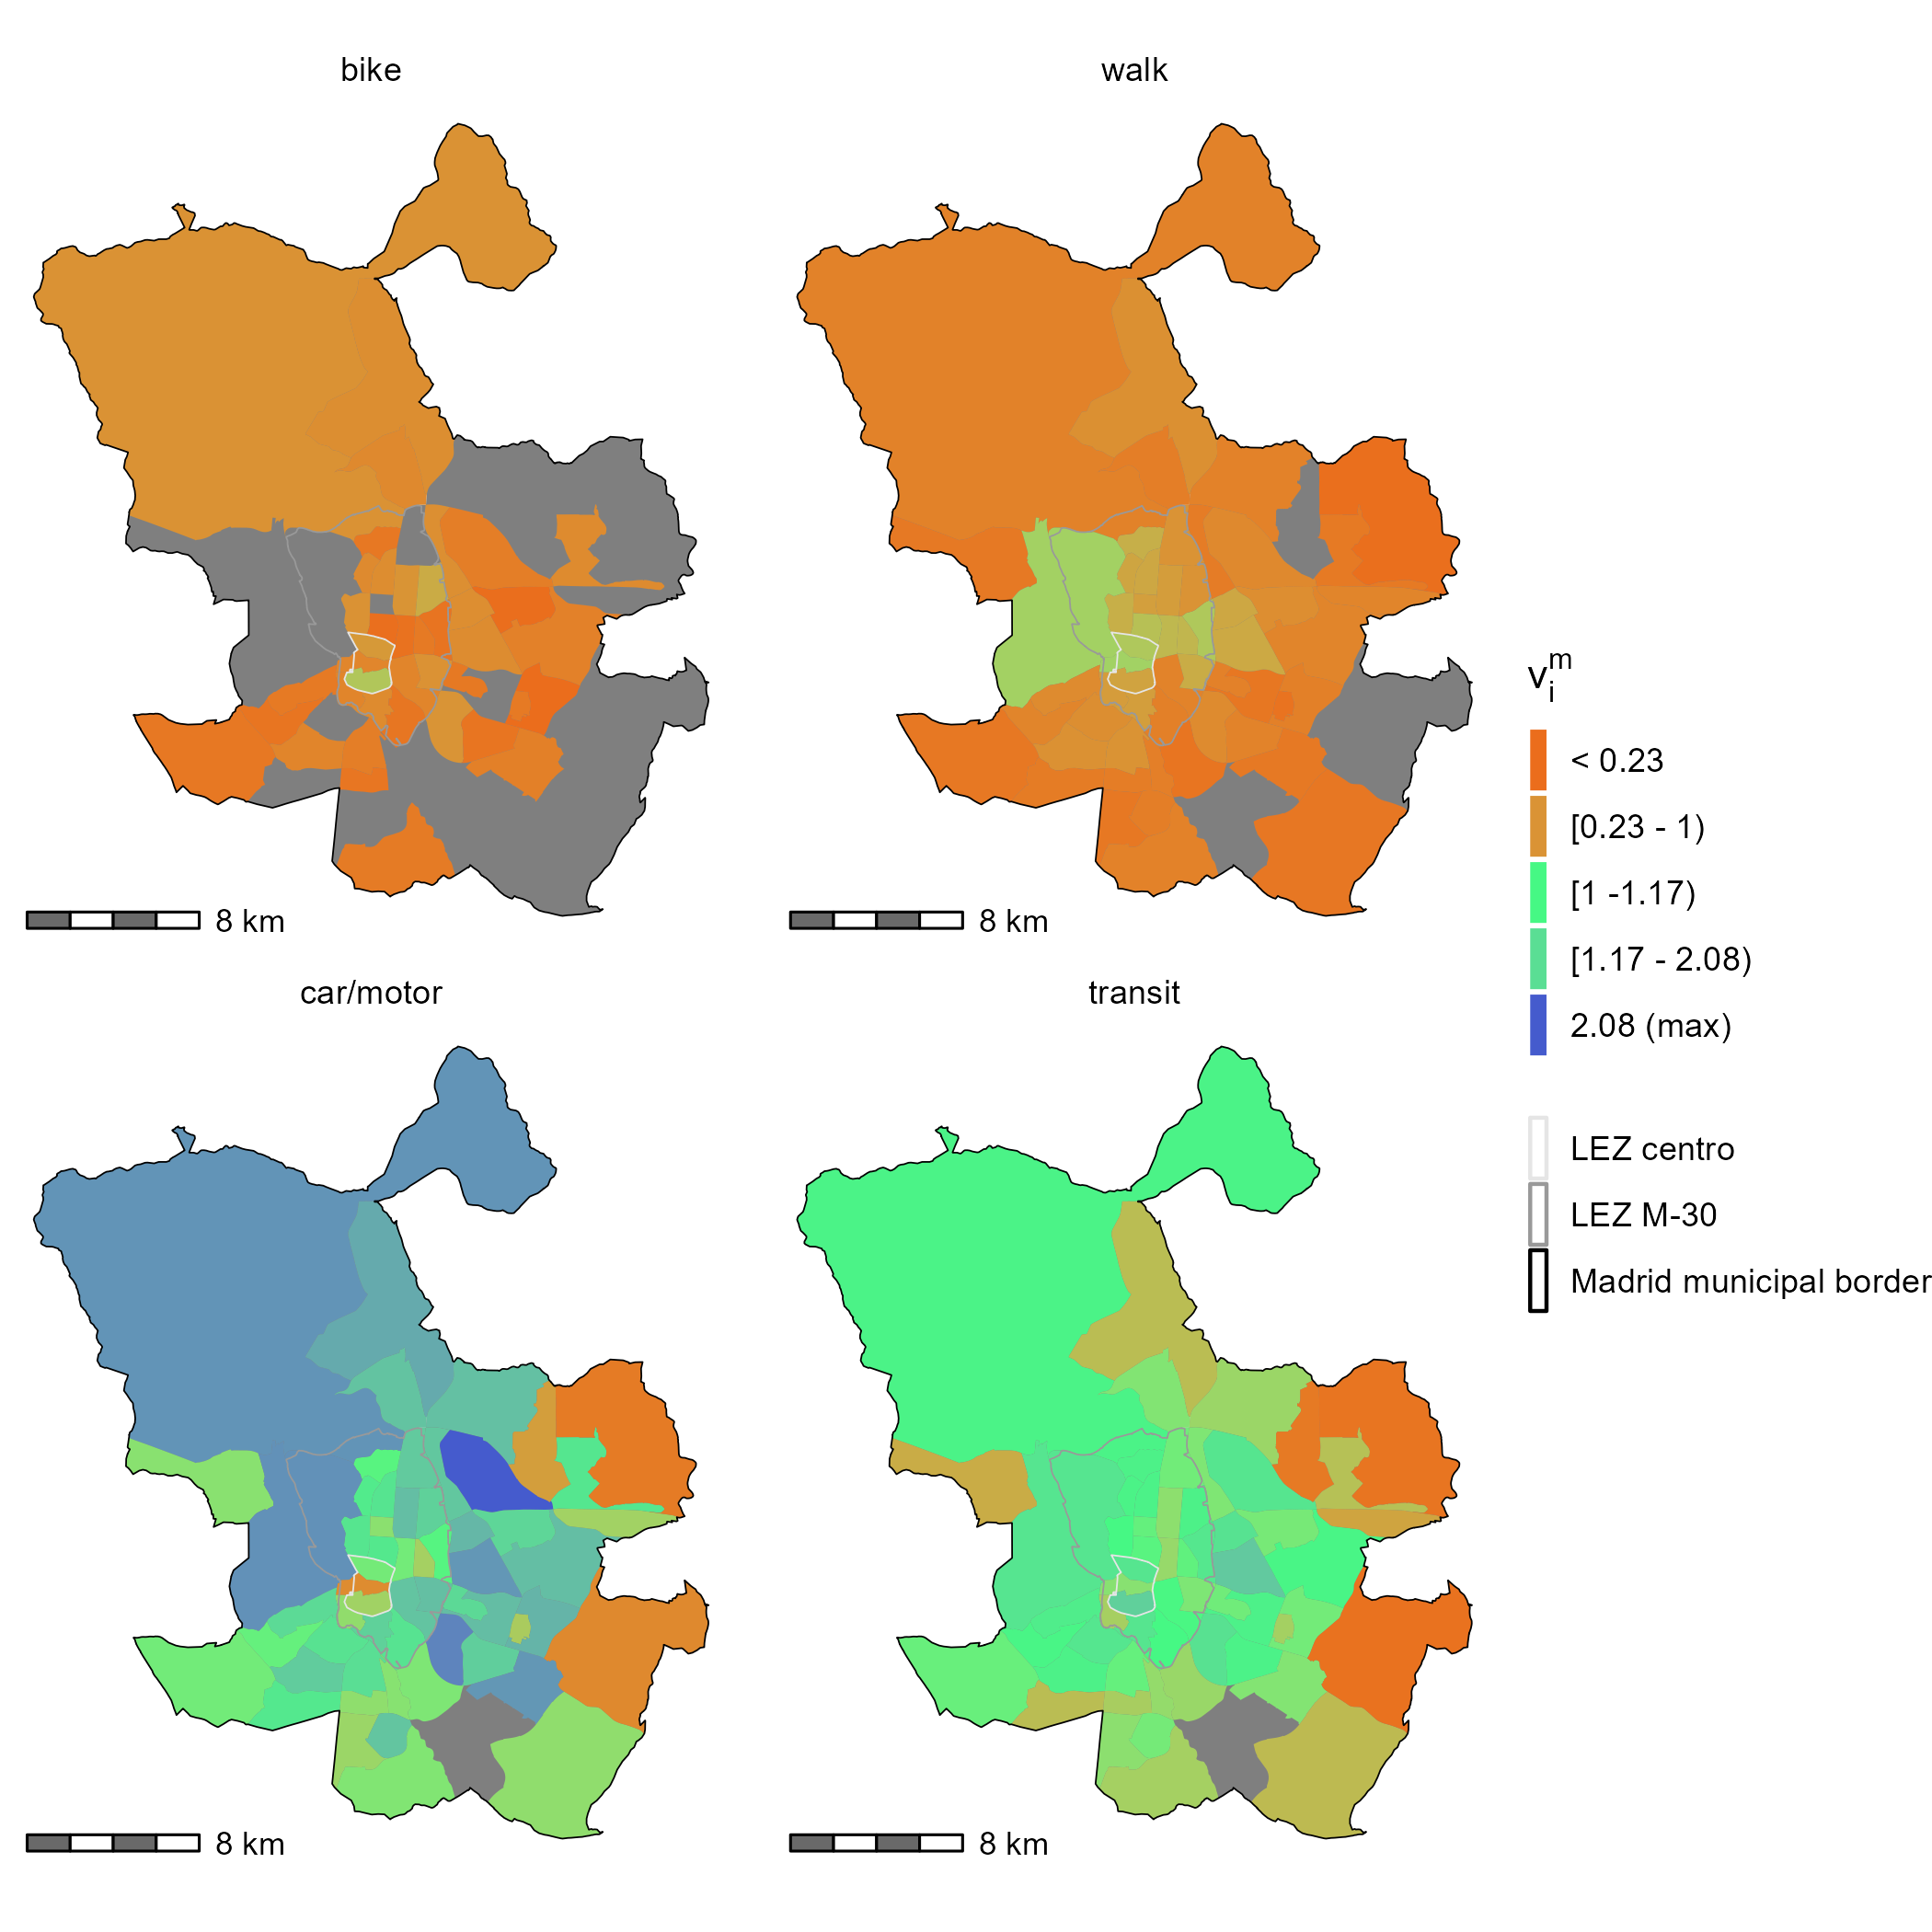
\includegraphics[width=1\linewidth]{images/SA_im_vv_zn208_plot} 
%DIFDELCMD < %%%
\DIFdelendFL \DIFaddbeginFL 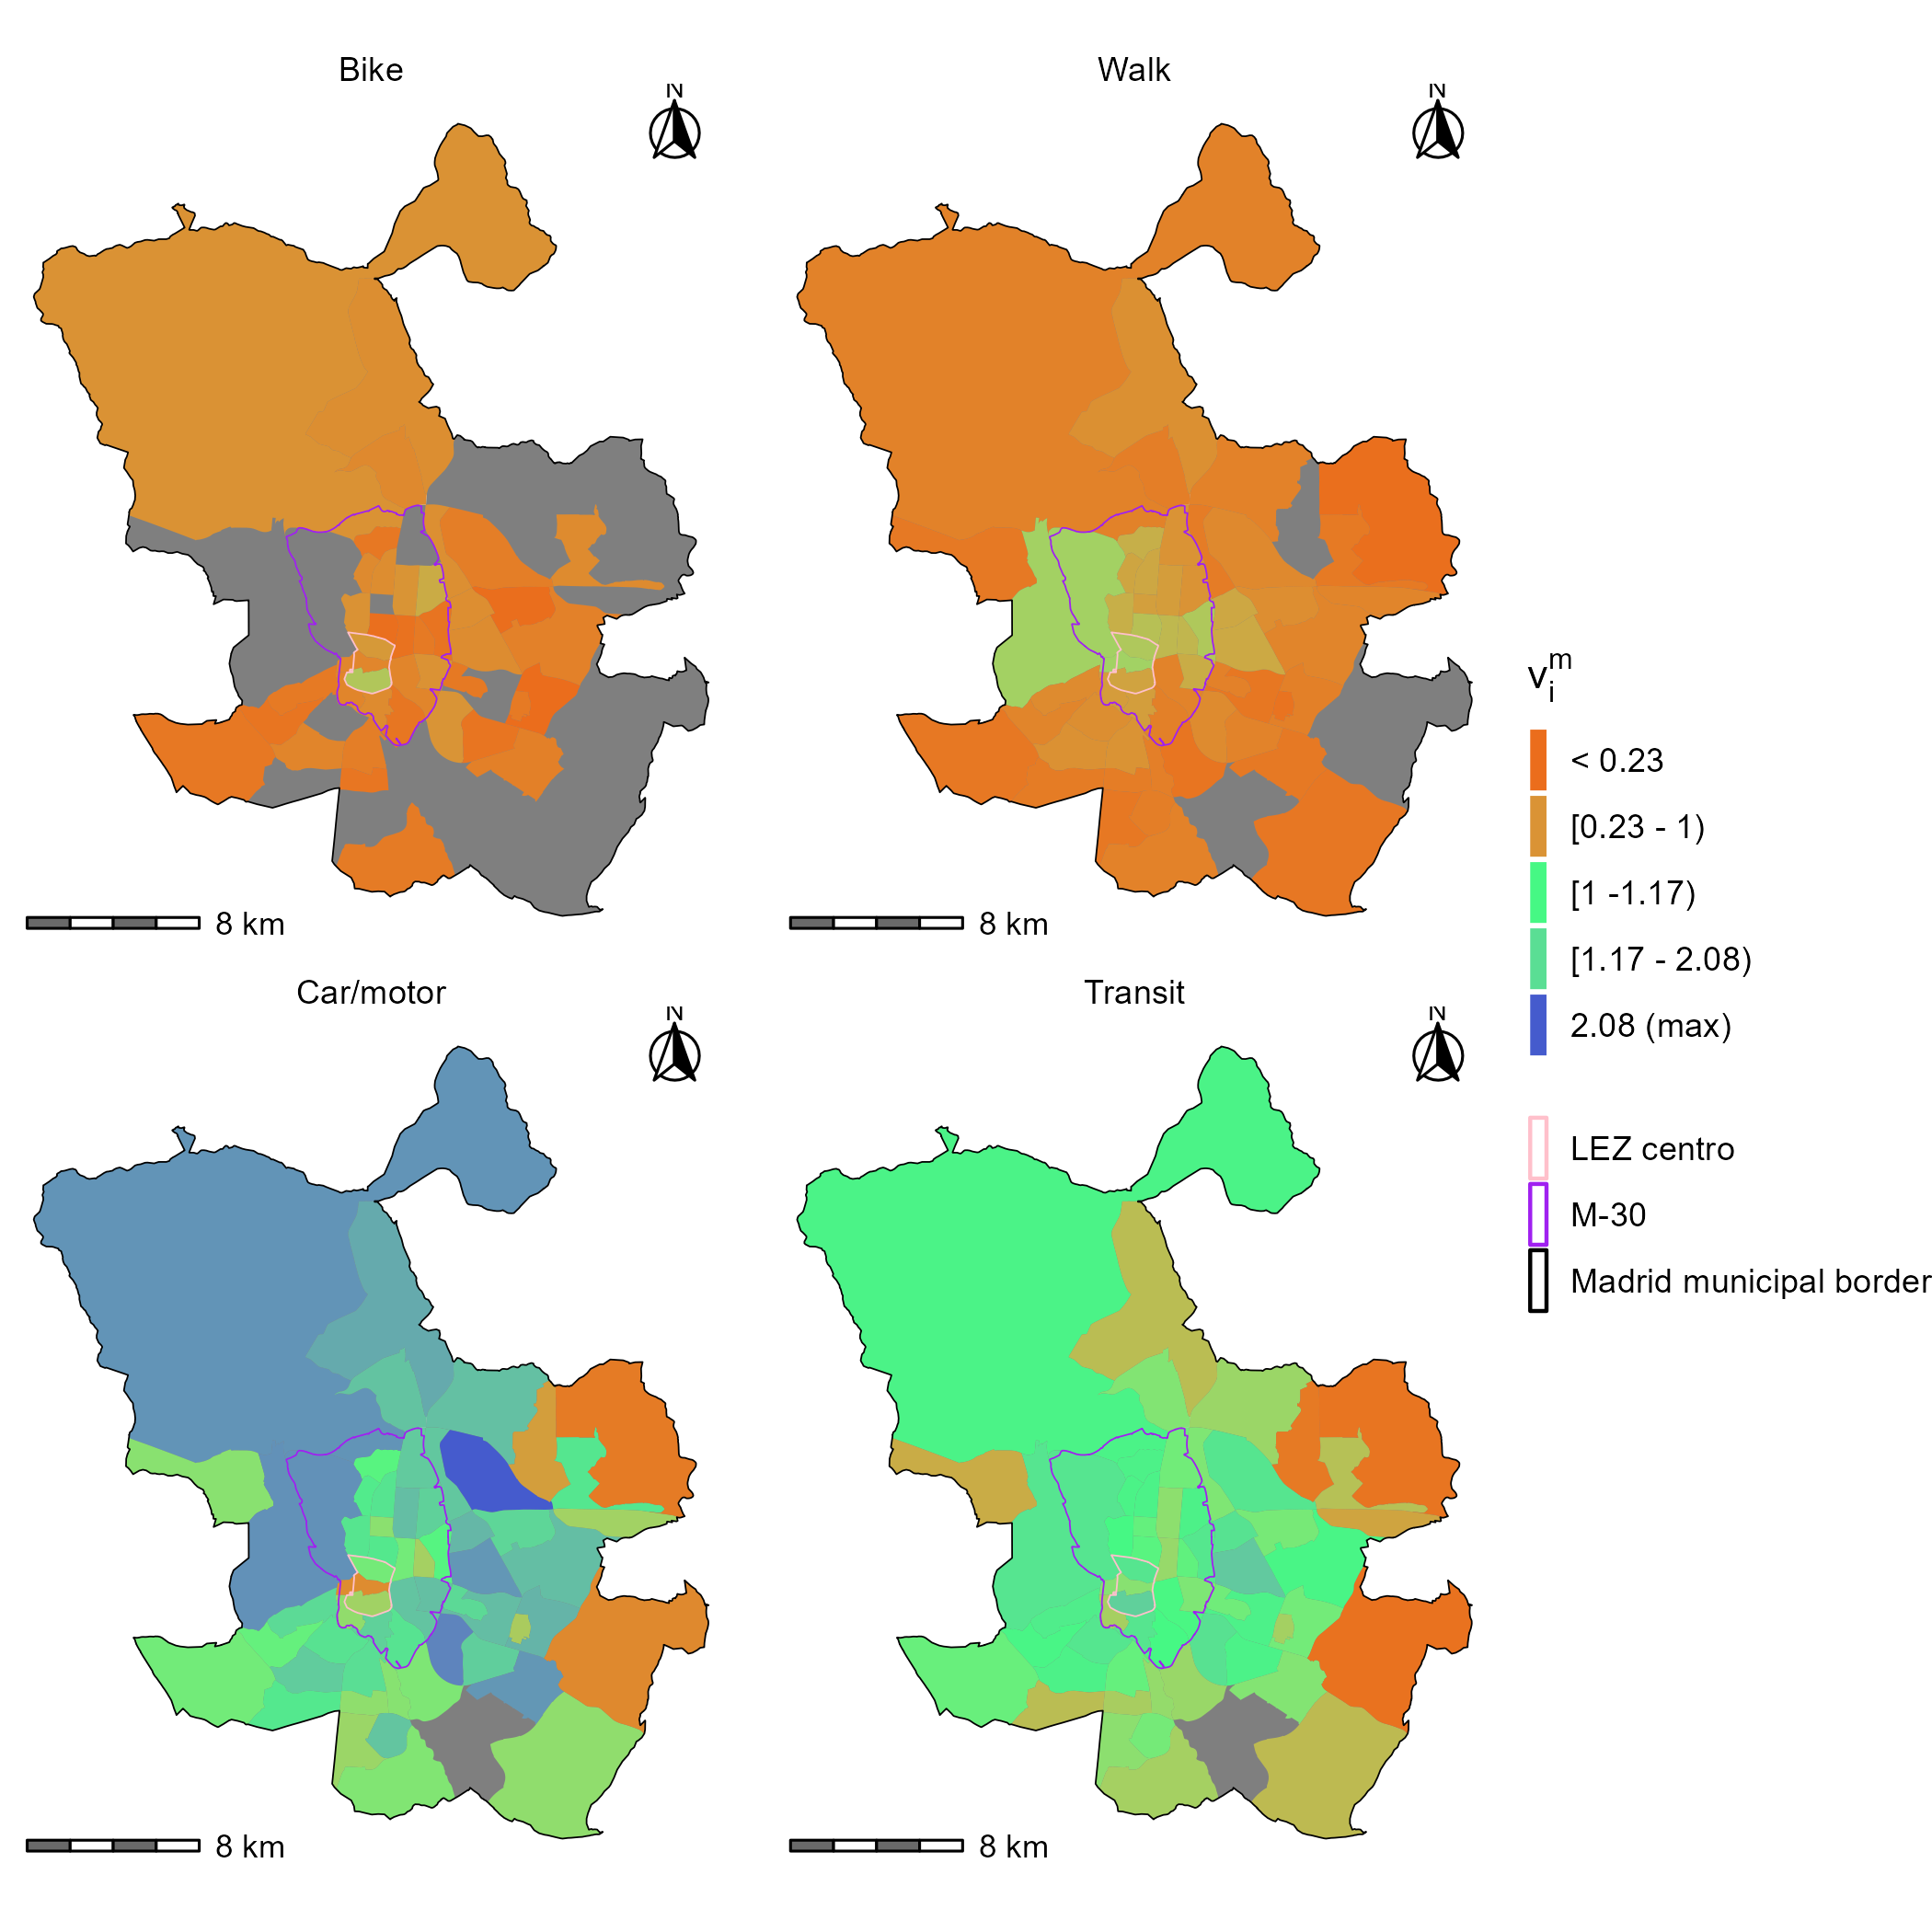
\includegraphics[width=0.85\linewidth]{images/Fig7} 
\DIFaddendFL 

}

\caption{\label{fig:Fig7} \DIFdelbeginFL \DIFdelFL{Spatial availability }\DIFdelendFL \DIFaddbeginFL \DIFaddFL{Distribution }\DIFaddendFL of \DIFdelbeginFL \DIFdelFL{job opportunities }\DIFdelendFL \DIFaddbeginFL \DIFaddFL{spatially available jobs }\DIFaddendFL per \DIFdelbeginFL \DIFdelFL{mode-using }\DIFdelendFL capita by mode \DIFaddbeginFL \DIFaddFL{of transportatin (}\DIFaddendFL $v_i^m$\DIFdelbeginFL \DIFdelFL{per origin in Madrid}\DIFdelendFL \DIFaddbeginFL \DIFaddFL{)}\DIFaddendFL . \DIFdelbeginFL \DIFdelFL{Calculated using }\DIFdelendFL \DIFaddbeginFL \DIFaddFL{Grey TAZs have no population that use }\DIFaddendFL the \DIFdelbeginFL \DIFdelFL{home-to-work origin destination flows from }\DIFdelendFL \DIFaddbeginFL \DIFaddFL{mode. Ranges of values in }\DIFaddendFL the \DIFdelbeginFL \DIFdelFL{2018 travel survey}\DIFdelendFL \DIFaddbeginFL \DIFaddFL{legend are quintiles}\DIFaddendFL .}\label{fig:SA-per-capita-m-plot}
\end{figure}

\DIFdelbegin \DIFdel{Interestingly, as also represented in Figure \ref{fig:Fig6}, }\DIFdelend \DIFaddbegin \DIFadd{Incidentally, }\DIFaddend \(v_i^m\) \DIFdelbegin \DIFdel{for car/motor }\DIFdelend \DIFaddbegin \DIFadd{values for car }\DIFaddend within and near \DIFdelbegin \DIFdel{the }\DIFdelend LEZ Centro is
\DIFdelbegin \DIFdel{near or below 1
(white/red) }\DIFdelend \DIFaddbegin \DIFadd{close to or below one }\DIFaddend in Figure \ref{fig:Fig7}\DIFaddbegin \DIFadd{, }\DIFaddend while all non-car modes
have relatively higher \(v_i^m\) values. \DIFdelbegin \DIFdel{Though the spatial availability from
before the LEZ Centro implementation is unknown}\DIFdelend \DIFaddbegin \DIFadd{Since these values are
comparable across regions and over time}\DIFaddend , Figure \ref{fig:Fig7}
\DIFaddbegin \DIFadd{potentially }\DIFaddend provides a benchmark for quantifying \DIFdelbegin \DIFdel{potential LEZ implementations }\DIFdelend \DIFaddbegin \DIFadd{changes in LEZ policies
}\DIFaddend in the future\DIFdelbegin \DIFdel{(given 2018 travel conditions). }\DIFdelend \DIFaddbegin \DIFadd{. As }\DIFaddend Figure \ref{fig:Fig7} also shows\DIFdelbegin \DIFdel{that }\DIFdelend \DIFaddbegin \DIFadd{, }\DIFaddend many areas within
the M-30 have high (white/green) \(v_i^m\) values for \DIFdelbegin \DIFdel{car-mode, signaling that the
}\DIFdelend \DIFaddbegin \DIFadd{car, but the
results for LEZ Centro give reasonable grounds to speculate that a
}\DIFaddend spatial expansion of the LEZ \DIFdelbegin \DIFdel{Centro stands to }\DIFdelend \DIFaddbegin \DIFadd{to include all areas within the M-30 would
likely }\DIFaddend increase the spatial availability of jobs for \DIFdelbegin \DIFdel{non-car
mode using populations}\DIFdelend \DIFaddbegin \DIFadd{transit users,
cyclists and pedestrians}\DIFaddend .

\hypertarget{discussion-and-conclusions}{%
\section{Discussion and conclusions}\label{discussion-and-conclusions}}

\DIFdelbegin \DIFdel{Location-based accessibility measures like the }\DIFdelend \DIFaddbegin \DIFadd{Accessibility measures are an important tool in transportation research
}{[}\DIFadd{9}{]} \DIFadd{and are increasingly seen as valuable for planning purposes
}{[}\DIFadd{4--8}{]}\DIFadd{. They boast a long history of development, beginning with
}\DIFaddend Hansen-type \(S_i^m\) \DIFdelbegin \DIFdel{,
Shen-type }\DIFdelend \DIFaddbegin \DIFadd{measures, with other developments like Shen's
}\DIFaddend \(a_i^m\), \DIFdelbegin \DIFdel{and spatial availability }\DIFdelend \DIFaddbegin \DIFadd{to account for competition/congestion. The more recent
spatial availability measure }\DIFaddend \(V_i^m\) \DIFdelbegin \DIFdel{measures share a commonality; they are a }\DIFdelend \DIFaddbegin \DIFadd{has in common with these
accessibility indicators that it is a }\DIFaddend weighted sum of \DIFdelbegin \DIFdel{opportunities assigned to each
spatial unit \(i\) }\DIFdelend \DIFaddbegin \DIFadd{the opportunities
}\DIFaddend in a region \DIFdelbegin \DIFdel{. }\DIFdelend \DIFaddbegin \DIFadd{from the perspective of a determined origin \(i\).
Aggregations of opportunities embody principles of gravitational/spatial
interaction modelling that date back to at least H.C. Carey }{[}\DIFadd{49}{]}\DIFadd{,
and are part of a line of research that includes the work of Ravenstein
}{[}\DIFadd{50}{]}\DIFadd{, Reilly }{[}\DIFadd{51}{]}\DIFadd{, Stewart }{[}\DIFadd{52--54}{]}\DIFadd{, Zipf }{[}\DIFadd{55,56}{]}\DIFadd{,
Wilson }{[}\DIFadd{37}{]}\DIFadd{, and many others. }\DIFaddend In this way, \DIFdelbegin \DIFdel{they all }\DIFdelend \DIFaddbegin \DIFadd{\(S_i^m\), \(a_i^m\), and
yes, \(V_i^m\), }\DIFaddend can be interpreted as \DIFdelbegin \DIFdel{a score of how many opportunities can be potentially interacted with
by the population at \(i\).
How the weight
and sum of the
potentially-interacted-with opportunitiesis considered is what defines
the type of accessibility measure.
}\DIFdelend \DIFaddbegin \DIFadd{scores of the potential for
interaction with opportunities in space.
}\DIFaddend 

\DIFdelbegin \DIFdel{Within this paper, the location-based singly- }\emph{\DIFdel{constrained}} %DIFAUXCMD
\DIFdel{and
}\emph{\DIFdel{competitive}} %DIFAUXCMD
\DIFdel{accessibility measure
, known as spatial availability \(V_i\) }\DIFdelend \DIFaddbegin \DIFadd{Different accessibility indicators are characterized by how they weight
and aggregate opportunities. Spatial availability's contribution to the
literature is to incorporate a proportional allocation mechanism that
essentially constrains the sums to match the number of opportunities in
the region; in this way it is a singly-constrained accessibility measure
that naturally accommodates congestion and competition. The effort with
spatial availability is in line with previous research on proportional
allocation by Paez et al. }\DIFaddend {[}14{]}\DIFdelbegin \DIFdel{, is extended }\DIFdelend \DIFaddbegin \DIFadd{. As initially introduced by Soukhov
et al. }{[}\DIFadd{15}{]}\DIFadd{, spatial availability was designed for a homogeneous
population traveling by a single mode of transportation. In this paper,
we extended spatial availability }\DIFaddend for the case of \DIFdelbegin \DIFdel{capturing multimodal
accessibility to opportunities \(V_i^m\). A synthetic example and then
an empirical case of LEZ in Madrid are detailed to demonstrate this
multimodal extension.
}\DIFdelend \DIFaddbegin \DIFadd{heterogeneous
populations. We discussed this in terms of multiple modes of
transportation, but the framework can accommodate equally well
variations in travel behavior by population segments.
}\DIFaddend 

\DIFdelbegin \DIFdel{The spatial availability measure is capable of capturing a new
interpretation of multimodal competition that previous accessibility
measures have not yet done. Competitive measures hypothesis that
populations using modes with lower travel impedance, when competing for a finite set of opportunities , will capture more opportunities. With
spatial availability
, the }\DIFdelend \DIFaddbegin \DIFadd{An empirical example using data from Madrid helped to illustrate the
potential of multimodal spatial availability analysis, including its
ability to account for competition for opportunities within and between
modes. Particularly relevant is the fact that spatial availability
scores relate directly to the total }\DIFaddend number of opportunities \DIFdelbegin \DIFdel{that are captured (of
the total opportunities }\DIFdelend in the
region\DIFdelbegin \DIFdel{) by each mode can be individually
calculated. From there, the difference between how many spatially
available opportunities one mode captures versus another can be
investigated. This is the advantage of the spatial availability measure, particularly its multimodal extension.
}%DIFDELCMD < 

%DIFDELCMD < %%%
\DIFdel{The flexibility and need for an accessibility measure such as spatial
availability is pertinent in policy scenario evaluation. As showcased in
the empirical example of the LEZ in Madrid, competition for job
opportunity availability varies spatially }\emph{\DIFdel{as well as}} %DIFAUXCMD
\DIFdel{between modes. The car and transit modes have the highest spatial availability, with the car-mode having highest availability with exception to
the
areas within the LEZ Centro. Since car travel has been highly restricted
within the LEZ Centro, fewer car-using people potentially interact with
jobs within the LEZ Centro, leaving more }\emph{\DIFdel{spatially available}} %DIFAUXCMD
\DIFdel{jobs
for
non-car-using populations}\DIFdelend . This \DIFaddbegin \DIFadd{makes it possible to compare the results to intuitive
benchmarks, such as opportunities per population, in ways that other
accessibility measures cannot or tend to obfuscate. This comparability
is preserved between regions and over time. The example suggests that
once that opportunities are treated as being finite, restrictions to
travel by car leave more spatially available opportunities for
non-car-users. This }\DIFaddend difference \DIFdelbegin \DIFdel{in car-using populations
in locations accessing jobs }\DIFdelend \DIFaddbegin \DIFadd{for car travel in locations }\DIFaddend within and
immediately \DIFdelbegin \DIFdel{outside }\DIFdelend \DIFaddbegin \DIFadd{around }\DIFaddend the LEZ Centro \DIFdelbegin \DIFdel{increases the competitiveness of
}\DIFdelend \DIFaddbegin \DIFadd{seems to increase the number of
opportunities spatially available to transit users (transit being }\DIFaddend the
\DIFdelbegin \DIFdel{transit-using population
(the }\DIFdelend second most competitive mode)\DIFaddbegin \DIFadd{, }\DIFaddend as well as the \DIFaddbegin \DIFadd{spatial availability from
the perspective of }\DIFaddend non-motorized modes. \DIFaddbegin \DIFadd{In effect, a policy such as Low
Emission Zones help to improve the accessibility situation of active
travel and transit in the parts of the city where it is implemented.
}\DIFaddend 

\DIFdelbegin \DIFdel{Spatial availability \(V_i^m\) can also be divided by the mode-using
population at each \(i\) to yield mode-population normalized values. These values, reflected in Figure \ref{fig:Fig7}, can be used as a
benchmark to
investigate existing conditions and plan future LEZ implementation (i.e., target areas with exceptionally high car spatial
availability such that more opportunities are available to other
mode-users).
}\DIFdelend \DIFaddbegin \DIFadd{The purpose of the empirical example is to illustrate the kind of
insights that can be derived from the application of multimodal spatial
availability. But there are some intriguing opportunities for future
research. Accessibility indicators are not designed to work as modal
split models, and yet, in the case of policies that alter the relative
cost of various forms of transportation, one can reasonably expect to
see some shifts between modes. In our empirical example we used data
collected }\emph{\DIFadd{after}} \DIFadd{the introduction of LEZ Centro. However, given a
modal split model to project model shares, accessibility indicators,
including spatial availability, can be used to investigate changes to
the accessibility landscape. Ditto for destination choice. Our empirical
example presented but a snapshot of this, and in future research it will
be interesting to investigate changes }\emph{\DIFadd{between}} \DIFadd{policy
interventions. The expansion of Madrid's LEZ to the ring contained by
the M-30 orbital presents an excellent opportunity to do so. Given the
intuitive and straightforward interpretation of spatial availability
scores as fractions of opportunities from the total, relative and
absolute changes in the accessibility landscape can be assessed, thus
helping to evaluate the implications of policy interventions.
}\DIFaddend 

\DIFdelbegin \DIFdel{In summary, conventional }\emph{\DIFdel{non-constrained}} %DIFAUXCMD
\DIFdel{accessibility measures
are difficult for planners to operationalize for a variety of reasons
including issues of computation and interpretability }\DIFdelend \DIFaddbegin \DIFadd{Finally, our example dealt with differences in travel by mode only, but
it is possible to think of the intersection between mode of travel and
different types of travelers. This would expand the number of
sub-populations in the analysis from, say, \(m=M\) (modes) to
\(m = M\cdot Q\) (modes times population segments), each with their own
characteristic impedance function. Evaluations of this kind will be
especially relevant as LEZ are implemented in cities globally, and the
question of their impact on disadvantaged populations who have become
mobility-restricted increasingly come to the fore }\DIFaddend {[}\DIFdelbegin \DIFdel{2}\DIFdelend \DIFaddbegin \DIFadd{40,57,58}\DIFaddend {]}\DIFdelbegin \DIFdel{. With
spatial availability, the magnitude of opportunities that are available
as a proportion of all the opportunities in the region is equal to \(V_i\). As a result of its proportional allocation mechanism, \(V_i\)
can be naturally extended into multimodal applications. This flexibility
is helpful to modelling policy
scenarios in our cities that are
increasingly multimodal. The interpretation of \(V_i\) allows for
manipulation of \(V_i^m\) values to investigate differences of availability between neighbourhoods, modes, and
regions, generate per
capita benchmarks, and/or generate average values per population-group}\DIFdelend .

\DIFdelbegin \DIFdel{From a spatial equity perspective, spatial availability measure can
provide researchers, policy makers, and
citizens a new-found
interpretation of accessibility measures. With a plot of
spatial
availability values, one can begin asking, how much is enough and what
level may be too much. These interpretations were difficult to
be made
with accessibility measures in the past.
}%DIFDELCMD < 

%DIFDELCMD < %%%
\DIFdelend \hypertarget{acknowledgements}{%
\section{Acknowledgements}\label{acknowledgements}}

This research was funded by the Canada Graduate Scholarship - Doctoral
Program (CGS D) provided by the Social Sciences and Humanities Research
Council (SSHRC) and Project Mobilizing Justice, also supported by SSHRC.
The funders had no role in study design, data collection and analysis,
decision to publish, or preparation of the manuscript.

All work is fully-reproducible and available within this
\href{https://github.com/soukhova/Multimodal-spatial-availability}{GitHub
repository}.

\hypertarget{author-contributions}{%
\section{Author contributions}\label{author-contributions}}

The authors confirm contribution to the paper as follows: study
conception and design: AS, JTO, JSL, AP.; data collection: AS, JTO,
JSL.; analysis and interpretation of results: AS, JTO, JSL, AP.; draft
manuscript preparation: AS, JSL, AP. All authors reviewed the results
and approved the final version of the manuscript.

\hypertarget{references}{%
\section*{References}\label{references}}
\addcontentsline{toc}{section}{References}

\hypertarget{refs}{}
\begin{CSLReferences}{0}{0}
\leavevmode\vadjust pre{\hypertarget{ref-hansenHowAccessibilityShapes1959}{}}%
\CSLLeftMargin{1. }%
\CSLRightInline{Hansen WG. How accessibility shapes land use. Journal of
the American Institute of Planners. 1959;25: 73--76.
doi:\href{https://doi.org/10.1080/01944365908978307}{10.1080/01944365908978307}}

\leavevmode\vadjust pre{\DIFdelbegin %DIFDELCMD < \hypertarget{ref-levinsonTransportAccessManual2020}{}%%%
\DIFdelend \DIFaddbegin \hypertarget{ref-geursAccessibility2004}{}\DIFaddend }%
\CSLLeftMargin{2. }%
\DIFdelbegin %DIFDELCMD < \CSLRightInline{Levinson D, King D. Transport access manual: {A} guide
%DIFDELCMD < for measuring connection between people and places. {University of
%DIFDELCMD < Sydney}; 2020. Available:
%DIFDELCMD < \url{https://ses.library.usyd.edu.au/handle/2123/23733}}
%DIFDELCMD < %%%
\DIFdelend \DIFaddbegin \CSLRightInline{Geurs KT, Wee B van. Accessibility evaluation of
land-use and transport strategies: Review and research directions.
Journal of Transport Geography. 2004;12: 127--140. Available:
\href{http://www.sciencedirect.com/science/article/B6VG8-4B28VY7-1/2/61478339c14cab4fa58438ad7b1f4610\%0AC:/Papers/Journal\%20of\%20Transport\%20Geography/Journal\%20of\%20Transport\%20Geography\%20(2004)\%2012\%20(2)\%20127-140.pdf}{http://www.sciencedirect.com/science/article/B6VG8-4B28VY7-1/2/61478339c14cab4fa58438ad7b1f4610
C:/Papers/Journal of Transport Geography/Journal of Transport Geography
(2004) 12 (2) 127-140.pdf}}
\DIFaddend 

\leavevmode\vadjust pre{\DIFdelbegin %DIFDELCMD < \hypertarget{ref-gowerPlanningInnovationCity2022}{}%%%
\DIFdelend \DIFaddbegin \hypertarget{ref-paezPositive2012}{}\DIFaddend }%
\CSLLeftMargin{3. }%
\DIFdelbegin %DIFDELCMD < \CSLRightInline{Gower A, Grodach C. Planning innovation or city
%DIFDELCMD < branding? Exploring how cities operationalise the 20-minute
%DIFDELCMD < neighbourhood concept. Urban Policy and Research. 2022;40: 36--52.
%DIFDELCMD < doi:\href{https://doi.org/10.1080/08111146.2021.2019701}{10.1080/08111146.2021.2019701}}
%DIFDELCMD < %%%
\DIFdelend \DIFaddbegin \CSLRightInline{Paez A, Scott DM, Morency C. Measuring accessibility:
Positive and normative implementations of various accessibility
indicators. Journal of Transport Geography. 2012;25: 141--153.
doi:\href{https://doi.org/10.1016/j.jtrangeo.2012.03.016}{10.1016/j.jtrangeo.2012.03.016}}
\DIFaddend 

\leavevmode\vadjust pre{\DIFdelbegin %DIFDELCMD < \hypertarget{ref-siddiqToolsTradeAssessing2021}{}%%%
\DIFdelend \DIFaddbegin \hypertarget{ref-handyAccessibility2020}{}\DIFaddend }%
\CSLLeftMargin{4. }%
\DIFdelbegin %DIFDELCMD < \CSLRightInline{Siddiq F, D. Taylor B. Tools of the trade?: Assessing
%DIFDELCMD < the progress of accessibility measures for planning practice. Journal of
%DIFDELCMD < the American Planning Association. 2021;87: 497--511.
%DIFDELCMD < doi:\href{https://doi.org/10.1080/01944363.2021.1899036}{10.1080/01944363.2021.1899036}}
%DIFDELCMD < %%%
\DIFdelend \DIFaddbegin \CSLRightInline{Handy S. Is accessibility an idea whose time has finally
come? Transportation Research Part D: Transport and Environment.
2020;83: 102319. doi:\url{https://doi.org/10.1016/j.trd.2020.102319}}
\DIFaddend 

\leavevmode\vadjust pre{\DIFdelbegin %DIFDELCMD < \hypertarget{ref-yanAccessibilityBasedPlanningAddressing2021}{}%%%
\DIFdelend \DIFaddbegin \hypertarget{ref-levinsonTransportAccessManual2020}{}\DIFaddend }%
\CSLLeftMargin{5. }%
\DIFdelbegin %DIFDELCMD < \CSLRightInline{Yan X. Toward accessibility-based planning addressing
%DIFDELCMD < the myth of travel cost savings. {JOURNAL} {OF} {THE} {AMERICAN}
%DIFDELCMD < {PLANNING} {ASSOCIATION}. 2021;87: 409--423.
%DIFDELCMD < doi:\href{https://doi.org/10.1080/01944363.2020.1850321}{10.1080/01944363.2020.1850321}}
%DIFDELCMD < %%%
\DIFdelend \DIFaddbegin \CSLRightInline{Levinson D, King D. Transport access manual: {A} guide
for measuring connection between people and places. {University of
Sydney}; 2020. Available:
\url{https://ses.library.usyd.edu.au/handle/2123/23733}}
\DIFaddend 

\leavevmode\vadjust pre{\DIFdelbegin %DIFDELCMD < \hypertarget{ref-fikselSustainabilityResilienceSystems2006}{}%%%
\DIFdelend \DIFaddbegin \hypertarget{ref-siddiqToolsTradeAssessing2021}{}\DIFaddend }%
\CSLLeftMargin{6. }%
\DIFdelbegin %DIFDELCMD < \CSLRightInline{Fiksel J. Sustainability and resilience: Toward a
%DIFDELCMD < systems approach. Sustainability: Science, Practice and Policy. 2006;2:
%DIFDELCMD < 14--21.
%DIFDELCMD < doi:\href{https://doi.org/10.1080/15487733.2006.11907980}{10.1080/15487733.2006.11907980}}
%DIFDELCMD < %%%
\DIFdelend \DIFaddbegin \CSLRightInline{Siddiq F, D. Taylor B. Tools of the trade?: Assessing
the progress of accessibility measures for planning practice. Journal of
the American Planning Association. 2021;87: 497--511.
doi:\href{https://doi.org/10.1080/01944363.2021.1899036}{10.1080/01944363.2021.1899036}}
\DIFaddend 

\leavevmode\vadjust pre{\DIFdelbegin %DIFDELCMD < \hypertarget{ref-valencaMainChallengesOpportunities2021}{}%%%
\DIFdelend \DIFaddbegin \hypertarget{ref-yanAccessibilityBasedPlanningAddressing2021}{}\DIFaddend }%
\CSLLeftMargin{7. }%
\DIFdelbegin %DIFDELCMD < \CSLRightInline{Valença G, Moura F, Morais De Sá A. Main challenges and
%DIFDELCMD < opportunities to dynamic road space allocation: From static to dynamic
%DIFDELCMD < urban designs. Journal of Urban Mobility. 2021;1: 100008.
%DIFDELCMD < doi:\href{https://doi.org/10.1016/j.urbmob.2021.100008}{10.1016/j.urbmob.2021.100008}}
%DIFDELCMD < %%%
\DIFdelend \DIFaddbegin \CSLRightInline{Yan X. Toward accessibility-based planning addressing
the myth of travel cost savings. {JOURNAL} {OF} {THE} {AMERICAN}
{PLANNING} {ASSOCIATION}. 2021;87: 409--423.
doi:\href{https://doi.org/10.1080/01944363.2020.1850321}{10.1080/01944363.2020.1850321}}
\DIFaddend 

\leavevmode\vadjust pre{\DIFdelbegin %DIFDELCMD < \hypertarget{ref-leeMeasuringImpactsNew2018}{}%%%
\DIFdelend \DIFaddbegin \hypertarget{ref-elGeneidyMaking2022}{}\DIFaddend }%
\CSLLeftMargin{8. }%
\DIFdelbegin %DIFDELCMD < \CSLRightInline{Lee J, Miller HJ. Measuring the impacts of new public
%DIFDELCMD < transit services on space-time accessibility: An analysis of transit
%DIFDELCMD < system redesign and new bus rapid transit in columbus, ohio, {USA}.
%DIFDELCMD < Applied Geography. 2018;93: 47--63.
%DIFDELCMD < doi:\href{https://doi.org/10.1016/j.apgeog.2018.02.012}{10.1016/j.apgeog.2018.02.012}}
%DIFDELCMD < %%%
\DIFdelend \DIFaddbegin \CSLRightInline{El-Geneidy A, Levinson D. Making accessibility work in
practice. Transport Reviews. 2022;42: 129--133.
doi:\href{https://doi.org/10.1080/01441647.2021.1975954}{10.1080/01441647.2021.1975954}}
\DIFaddend 

\leavevmode\vadjust pre{\DIFdelbegin %DIFDELCMD < \hypertarget{ref-mohriClusteringMethodMeasuring2021}{}%%%
\DIFdelend \DIFaddbegin \hypertarget{ref-shiLiterature2020}{}\DIFaddend }%
\CSLLeftMargin{9. }%
\DIFdelbegin %DIFDELCMD < \CSLRightInline{Mohri S, Mortazavi S, Nassir N. A clustering method for
%DIFDELCMD < measuring accessibility and equity in public transportation service:
%DIFDELCMD < {Case} study of {Melbourne}. SUSTAINABLE CITIES AND SOCIETY. 2021;74.
%DIFDELCMD < doi:\href{https://doi.org/10.1016/j.scs.2021.103241}{10.1016/j.scs.2021.103241}}
%DIFDELCMD < %%%
\DIFdelend \DIFaddbegin \CSLRightInline{Shi Y, Blainey S, Sun C, Jing P. A literature review on
accessibility using bibliometric analysis techniques. Journal of
Transport Geography. 2020;87: 102810.
doi:\href{https://doi.org/10.1016/j.jtrangeo.2020.102810}{10.1016/j.jtrangeo.2020.102810}}
\DIFaddend 

\leavevmode\vadjust pre{\DIFdelbegin %DIFDELCMD < \hypertarget{ref-maoMeasuringSpatialAccessibility2013}{}%%%
\DIFdelend \DIFaddbegin \hypertarget{ref-handyMeasuring1997}{}\DIFaddend }%
\CSLLeftMargin{10. }%
\DIFdelbegin %DIFDELCMD < \CSLRightInline{Mao L, Nekorchuk D. Measuring spatial accessibility to
%DIFDELCMD < healthcare for populations with multiple transportation modes. Health \&
%DIFDELCMD < Place. 2013;24: 115--122.
%DIFDELCMD < doi:\href{https://doi.org/10.1016/j.healthplace.2013.08.008}{10.1016/j.healthplace.2013.08.008}}
%DIFDELCMD < %%%
\DIFdelend \DIFaddbegin \CSLRightInline{Handy S, Niemeier D. Measuring accessibility: An
exploration of issues and alternatives. Environment and Planning A.
1997;29: 1175--1194. }
\DIFaddend 

\leavevmode\vadjust pre{\DIFdelbegin %DIFDELCMD < \hypertarget{ref-tarrinoortizPublicAcceptabilityLow2021}{}%%%
\DIFdelend \DIFaddbegin \hypertarget{ref-kwanSpace1998}{}\DIFaddend }%
\CSLLeftMargin{11. }%
\DIFdelbegin %DIFDELCMD < \CSLRightInline{Tarriño-Ortiz J, Soria-Lara JA, Gómez J, Vassallo JM.
%DIFDELCMD < Public acceptability of low emission zones: The case of {``madrid
%DIFDELCMD < central.''} Sustainability. 2021;13: 3251.
%DIFDELCMD < doi:\href{https://doi.org/10.3390/su13063251}{10.3390/su13063251}}
%DIFDELCMD < %%%
\DIFdelend \DIFaddbegin \CSLRightInline{Kwan MP. Space-time and integral measures of individual
accessibility: A comparative analysis using a point-based framework.
Geographical Analysis. 1998;30: 191--216. Available:
\href{https://ISI:000074579200001\%0AC:/Papers/Geographical\%20Analysis/Geographical\%20Analysis\%20(1998)\%2030\%20(3)\%20191-216.pdf}{ISI:000074579200001
C:/Papers/Geographical Analysis/Geographical Analysis (1998) 30 (3)
191-216.pdf}}
\DIFaddend 

\leavevmode\vadjust pre{\DIFdelbegin %DIFDELCMD < \hypertarget{ref-devrijNooneVisitsMe2022}{}%%%
\DIFdelend \DIFaddbegin \hypertarget{ref-shenLocationCharacteristicsInnercity1998}{}\DIFaddend }%
\CSLLeftMargin{12. }%
\DIFdelbegin %DIFDELCMD < \CSLRightInline{De Vrij E, Vanoutrive T. {``No-one visits me anymore''}:
%DIFDELCMD < Low emission zones and social exclusion via sustainable transport
%DIFDELCMD < policy. 2022 {[}cited 27 Jul 2023{]}. Available:
%DIFDELCMD < \url{https://www.tandfonline.com/doi/epdf/10.1080/1523908X.2021.2022465?needAccess=true\&role=button}}
%DIFDELCMD < %%%
\DIFdelend \DIFaddbegin \CSLRightInline{Shen Q. Location characteristics of inner-city
neighborhoods and employment accessibility of low-wage workers. Environ
Plann B. 1998;25: 345--365.
doi:\href{https://doi.org/10.1068/b250345}{10.1068/b250345}}
\DIFaddend 

\leavevmode\vadjust pre{\DIFdelbegin %DIFDELCMD < \hypertarget{ref-verbeekJustManagementUrban2022}{}%%%
\DIFdelend \DIFaddbegin \hypertarget{ref-luoMeasuresSpatialAccessibility2003}{}\DIFaddend }%
\CSLLeftMargin{13. }%
\DIFdelbegin %DIFDELCMD < \CSLRightInline{Verbeek T, Hincks S. The {``just''} management of urban
%DIFDELCMD < air pollution? A geospatial analysis of low emission zones in brussels
%DIFDELCMD < and london. Applied Geography. 2022;140: 102642.
%DIFDELCMD < doi:\href{https://doi.org/10.1016/j.apgeog.2022.102642}{10.1016/j.apgeog.2022.102642}}
%DIFDELCMD < %%%
\DIFdelend \DIFaddbegin \CSLRightInline{Luo W, Wang F. Measures of spatial accessibility to
health care in a {GIS} environment: Synthesis and a case study in the
chicago region. Environ Plann B Plann Des. 2003;30: 865--884.
doi:\href{https://doi.org/10.1068/b29120}{10.1068/b29120}}
\DIFaddend 

\leavevmode\vadjust pre{\DIFdelbegin %DIFDELCMD < \hypertarget{ref-soukhovIntroducingSpatialAvailability2023}{}%%%
\DIFdelend \DIFaddbegin \hypertarget{ref-paezDemand2019}{}\DIFaddend }%
\CSLLeftMargin{14. }%
\DIFdelbegin %DIFDELCMD < \CSLRightInline{Soukhov A, Paez A, Higgins CD, Mohamed M. Introducing
%DIFDELCMD < spatial availability, a singly-constrained measure of competitive
%DIFDELCMD < accessibility {\textbar} {PLOS} {ONE}. {PLOS} {ONE}. 2023; 1--30.
%DIFDELCMD < doi:\href{https://\%20doi.org/10.1371/journal.pone.0278468}{https://
%DIFDELCMD < doi.org/10.1371/journal.pone.0278468}}
%DIFDELCMD < %%%
\DIFdelend \DIFaddbegin \CSLRightInline{Paez A, Higgins CD, Vivona SF. Demand and level of
service inflation in floating catchment area (FCA) methods. PloS one.
2019;14: e0218773.
doi:\href{https://doi.org/10.1371/journal.pone.0218773}{10.1371/journal.pone.0218773}}
\DIFaddend 

\leavevmode\vadjust pre{\DIFdelbegin %DIFDELCMD < \hypertarget{ref-tahmasbiMultimodalAccessibilitybasedEquity2019}{}%%%
\DIFdelend \DIFaddbegin \hypertarget{ref-soukhovIntroducingSpatialAvailability2023}{}\DIFaddend }%
\CSLLeftMargin{15. }%
\DIFdelbegin %DIFDELCMD < \CSLRightInline{Tahmasbi B, Mansourianfar MH, Haghshenas H, Kim I.
%DIFDELCMD < Multimodal accessibility-based equity assessment of urban public
%DIFDELCMD < facilities distribution. Sustainable Cities and Society. 2019;49:
%DIFDELCMD < 101633.
%DIFDELCMD < doi:\href{https://doi.org/10.1016/j.scs.2019.101633}{10.1016/j.scs.2019.101633}}
%DIFDELCMD < %%%
\DIFdelend \DIFaddbegin \CSLRightInline{Soukhov A, Paez A, Higgins CD, Mohamed M. Introducing
spatial availability, a singly-constrained measure of competitive
accessibility \textbar{} {PLOS ONE}. PLOS ONE. 2023; 1--30.
doi:\href{https://\%20doi.org/10.1371/journal.pone.0278468}{https://
doi.org/10.1371/journal.pone.0278468}}
\DIFaddend 

\leavevmode\vadjust pre{\DIFdelbegin %DIFDELCMD < \hypertarget{ref-luoMeasuresSpatialAccessibility2003}{}%%%
\DIFdelend \DIFaddbegin \hypertarget{ref-paezHealth2010}{}\DIFaddend }%
\CSLLeftMargin{16. }%
\DIFdelbegin %DIFDELCMD < \CSLRightInline{Luo W, Wang F. Measures of spatial accessibility to
%DIFDELCMD < health care in a {GIS} environment: Synthesis and a case study in the
%DIFDELCMD < chicago region. Environ Plann B Plann Des. 2003;30: 865--884.
%DIFDELCMD < doi:\href{https://doi.org/10.1068/b29120}{10.1068/b29120}}
%DIFDELCMD < %%%
\DIFdelend \DIFaddbegin \CSLRightInline{Páez A, Mercado R, Farber S, Morency C, Roorda M.
Accessibility to health care facilities in montreal island: An
application of relative accessibility indicators from the perspective of
senior and non-senior residents. International Journal of Health
Geographics. 2010;9: 1--9. }
\DIFaddend 

\leavevmode\vadjust pre{\DIFdelbegin %DIFDELCMD < \hypertarget{ref-shenLocationCharacteristicsInnercity1998}{}%%%
\DIFdelend \DIFaddbegin \hypertarget{ref-moniruzzamanMode2013}{}\DIFaddend }%
\CSLLeftMargin{17. }%
\DIFdelbegin %DIFDELCMD < \CSLRightInline{Shen Q. Location characteristics of inner-city
%DIFDELCMD < neighborhoods and employment accessibility of low-wage workers. Environ
%DIFDELCMD < Plann B. 1998;25: 345--365.
%DIFDELCMD < doi:\href{https://doi.org/10.1068/b250345}{10.1068/b250345}}
%DIFDELCMD < %%%
\DIFdelend \DIFaddbegin \CSLRightInline{Moniruzzaman M, Páez A, Nurul Habib KM, Morency C. Mode
use and trip length of seniors in montreal. Journal of Transport
Geography. 2013;30: 89--99.
doi:\url{http://dx.doi.org/10.1016/j.jtrangeo.2013.03.007}}
\DIFaddend 

\leavevmode\vadjust pre{\DIFdelbegin %DIFDELCMD < \hypertarget{ref-weibullAxiomaticApproachMeasurement1976}{}%%%
\DIFdelend \DIFaddbegin \hypertarget{ref-reyesWalking2014}{}\DIFaddend }%
\CSLLeftMargin{18. }%
\DIFdelbegin %DIFDELCMD < \CSLRightInline{Weibull JW. An axiomatic approach to the measurement of
%DIFDELCMD < accessibility. Regional Science and Urban Economics. 1976;6: 357--379.
%DIFDELCMD < doi:\href{https://doi.org/10.1016/0166-0462(76)90031-4}{10.1016/0166-0462(76)90031-4}}
%DIFDELCMD < %%%
\DIFdelend \DIFaddbegin \CSLRightInline{Reyes M, Paez A, Morency C. Walking accessibility to
urban parks by children: A case study of montreal. Landscape and Urban
Planning. 2014;125: 38--47.
doi:\href{https://doi.org/10.1016/j.landurbplan.2014.02.002}{10.1016/j.landurbplan.2014.02.002}}
\DIFaddend 

\leavevmode\vadjust pre{\DIFdelbegin %DIFDELCMD < \hypertarget{ref-josephMeasuringPotentialPhysical1982}{}%%%
\DIFdelend \DIFaddbegin \hypertarget{ref-paezJobs2013}{}\DIFaddend }%
\CSLLeftMargin{19. }%
\DIFdelbegin %DIFDELCMD < \CSLRightInline{Joseph AE, Bantock PR. Measuring potential physical
%DIFDELCMD < accessibility to general practitioners in rural areas: A method and case
%DIFDELCMD < study. Social Science \& Medicine. 1982;16: 85--90.
%DIFDELCMD < doi:\href{https://doi.org/10.1016/0277-9536(82)90428-2}{10.1016/0277-9536(82)90428-2}}
%DIFDELCMD < %%%
\DIFdelend \DIFaddbegin \CSLRightInline{Páez A, Farber S, Mercado R, Roorda M, Morency C. Jobs
and the single parent: An analysis of accessibility to employment in
toronto. Urban Geography. 2013;34: 815--842.
doi:\href{https://doi.org/10.1080/02723638.2013.778600}{10.1080/02723638.2013.778600}}
\DIFaddend 

\leavevmode\vadjust pre{\DIFdelbegin %DIFDELCMD < \hypertarget{ref-taoInvestigatingImpactsPublic2020a}{}%%%
\DIFdelend \DIFaddbegin \hypertarget{ref-wuUnifyingAccess2020}{}\DIFaddend }%
\CSLLeftMargin{20. }%
\DIFdelbegin %DIFDELCMD < \CSLRightInline{Tao Z, Zhou J, Lin X, Chao H, Li G. Investigating the
%DIFDELCMD < impacts of public transport on job accessibility in {Shenzhen}, {China}:
%DIFDELCMD < A multi-modal approach. Land Use Policy. 2020;99: 105025.
%DIFDELCMD < doi:\href{https://doi.org/10.1016/j.landusepol.2020.105025}{10.1016/j.landusepol.2020.105025}}
%DIFDELCMD < %%%
\DIFdelend \DIFaddbegin \CSLRightInline{Wu H, Levinson D. Unifying access. Transportation
Research Part D: Transport and Environment. 2020;83: 102355.
doi:\href{https://doi.org/10.1016/j.trd.2020.102355}{10.1016/j.trd.2020.102355}}
\DIFaddend 

\leavevmode\vadjust pre{\DIFdelbegin %DIFDELCMD < \hypertarget{ref-carpentieriMultimodalAccessibilityPrimary2020}{}%%%
\DIFdelend \DIFaddbegin \hypertarget{ref-tahmasbiMultimodalAccessibilitybasedEquity2019}{}\DIFaddend }%
\CSLLeftMargin{21. }%
\DIFdelbegin %DIFDELCMD < \CSLRightInline{Carpentieri G, Guida C, Masoumi HE. Multimodal
%DIFDELCMD < {Accessibility} to {Primary Health Services} for the {Elderly}: {A Case
%DIFDELCMD < Study} of {Naples}, {Italy}. Sustainability. 2020;12: 781.
%DIFDELCMD < doi:\href{https://doi.org/10.3390/su12030781}{10.3390/su12030781}}
%DIFDELCMD < %%%
\DIFdelend \DIFaddbegin \CSLRightInline{Tahmasbi B, Mansourianfar MH, Haghshenas H, Kim I.
Multimodal accessibility-based equity assessment of urban public
facilities distribution. Sustainable Cities and Society. 2019;49:
101633.
doi:\href{https://doi.org/10.1016/j.scs.2019.101633}{10.1016/j.scs.2019.101633}}
\DIFaddend 

\leavevmode\vadjust pre{\DIFdelbegin %DIFDELCMD < \hypertarget{ref-espanaPlanNacionalIntegrado2020}{}%%%
\DIFdelend \DIFaddbegin \hypertarget{ref-lunkeModalAccessibilityDisparities2022}{}\DIFaddend }%
\CSLLeftMargin{22. }%
\DIFdelbegin %DIFDELCMD < \CSLRightInline{España. Plan nacional integrado de energía y clima
%DIFDELCMD < ({PNIEC}) 2021-2030. 2020 {[}cited 30 Jul 2023{]}. Available:
%DIFDELCMD < \url{https://www.miteco.gob.es/es/prensa/pniec.html}}
%DIFDELCMD < %%%
\DIFdelend \DIFaddbegin \CSLRightInline{Lunke EB. Modal accessibility disparities and transport
poverty in the oslo region. Transportation Research Part D: Transport
and Environment. 2022;103: 103171.
doi:\href{https://doi.org/10.1016/j.trd.2022.103171}{10.1016/j.trd.2022.103171}}
\DIFaddend 

\leavevmode\vadjust pre{\DIFdelbegin %DIFDELCMD < \hypertarget{ref-espanaResolucion10Enero2020}{}%%%
\DIFdelend \DIFaddbegin \hypertarget{ref-paezRelative2010}{}\DIFaddend }%
\CSLLeftMargin{23. }%
\DIFdelbegin %DIFDELCMD < \CSLRightInline{España. Resolución de 10 de enero de 2020, de la
%DIFDELCMD < dirección general de biodiversidad y calidad ambiental, por la que se
%DIFDELCMD < publica el programa nacional de control de la contaminación atmosférica.
%DIFDELCMD < Resolución Jan 24, 2020 pp. 6947--6947. Available:
%DIFDELCMD < \url{https://www.boe.es/eli/es/res/2020/01/10/(10)}}
%DIFDELCMD < %%%
\DIFdelend \DIFaddbegin \CSLRightInline{Paez A, Mercado RG, Farber S, Morency C, Roorda M.
Relative accessibility deprivation indicators for urban settings:
Definitions and application to food deserts in montreal. Urban Studies.
2010;47: 1415--1438.
doi:\href{https://doi.org/10.1177/0042098009353626}{10.1177/0042098009353626}}
\DIFaddend 

\leavevmode\vadjust pre{\DIFdelbegin %DIFDELCMD < \hypertarget{ref-barcelonaGUIATECNICAPARA2021}{}%%%
\DIFdelend \DIFaddbegin \hypertarget{ref-campbell2019accessibility}{}\DIFaddend }%
\CSLLeftMargin{24. }%
\DIFdelbegin %DIFDELCMD < \CSLRightInline{Barcelona. {GUÍA} {TÉCNICA} {PARA} {LA} {IMPLEMENTACIÓN}
%DIFDELCMD < {DE} {ZONAS} {DE} {BAJAS} {EMISIONES}. Àrea Metropolitana de Barcelona
%DIFDELCMD < ({AMB}): Oficina Técnica de Gerencia del {AMB}; 2021. Available:
%DIFDELCMD < \url{https://revista.dgt.es/images/GUIA-ZBE.pdf}}
%DIFDELCMD < %%%
\DIFdelend \DIFaddbegin \CSLRightInline{Campbell KB, Rising JA, Klopp JM, Mbilo JM.
Accessibility across transport modes and residential developments in
nairobi. Journal of Transport Geography. 2019;74: 77--90. }
\DIFaddend 

\leavevmode\vadjust pre{\DIFdelbegin %DIFDELCMD < \hypertarget{ref-tarrinoortizAnalyzingImpactLow2022}{}%%%
\DIFdelend \DIFaddbegin \hypertarget{ref-maharjanSpatialEquityModal2022}{}\DIFaddend }%
\CSLLeftMargin{25. }%
\DIFaddbegin \CSLRightInline{Maharjan S, Tilahun N, Ermagun A. Spatial equity of
modal access gap to multiple destination types across chicago. Journal
of Transport Geography. 2022;104: 103437.
doi:\href{https://doi.org/10.1016/j.jtrangeo.2022.103437}{10.1016/j.jtrangeo.2022.103437}}

\leavevmode\vadjust \DIFadd{pre}{\hypertarget{ref-grengsJobAccessibilityModal2010}{}}%DIF > 
\CSLLeftMargin{26. }%DIF > 
\CSLRightInline{Grengs J. Job accessibility and the modal mismatch in
detroit. Journal of Transport Geography. 2010;18: 42--54.
doi:\href{https://doi.org/10.1016/j.jtrangeo.2009.01.012}{10.1016/j.jtrangeo.2009.01.012}}

\leavevmode\vadjust \DIFadd{pre}{\hypertarget{ref-kawabataJobAccessibilityIndicator2006}{}}%DIF > 
\CSLLeftMargin{27. }%DIF > 
\CSLRightInline{Kawabata M, Shen Q. Job accessibility as an indicator of
auto-oriented urban structure: A comparison of boston and los angeles
with tokyo. Environ Plann B Plann Des. 2006;33: 115--130.
doi:\href{https://doi.org/10.1068/b31144}{10.1068/b31144}}

\leavevmode\vadjust \DIFadd{pre}{\hypertarget{ref-kwokUseModalAccessibility2004}{}}%DIF > 
\CSLLeftMargin{28. }%DIF > 
\CSLRightInline{Kwok RCW, Yeh AGO. The use of modal accessibility gap as
an indicator for sustainable transport development. Environ Plan A.
2004;36: 921--936.
doi:\href{https://doi.org/10.1068/a3673}{10.1068/a3673}}

\leavevmode\vadjust \DIFadd{pre}{\hypertarget{ref-morrisAccessibilityIndicatorsTransport1979}{}}%DIF > 
\CSLLeftMargin{29. }%DIF > 
\CSLRightInline{Morris JM, Dumble PL, Wigan MR. Accessibility indicators
for transport planning. Transportation Research Part A: General.
1979;13: 91--109.
doi:\href{https://doi.org/10.1016/0191-2607(79)90012-8}{10.1016/0191-2607(79)90012-8}}

\leavevmode\vadjust \DIFadd{pre}{\hypertarget{ref-weibullAxiomaticApproachMeasurement1976}{}}%DIF > 
\CSLLeftMargin{30. }%DIF > 
\CSLRightInline{Weibull JW. An axiomatic approach to the measurement of
accessibility. Regional Science and Urban Economics. 1976;6: 357--379.
doi:\href{https://doi.org/10.1016/0166-0462(76)90031-4}{10.1016/0166-0462(76)90031-4}}

\leavevmode\vadjust \DIFadd{pre}{\hypertarget{ref-liottaPlanning2020}{}}%DIF > 
\CSLLeftMargin{31. }%DIF > 
\CSLRightInline{Liotta C, Kervinio Y, Levrel H, Tardieu L. Planning for
environmental justice - reducing well-being inequalities through urban
greening. Environmental Science \& Policy. 2020;112: 47--60.
doi:\url{https://doi.org/10.1016/j.envsci.2020.03.017}}

\leavevmode\vadjust \DIFadd{pre}{\hypertarget{ref-OECDFrameworks2013}{}}%DIF > 
\CSLLeftMargin{32. }%DIF > 
\CSLRightInline{OECD. Frameworks and sector policies for urban
development in chile. OECD urban policy reviews, chile 2013. 2013.
doi:\url{http://dx.doi.org/10.1787/9789264191808-en}}

\leavevmode\vadjust \DIFadd{pre}{\hypertarget{ref-laraSpace2015}{}}%DIF > 
\CSLLeftMargin{33. }%DIF > 
\CSLRightInline{Lara-Valencia F, García-Pérez H. Space for equity:
Socioeconomic variations in the provision of public parks in hermosillo,
mexico. Local Environment. 2015;20: 350--368.
doi:\href{https://doi.org/10.1080/13549839.2013.857647}{10.1080/13549839.2013.857647}}

\leavevmode\vadjust \DIFadd{pre}{\hypertarget{ref-martensFair2021}{}}%DIF > 
\CSLLeftMargin{34. }%DIF > 
\CSLRightInline{Martens K, Golub A. A fair distribution of
accessibility: Interpreting civil rights regulations for regional
transportation plans. Journal of Planning Education and Research.
2021;41: 425--444.
doi:\href{https://doi.org/10.1177/0739456x18791014}{10.1177/0739456x18791014}}

\leavevmode\vadjust \DIFadd{pre}{\hypertarget{ref-josephMeasuringPotentialPhysical1982}{}}%DIF > 
\CSLLeftMargin{35. }%DIF > 
\CSLRightInline{Joseph AE, Bantock PR. Measuring potential physical
accessibility to general practitioners in rural areas: A method and case
study. Social Science \& Medicine. 1982;16: 85--90.
doi:\href{https://doi.org/10.1016/0277-9536(82)90428-2}{10.1016/0277-9536(82)90428-2}}

\leavevmode\vadjust \DIFadd{pre}{\hypertarget{ref-taoInvestigatingImpactsPublic2020a}{}}%DIF > 
\CSLLeftMargin{36. }%DIF > 
\CSLRightInline{Tao Z, Zhou J, Lin X, Chao H, Li G. Investigating the
impacts of public transport on job accessibility in {Shenzhen}, {China}:
A multi-modal approach. Land Use Policy. 2020;99: 105025.
doi:\href{https://doi.org/10.1016/j.landusepol.2020.105025}{10.1016/j.landusepol.2020.105025}}

\leavevmode\vadjust \DIFadd{pre}{\hypertarget{ref-wilsonFamilty1971}{}}%DIF > 
\CSLLeftMargin{37. }%DIF > 
\CSLRightInline{Wilson AG. A family of spatial interaction models, and
associated developments. Environment and Planning A. 1971;3: 1--32. }

\leavevmode\vadjust \DIFadd{pre}{\hypertarget{ref-carpentieriMultimodalAccessibilityPrimary2020}{}}%DIF > 
\CSLLeftMargin{38. }%DIF > 
\CSLRightInline{Carpentieri G, Guida C, Masoumi HE. Multimodal
{Accessibility} to {Primary Health Services} for the {Elderly}: {A Case
Study} of {Naples}, {Italy}. Sustainability. 2020;12: 781.
doi:\href{https://doi.org/10.3390/su12030781}{10.3390/su12030781}}

\leavevmode\vadjust \DIFadd{pre}{\hypertarget{ref-margaryanLowEmissionZones2021}{}}%DIF > 
\CSLLeftMargin{39. }%DIF > 
\CSLRightInline{Margaryan S. Low emission zones and population health.
Journal of Health Economics. 2021;76: 102402.
doi:\href{https://doi.org/10.1016/j.jhealeco.2020.102402}{10.1016/j.jhealeco.2020.102402}}

\leavevmode\vadjust \DIFadd{pre}{\hypertarget{ref-verbeekJustManagementUrban2022}{}}%DIF > 
\CSLLeftMargin{40. }%DIF > 
\CSLRightInline{Verbeek T, Hincks S. The {``just''} management of urban
air pollution? A geospatial analysis of low emission zones in brussels
and london. Applied Geography. 2022;140: 102642.
doi:\href{https://doi.org/10.1016/j.apgeog.2022.102642}{10.1016/j.apgeog.2022.102642}}

\leavevmode\vadjust \DIFadd{pre}{\hypertarget{ref-tarrinoortizAnalyzingImpactLow2022}{}}%DIF > 
\CSLLeftMargin{41. }%DIF > 
\DIFaddend \CSLRightInline{Tarriño-Ortiz J, Gómez J, Soria-Lara JA, Vassallo JM.
Analyzing the impact of low emission zones on modal shift. Sustainable
Cities and Society. 2022;77: 103562.
doi:\href{https://doi.org/10.1016/j.scs.2021.103562}{10.1016/j.scs.2021.103562}}

\leavevmode\vadjust pre{\hypertarget{ref-comunidaddemadridResultadosEDM20182020}{}}%
\DIFdelbegin %DIFDELCMD < \CSLLeftMargin{26. }%%%
\DIFdelend \DIFaddbegin \CSLLeftMargin{42. }\DIFaddend %
\CSLRightInline{Comunidad de Madrid. Resultados de la {EDM} 2018 - Datos
Abiertos. 2020 {[}cited 31 Jul 2023{]}. Available:
\url{https://datos.comunidad.madrid/catalogo/dataset/resultados-edm2018}}

\leavevmode\vadjust pre{\hypertarget{ref-lopez_2017_spatial}{}}%
\DIFdelbegin %DIFDELCMD < \CSLLeftMargin{27. }%%%
\DIFdelend \DIFaddbegin \CSLLeftMargin{43. }\DIFaddend %
\CSLRightInline{Lopez FA, Paez A. Spatial clustering of high-tech
manufacturing and knowledge-intensive service firms in the greater
toronto area. Canadian Geographer-Geographe Canadien. 2017;61: 240--252.
doi:\href{https://doi.org/10.1111/cag.12326}{10.1111/cag.12326}}

\leavevmode\vadjust pre{\hypertarget{ref-horbachov_theoretical_2018}{}}%
\DIFdelbegin %DIFDELCMD < \CSLLeftMargin{28. }%%%
\DIFdelend \DIFaddbegin \CSLLeftMargin{44. }\DIFaddend %
\CSLRightInline{Horbachov P, Svichynskyi S. Theoretical substantiation
of trip length distribution for home-based work trips in urban transit
systems. Journal of Transport and Land Use. 2018;11: 593--632.
Available: \url{https://www.jstor.org/stable/26622420}}

\leavevmode\vadjust pre{\hypertarget{ref-batista_estimation_2019}{}}%
\DIFdelbegin %DIFDELCMD < \CSLLeftMargin{29. }%%%
\DIFdelend \DIFaddbegin \CSLLeftMargin{45. }\DIFaddend %
\CSLRightInline{Batista SFA, Leclercq L, Geroliminis N. Estimation of
regional trip length distributions for the calibration of the aggregated
network traffic models. Transportation Research Part B: Methodological.
2019;122: 192--217.
doi:\href{https://doi.org/10.1016/j.trb.2019.02.009}{10.1016/j.trb.2019.02.009}}

\leavevmode\vadjust pre{\hypertarget{ref-fitdistrplus_2015}{}}%
\DIFdelbegin %DIFDELCMD < \CSLLeftMargin{30. }%%%
\DIFdelend \DIFaddbegin \CSLLeftMargin{46. }\DIFaddend %
\CSLRightInline{Delignette-Muller ML, Dutang C. {fitdistrplus}: An {R}
package for fitting distributions. Journal of Statistical Software.
2015;64: 1--34. Available:
\url{https://www.jstatsoft.org/article/view/v064i04}}

\leavevmode\vadjust pre{\hypertarget{ref-reggianiAccessibilityImpedanceForms2011}{}}%
\DIFdelbegin %DIFDELCMD < \CSLLeftMargin{31. }%%%
\DIFdelend \DIFaddbegin \CSLLeftMargin{47. }\DIFaddend %
\CSLRightInline{Reggiani A, Bucci P, Russo G. Accessibility and
impedance forms: Empirical applications to the german commuting network.
International Regional Science Review. 2011;34: 230--252.
doi:\href{https://doi.org/10.1177/0160017610387296}{10.1177/0160017610387296}}

\leavevmode\vadjust pre{\hypertarget{ref-soukhovTTS2016RDataSet2023}{}}%
\DIFdelbegin %DIFDELCMD < \CSLLeftMargin{32. }%%%
\DIFdelend \DIFaddbegin \CSLLeftMargin{48. }\DIFaddend %
\CSLRightInline{Soukhov A, Páez A. {TTS}2016R: A data set to study
population and employment patterns from the 2016 transportation tomorrow
survey in the greater golden horseshoe area, ontario, canada.
Environment and Planning B: Urban Analytics and City Science. 2023;
23998083221146781.
doi:\href{https://doi.org/10.1177/23998083221146781}{10.1177/23998083221146781}}
\DIFaddbegin 

\leavevmode\vadjust \DIFadd{pre}{\hypertarget{ref-careyPriciples1858}{}}%DIF > 
\CSLLeftMargin{49. }%DIF > 
\CSLRightInline{Carey HC. Principles of social science. Philadelphia:
J.B. Lippincot; Co.; 1858. }

\leavevmode\vadjust \DIFadd{pre}{\hypertarget{ref-ravensteinLaws1889}{}}%DIF > 
\CSLLeftMargin{50. }%DIF > 
\CSLRightInline{Ravenstein EG. The laws of migration. Journal of the
Royal Statistical Society. 1889;52: 241--305.
doi:\href{https://doi.org/10.2307/2979333}{10.2307/2979333}}

\leavevmode\vadjust \DIFadd{pre}{\hypertarget{ref-reillyMethods1929}{}}%DIF > 
\CSLLeftMargin{51. }%DIF > 
\CSLRightInline{Reilly WJ. Methods for the study of retail
relationships. 1929. }

\leavevmode\vadjust \DIFadd{pre}{\hypertarget{ref-stewartInverse1941}{}}%DIF > 
\CSLLeftMargin{52. }%DIF > 
\CSLRightInline{Stewart JQ. An inverse distance variation for certain
social influences. Science. 1941;93: 89--90. Available:
\url{http://www.jstor.org/stable/1668130}}

\leavevmode\vadjust \DIFadd{pre}{\hypertarget{ref-stewartSuggested1947}{}}%DIF > 
\CSLLeftMargin{53. }%DIF > 
\CSLRightInline{Stewart JQ. Suggested principles of ''social physics''.
Science. 1947;106: 179--180. Available:
\url{http://www.jstor.org/stable/1675368}}

\leavevmode\vadjust \DIFadd{pre}{\hypertarget{ref-stewartDemographic1948}{}}%DIF > 
\CSLLeftMargin{54. }%DIF > 
\CSLRightInline{Stewart JQ. Demographic gravitation: Evidence and
applications. Sociometry. 1948;11: 31--58.
doi:\href{https://doi.org/10.2307/2785468}{10.2307/2785468}}

\leavevmode\vadjust \DIFadd{pre}{\hypertarget{ref-zipfHypothesis1946}{}}%DIF > 
\CSLLeftMargin{55. }%DIF > 
\CSLRightInline{Zipf GK. The p 1 p 2/d hypothesis: The case of railway
express. The Journal of Psychology. 1946;22: 3--8.
doi:\href{https://doi.org/10.1080/00223980.1946.9917292}{10.1080/00223980.1946.9917292}}

\leavevmode\vadjust \DIFadd{pre}{\hypertarget{ref-zipfIntercity1946}{}}%DIF > 
\CSLLeftMargin{56. }%DIF > 
\CSLRightInline{Zipf GK. The P1P2/d hypothesis: On the intercity
movement of persons. American Sociological Review. 1946;11: 677--686.
doi:\href{https://doi.org/10.2307/2087063}{10.2307/2087063}}

\leavevmode\vadjust \DIFadd{pre}{\hypertarget{ref-devrijNooneVisitsMe2022}{}}%DIF > 
\CSLLeftMargin{57. }%DIF > 
\CSLRightInline{De Vrij E, Vanoutrive T. {``No-one visits me anymore''}:
Low emission zones and social exclusion via sustainable transport
policy. 2022 {[}cited 27 Jul 2023{]}. Available:
\url{https://www.tandfonline.com/doi/epdf/10.1080/1523908X.2021.2022465?needAccess=true\&role=button}}

\leavevmode\vadjust \DIFadd{pre}{\hypertarget{ref-liottaWhatDrivesInequalities2023}{}}%DIF > 
\CSLLeftMargin{58. }%DIF > 
\CSLRightInline{Liotta C. What drives inequalities in low emission
zones'impacts on job accessibility? Virtual; 2023.
doi:\href{https://doi.org/10.17605/OSF.IO/9VQU7}{10.17605/OSF.IO/9VQU7}}
\DIFaddend 

\end{CSLReferences}

\nolinenumbers



\end{document}
